\documentclass[a4paper]{report}

%------------------------------------------------------------------------------%
% Packages
%------------------------------------------------------------------------------%

% Math and graphics
\usepackage{amsmath}
\usepackage{amssymb}
\usepackage{graphicx}

% Automatic cross-links in document and \url command
\usepackage{hyperref}
\renewcommand\UrlFont{\color{red}\sffamily}%\itshape}  % Set URL style

% Page setup
\usepackage{geometry}
\geometry{a4paper,width=160mm,top=28mm,bottom=28mm,bindingoffset=0mm}

% TikZ
\usepackage{tikz}
\usepackage{tikz-qtree}

% Allow literal typing of ä, ö, ü, etc.
\usepackage[utf8]{inputenc}

% Set zero parindent and non-zero parskip
\usepackage{parskip}

% Definition of new column types with \newcolumntype, and m{...} column type
\usepackage{array}

% Table of contents for chapters
\usepackage{minitoc}

% 'subfigure' and 'subtable' environments
\usepackage{caption}
\usepackage{subcaption}

% Smart filename extension recognition (allow dots in file names)
\usepackage{grffile}

% Adding lengths. e.g. \newlength{\mylen} \setlength{\mylen}{\texwidth+1cm}
\usepackage{calc}

% Tables wrapping over pages
\usepackage{longtable}

% Enlarged first letter of chapter (\lettrine{T}{his chapter is}...)
\usepackage{lettrine}

% Tabstops like in Word (\tabto{4cm})
\usepackage{tabto}

% Set line spacing
\usepackage{setspace}

% Page header and footer
\usepackage{fancyhdr}
\pagestyle{fancy}
\fancyhead{}                          % Clear default header settings
\fancyhead[L]{\nouppercase\leftmark}  % Current chapter left-aligned
\fancyfoot{}                          % Clear default footer settings
\fancyfoot[C]{\thepage}               % Page number centered

% More customisable 'itemize', 'enumerate', and 'description' 
\usepackage{enumitem}
\setlist{nosep} % or \setlist{noitemsep} to leave space around whole list
\setitemize{itemsep=3pt}
\setenumerate{itemsep=3pt}


%------------------------------------------------------------------------------%
% New commands
%------------------------------------------------------------------------------%

% Include TikZ (containing drawings as commands)
\usetikzlibrary{
  shapes,
  arrows.meta,
  positioning,  % Function "of" (e.g. [right=of x])
  automata,     % Styles "state", "initial", "accepting"
  backgrounds,  % Predefined layer named "background"
  calc,         % Calculations $...$
  decorations.markings,
}

% Strings
\newcommand{\qm}  [1]{\{q_{#1}\}}        % \qm0   --> {q_0}
\newcommand{\qqm} [2]{\{q_{#1},q_{#2}\}} % \qqm01 --> {q_0,q_1}
\newcommand{\q}   [1]{$q_{#1}$}          % \q0    --> $q_0$
\newcommand{\qq}  [1]{$\qm{#1}$}         % \qq0   --> ${q_0}$
\newcommand{\qqq} [2]{$\qqm{#1}{#2}$}    % \qqq01 --> ${q_0,q_1}$
\newcommand{\qqqq}[3]{$\{q_{#1},q_{#2},q_{#3}\}$} % \qqqq012 --> ${q_0,q_1,q_2}$

% Add colour decoration to string. Must be used in math mode.
\newcommand{\cl}[2]{
  \if^#1
    \widehat{#2}
  \else\if0#1
    #2
  \else\if1#1
    \overline{#2}
  \else\if2#1
    \overline{\overline{#2}}
  \fi\fi\fi\fi
}

% Variables
% \def\myvdist{1.2cm}  % Level distance of trees
% \def\myhdist{0.5cm}  % Sibling distance of trees
% \def\myndist{1cm}    % Node distance for automata

% Distance for automata and trees
\def\myvdist{0.8cm}   % Level distance of trees
\def\myhdist{0.35cm}  % Sibling distance of trees
\def\myndist{0.75cm}  % Node distance for automata

% Distances for small automata and trees (\scriptsize}
\def\myvdistsmall{0.65cm}
\def\myhdistsmall{0.23cm}
\def\myndistsmall{0.5cm}

\tikzset{
  font=\sffamily,
  %font=\sffamily,
  semithick,
  >=stealth,
  inv/.style={
    draw=none
  },
  longer1/.style={
    shorten >=-0.425mm,
    shorten <=-0.5mm
  },
  longer2/.style={
    shorten >=-0.7mm,
    shorten <=-0.8mm
  },
  mtrx/.style={
    ampersand replacement=\&  % Can't use & if matrix is inside \newcommand
  },
  my tree node/.style={
    draw,
    inner sep=0.5mm,
    minimum height=1.5em,
    rectangle
  },
  my state/.style={
    draw,
    % minimum height=1.75em,
    % minimum width=2em,
    % inner sep=1mm,
    %rounded corners=2mm,
    minimum height=1.5em,
    minimum width=1.5em,
    inner sep=0.5mm,
    rounded corners=1.5mm,
    rectangle
  },
  my state high/.style={
    my state,
    minimum height=1.75em
  },
  my accepting/.style={
    double,
    % double distance=1pt,
    % outer sep=0.9pt,
    % semithick
    double distance=0.8pt,
    outer sep=0.7pt,
    %semithick
  },
  automaton/.style={
    every state/.style={my state},
    accepting/.style={my accepting},
    initial text=,
    every loop/.style={min distance=6mm,looseness=7},
    my below/.style={out=295,in=245},
    my above/.style={out=65,in=115},
    my right/.style={out=25,in=335},
    node distance=\myndist
  },
  tree/.style={
    every tree node/.style={my tree node},
    a/.style={my accepting},
    level distance=\myvdist,
    sibling distance=\myhdist,
  },
  dag/.style={
    mtrx,
    a/.style={my accepting},
    row sep={\myvdist,between origins},
    %column sep=0.75cm,
    column sep=0.5cm,
    inner sep=0mm,
    ghost/.style={draw=black!20,color=black!20}
  },
  % Line with scaled arrow head (requires TikZ library decorations.markings)
  small arrow/.style={
    decoration={markings,mark=at position 1 with {\arrow[scale=0.75]{>}}},
    postaction={decorate}
  }
}

%==============================================================================%
% Automaton A
%==============================================================================%
\newcommand{\Automaton}{
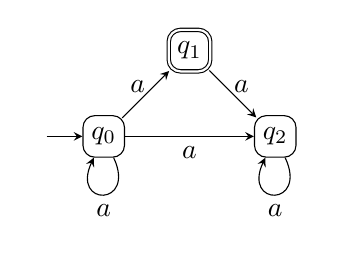
\begin{tikzpicture}[automaton]
\node[state,initial]   (0)                    {\q0};
\node[state,accepting] (1) [above right=of 0] {\q1};
\node[state]           (2) [below right=of 1] {\q2};
\path[->] (0) edge[my below,loop] node[below]           {$a$} ()
              edge[longer1]       node[pos=0.3,above](m){$a$} (1)
              edge                node[below]           {$a$} (2)
          (1) edge[longer1]       node[pos=0.7,above]   {$a$} (2)
          (2) edge[my below,loop] node[below]           {$a$} (); 
\end{tikzpicture}
}

%==============================================================================%
% Michel automata 1 to 4
%==============================================================================%
\newcommand{\labsize}{\scriptsize}  % Size of the edge labels
\newcommand{\MichelOne}{
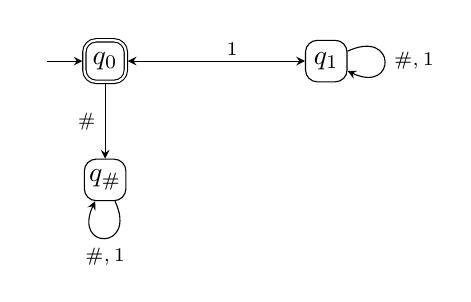
\begin{tikzpicture}[automaton]
% Starting node and # node
\node[state,initial,accepting] (0)               {\q0};
\node[state,yshift=-0.2cm]                   (x) [below=of 0]  {\q\#};
\draw[->] (0) edge node[left] {\labsize\#} (x);
\draw[->] (x) edge[my below,loop] node[below] {\labsize $\#,1$} ();
% Node 1
\node[state,xshift=1.5cm]        (1) [right=of 0]  {\q1};
\draw[<->] (0) edge node[above,xshift=2mm,yshift=-0.5mm] {\labsize $1$} (1);
\draw[->] (1) edge[my right,loop] node[right] {\labsize $\#,1$} ();
\end{tikzpicture}
}

\newcommand{\MichelTwo}{
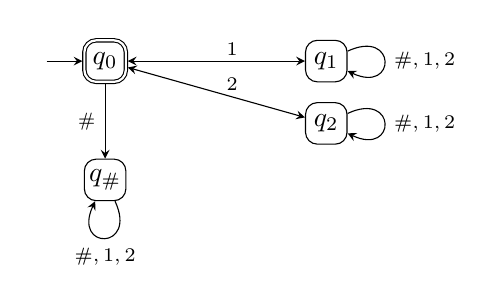
\begin{tikzpicture}[automaton]
% Starting node and # node
\node[state,initial,accepting] (0)               {\q0};
\node[state,yshift=-0.2cm]                   (x) [below=of 0]  {\q\#};
\draw[->] (0) edge node[left] {\labsize\#} (x);
\draw[->] (x) edge[my below,loop] node[below] {\labsize $\#,1,2$} ();
% Node 1
\node[state,xshift=1.5cm]        (1) [right=of 0]  {\q1};
\draw[<->] (0) edge node[above,xshift=2mm,yshift=-0.5mm] {\labsize $1$} (1);
\draw[->] (1) edge[my right,loop] node[right] {\labsize $\#,1,2$} ();
% Node 2
\node[state,yshift=0.5cm]      (2) [below=of 1]  {\q2};
\draw[<->] (0) edge node[above,xshift=2mm,yshift=-1mm] {\labsize $2$} (2);
\draw[->] (2) edge[my right,loop] node[right] {\labsize $\#,1,2$} ();
\end{tikzpicture}
}

\newcommand{\MichelThree}{
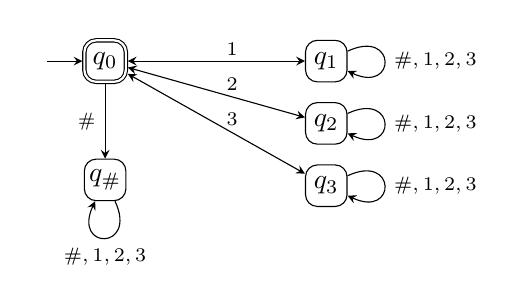
\begin{tikzpicture}[automaton]
% Starting node and # node
\node[state,initial,accepting] (0)               {\q0};
\node[state,yshift=-0.2cm]                   (x) [below=of 0]  {\q\#};
\draw[->] (0) edge node[left] {\labsize\#} (x);
\draw[->] (x) edge[my below,loop] node[below] {\labsize $\#,1,2,3$} ();
% Node 1
\node[state,xshift=1.5cm]        (1) [right=of 0]  {\q1};
\draw[<->] (0) edge node[above,xshift=2mm,yshift=-0.5mm] {\labsize $1$} (1);
\draw[->] (1) edge[my right,loop] node[right] {\labsize $\#,1,2,3$} ();
% Node 2
\node[state,yshift=0.5cm]      (2) [below=of 1]  {\q2};
\draw[<->] (0) edge node[above,xshift=2mm,yshift=-1mm] {\labsize $2$} (2);
\draw[->] (2) edge[my right,loop] node[right] {\labsize $\#,1,2,3$} ();
% Node 3
\node[state,yshift=0.5cm]      (3) [below=of 2]  {\q3};
\draw[<->] (0) edge node[above,xshift=2mm,yshift=-1.5mm] {\labsize $3$} (3);
\draw[->] (3) edge[my right,loop] node[right] {\labsize $\#,1,2,3$} ();
\end{tikzpicture}
}

\newcommand{\MichelFour}{
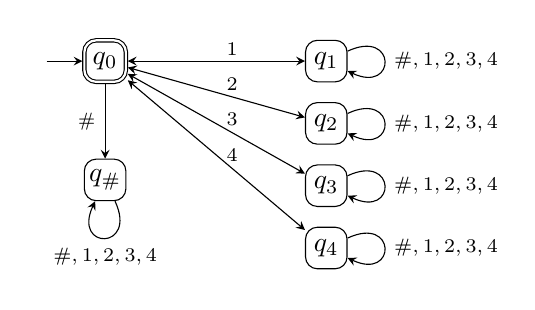
\begin{tikzpicture}[automaton]
% Starting node and # node
\node[state,initial,accepting] (0)               {\q0};
\node[state,yshift=-0.2cm]                   (x) [below=of 0]  {\q\#};
\draw[->] (0) edge node[left] {\labsize\#} (x);
\draw[->] (x) edge[my below,loop] node[below] {\labsize $\#,1,2,3,4$} ();
% Node 1
\node[state,xshift=1.5cm]        (1) [right=of 0]  {\q1};
\draw[<->] (0) edge node[above,xshift=2mm,yshift=-0.5mm] {\labsize $1$} (1);
\draw[->] (1) edge[my right,loop] node[right] {\labsize $\#,1,2,3,4$} ();
% Node 2
\node[state,yshift=0.5cm]      (2) [below=of 1]  {\q2};
\draw[<->] (0) edge node[above,xshift=2mm,yshift=-1mm] {\labsize $2$} (2);
\draw[->] (2) edge[my right,loop] node[right] {\labsize $\#,1,2,3,4$} ();
% Node 3
\node[state,yshift=0.5cm]      (3) [below=of 2]  {\q3};
\draw[<->] (0) edge node[above,xshift=2mm,yshift=-1.5mm] {\labsize $3$} (3);
\draw[->] (3) edge[my right,loop] node[right] {\labsize $\#,1,2,3,4$} ();
% Node 4
\node[state,yshift=0.5cm]      (4) [below=of 3]  {\q4};
\draw[<->] (0) edge node[above,xshift=2mm,yshift=-2mm] {\labsize $4$} (4);
\draw[->] (4) edge[my right,loop] node[right] {\labsize $\#,1,2,3,4$} ();
\end{tikzpicture}
}

%==============================================================================%
% Level symbols for trees and run DAG
%==============================================================================%
\newcommand{\LevelSymbols}{
\begin{tikzpicture}[tree,every tree node/.style={draw=none},edge from parent/.style={draw=none},l/.style={pos=0.3}]
\Tree [ \edge node[l]{$a$}; [ \edge node[l]{$a$}; [ \edge node[l]{$a$}; [ \edge node[l]{$a$}; {} ] ] ] ]
\end{tikzpicture}
}

%==============================================================================%
% Run tree
%==============================================================================%
\newcommand{\RunTree}{
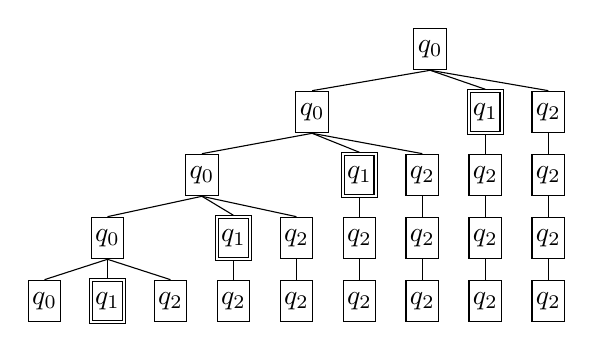
\begin{tikzpicture}[tree]
\Tree
[.\node{\q0}; [.\node{\q0}; [.\node(m){\q0}; [.\node{\q0};    \node{\q0};
                                                              \node[a]{\q1};
                                                              \node{\q2}; ]
                                             [.\node[a]{\q1}; \node{\q2}; ]
                                             [.\node{\q2};    \node{\q2}; ] ]
                            [.\node[a]{\q1}; [.\node{\q2};    \node{\q2}; ] ]
                            [.\node{\q2};    [.\node{\q2};    \node{\q2}; ] ] ]
              [.\node[a]{\q1}; [.\node{\q2}; [.\node{\q2};    \node{\q2}; ] ] ]
              [.\node{\q2}; [.\node{\q2};    [.\node{\q2};    \node{\q2}; ] ] ]]
%\node[anchor=base,xshift=-4cm] at (m.base) {$\mathcal{T}^A_{a^\omega}=$};
\end{tikzpicture}
\LevelSymbols
}

%==============================================================================%
% Subset-construction tree
%==============================================================================%
\newcommand{\SubsetConstructionTree}{
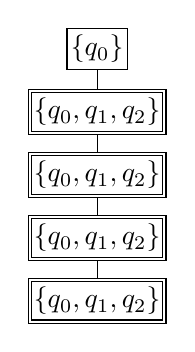
\begin{tikzpicture}[tree]
\Tree
[.\node{\qq0}; [.\node[a]{\qqqq012}; [.\node[a]{\qqqq012}; [.\node[a]{\qqqq012}; \node[a]{\qqqq012}; ] ] ] ]
\end{tikzpicture}
\LevelSymbols
}

%==============================================================================%
% Split tree (left-to-right)
%==============================================================================%
\newcommand{\SplitTreeLeftRight}{
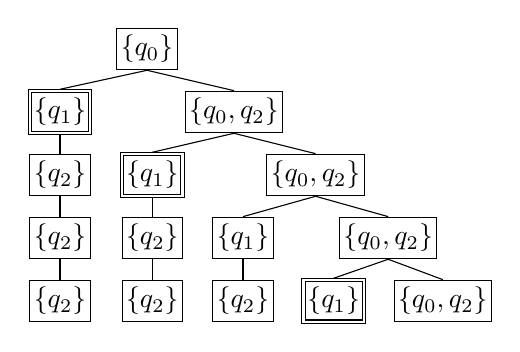
\begin{tikzpicture}[tree]
\Tree
[.\node{\qq0}; [.\node[a]{\qq1};  [.\node(m){\qq2};  [.\node{\qq2};  \node{\qq2}; ] ] ]
              [.\node{\qqq02}; [.\node[a]{\qq1};  [.\node{\qq2};  \node{\qq2}; ] ]
                             [.\node{\qqq02}; [.\node{\qq1};  \node{\qq2}; ]
                                            [.\node{\qqq02}; \node[a]{\qq1};
                                                           \node{\qqq02}; ] ] ] ]
%\node[anchor=base,xshift=-1.5cm] at (m.base) {$\mathcal{S}^A_{a^\omega}=$};
\end{tikzpicture}
\LevelSymbols
}

%==============================================================================%
% Split tree (right-to-left)
%==============================================================================%
\newcommand{\SplitTreeRightLeft}{
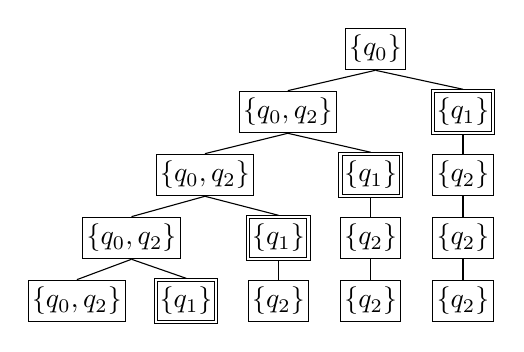
\begin{tikzpicture}[tree]
\Tree
[.\node{\qq0}; [.\node{\qqq02};  [.\node{\qqq02};  [.\node{\qqq02};  \node{\qqq02};
                                                                     \node[a]{\qq1}; ]
                                                   [.\node[a]{\qq1}; \node{\qq2}; ] ]
                                 [.\node[a]{\qq1}; [.\node{\qq2};    \node{\qq2}; ] ] ]
               [.\node[a]{\qq1}; [.\node{\qq2};    [.\node{\qq2};    \node{\qq2}; ] ] ] ]
\end{tikzpicture}
\LevelSymbols
}

%==============================================================================%
% Reduced split tree left-to-right
%==============================================================================%
\newcommand{\ReducedSplitTreeLeftRight}{
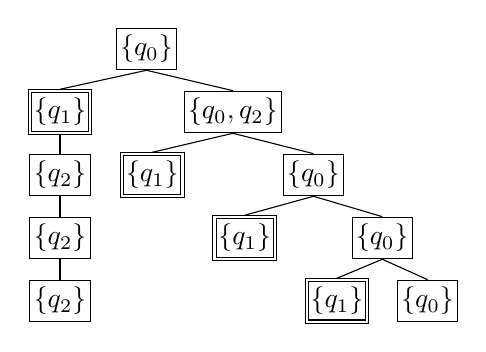
\begin{tikzpicture}[tree]
\Tree
[.\node{\qq0}; [.\node[a]{\qq1}; [.\node(m){\qq2}; [.\node{\qq2}; \node{\qq2}; ] ] ]
               [.\node{\qqq02};    \node[a]{\qq1};
                                 [.\node{\qq0};      \node[a]{\qq1};
                                                   [.\node{\qq0}; \node[a]{\qq1};
                                                            \node{\qq0}; ] ] ] ]
%\node[anchor=base,xshift=-1.5cm] at (m.base) {$\mathcal{R}^A_{a^\omega}=$};
\end{tikzpicture}
\LevelSymbols
}

%==============================================================================%
% Reduced split tree right-to-left
%==============================================================================%
\newcommand{\ReducedSplitTreeRightLeft}{
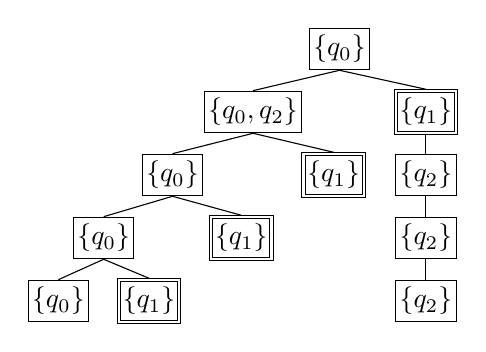
\begin{tikzpicture}[tree]
\Tree
[.\node{\qq0}; [.\node{\qqq02}; [.\node(m){\qq0}; [.\node{\qq0}; \node{\qq0};
                                                            \node[a]{\qq1}; ] 
                                                \node[a]{\qq1}; ]
                               \node[a]{\qq1}; ]
              [.\node[a]{\qq1};  [.\node{\qq2};    [.\node{\qq2}; \node{\qq2}; ] ] ] ]
%\node[anchor=base,xshift=-1.5cm] at (m.base) {$\mathcal{R}^A_{a^\omega}=$};
\end{tikzpicture}
\LevelSymbols
}

%==============================================================================%
% Pair of slices of a reduced split tree (right-to-left)
%==============================================================================%
\newcommand{\SlicesOne}{
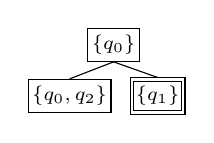
\begin{tikzpicture}[tree,level distance=\myvdistsmall,sibling distance=\myhdistsmall]
\scriptsize
\Tree
[.\node{\qq0}; [.\node   {\qqq02}; ]
               [.\node[a]{\qq1};   ] ] 
\end{tikzpicture}
}

\newcommand{\SlicesTwo}{
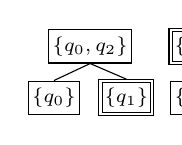
\begin{tikzpicture}[tree,level distance=\myvdistsmall,sibling distance=\myhdistsmall]
\scriptsize
\Tree
[.\node{\qqq02}; [.\node   {\qq0}; ]
                 [.\node[a]{\qq1}; ] ]
\hspace{1.35cm}
\Tree
[.\node[a]{\qq1};   \node{\qq2}; ]
\end{tikzpicture}
}

\newcommand{\SlicesThree}{
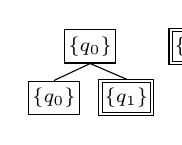
\begin{tikzpicture}[tree,level distance=\myvdistsmall,sibling distance=\myhdistsmall]
\scriptsize
\Tree
[.\node{\qq0}; [.\node   {\qq0}; ]
               [.\node[a]{\qq1}; ] ]
\hspace{1.35cm}
\Tree
[.\node[a]{\qq1}; ]
\hspace{0.9cm}
\Tree
[.\node{\qq2}; \node{\qq2}; ]
\end{tikzpicture}
}

%==============================================================================%
% Run DAG
%==============================================================================%
\newcommand{\RunDAG}{
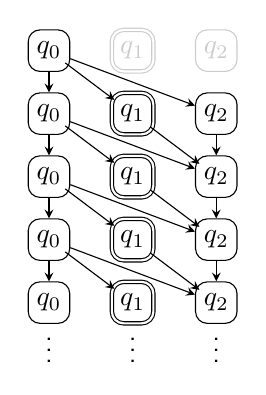
\begin{tikzpicture}[dag]  
\matrix[every node/.style={my state}]{
  \node (00) {\q0}; \& \node[a,ghost] (01) {\q1}; \& \node[ghost] (02) {\q2}; \\
  \node (10) {\q0}; \& \node[a] (11) {\q1}; \& \node (12) {\q2}; \\
  \node (20) {\q0}; \& \node[a] (21) {\q1}; \& \node (22) {\q2}; \\
  \node (30) {\q0}; \& \node[a] (31) {\q1}; \& \node (32) {\q2}; \\
  \node (40) {\q0}; \& \node[a] (41) {\q1}; \& \node (42) {\q2}; \\
  \node[inv,yshift=0.3cm] {$\vdots$}; \& \node[inv,yshift=0.3cm] {$\vdots$}; \& \node[inv,yshift=0.3cm] {$\vdots$}; \\
};
\path[->]
  (00) edge          (10) edge[longer2] (11) edge (12)
  (10) edge          (20) edge[longer2] (21) edge (22)
  (11) edge[longer2] (22)
  (12) edge          (22)
  (20) edge          (30) edge[longer2] (31) edge (32)
  (21) edge[longer2] (32)
  (22) edge          (32)
  (30) edge          (40) edge[longer2] (41) edge (42)
  (31) edge[longer2] (42)
  (32) edge          (42);  
%\node[anchor=base,xshift=-1.5cm] at (20.base) {$\mathcal{G}^A_{a^\omega}=$};      
\end{tikzpicture}
\LevelSymbols
}

%==============================================================================%
% Slices
%==============================================================================%
\newcommand{\Slices}{
%\LevelSymbols
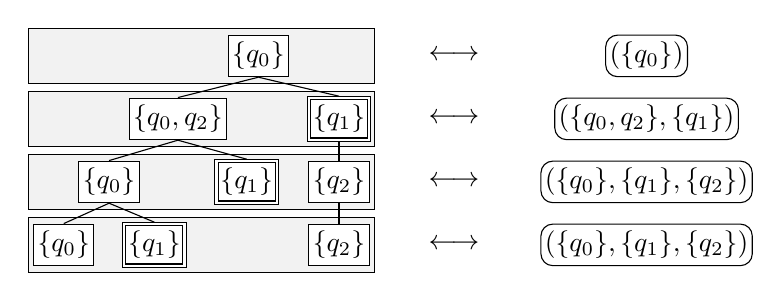
\begin{tikzpicture}[
  tree,
  every tree node/.append style={fill=white},
  automaton,
  frame/.style={
    draw,rectangle,
    minimum width=4.4cm,
    minimum height=2em,
    fill=black!5
  }
]
\Tree
% [.\node{\qq0}; [.\node{\qqq02}; [.\node(m){\qq0}; [.\node{\qq0}; \node{\qq0};
%                                                             \node[a]{\qq1}; ] 
%                                                 \node[a]{\qq1}; ]
%                                \node[a]{\qq1}; ]
%               [.\node[a]{\qq1};  [.\node(m){\qq2};    [.\node{\qq2}; \node{\qq2}; ] ] ] ]
[.\node{\qq0}; [.\node{\qqq02};  [ .\node{\qq0};     \node{\qq0};
                                                     \node[a]{\qq1}; ]
                                   \node[a]{\qq1}; ]
               [.\node[a]{\qq1}; [.\node{\qq2};      \node(m){\qq2}; ] ] ]
\begin{scope}[on background layer]
\node[frame,anchor=east,xshift=0.7mm] (level3) at (m.east) {};
\node[frame,yshift=\myvdist]          (level2) at (level3) {};
\node[frame,yshift=\myvdist]          (level1) at (level2) {};
\node[frame,yshift=\myvdist]          (level0) at (level1) {};
\end{scope}
\begin{scope}[every node/.style={xshift=1cm}]
\node (arrow0) at (level0.east) {$\longleftrightarrow$};
\node (arrow1) at (level1.east) {$\longleftrightarrow$};
\node (arrow2) at (level2.east) {$\longleftrightarrow$};
\node (arrow3) at (level3.east) {$\longleftrightarrow$};
\end{scope}
\begin{scope}[every node/.style={xshift=2cm}]
\node[state] (s0) at (arrow0.east) {$(\qm0)$};
\node[state] (s1) at (arrow1.east) {$(\qqm02,\qm1)$};
\node[state] (s2) at (arrow2.east) {$(\qm0,\qm1,\qm2)$};
\node[state] (s3) at (arrow3.east) {$(\qm0,\qm1,\qm2)$};
\end{scope}
% \path[->] (s0) edge node[right] {$a$} (s1)
%           (s1) edge node[right] {$a$} (s2)
%           (s2) edge[my below,loop] node[below] {$a$} ();
\end{tikzpicture}
}

%==============================================================================%
% Upper part
%==============================================================================%
\newcommand{\UpperPart}{
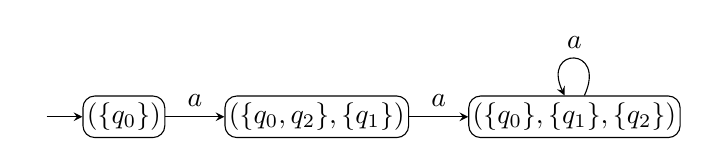
\begin{tikzpicture}[automaton]
\node[state,initial] (0)              {$(\qm0)$};
\node[state]         (1) [right=of 0] {$(\qqm02,\qm1)$};
\node[state]         (2) [right=of 1] {$(\qm0,\qm1,\qm2)$};
\path[->] (0) edge node[above]{$a$} (1)
          (1) edge node[above]{$a$} (2)
          (2) edge[my above,loop] node[above]{$a$} ();
\end{tikzpicture}
}

\newcommand{\UpperPartA}{
\begin{tikzpicture}[automaton,node distance=\myndistsmall]
\scriptsize
\node[state,initial] (0)              {$(\qm0)$};
\begin{scope}[opacity=0]
  \node[state]         (1) [right=of 0] {$(\qqm02,\qm1)$};
  \node[state]         (2) [right=of 1] {$(\qm0,\qm1,\qm2)$};
  \path[->] (0) edge node[above]{$a$} (1)
            (1) edge node[above]{$a$} (2)
            (2) edge[my above,loop] node[above]{$a$} ();
\end{scope}
\end{tikzpicture}
}

\newcommand{\UpperPartB}{
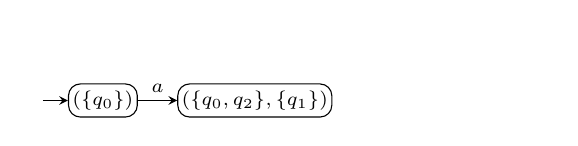
\begin{tikzpicture}[automaton,node distance=\myndistsmall]
\scriptsize
\node[state,initial] (0)              {$(\qm0)$};
\node[state]         (1) [right=of 0] {$(\qqm02,\qm1)$};
\begin{scope}[opacity=0]
  \node[state]         (2) [right=of 1] {$(\qm0,\qm1,\qm2)$};
\end{scope}
\path[->] (0) edge node[above]{$a$} (1);
\begin{scope}[opacity=0]
  \path
            (1) edge node[above]{$a$} (2)
            (2) edge[my above,loop] node[above]{$a$} ();
\end{scope}
\end{tikzpicture}
}

\newcommand{\UpperPartC}{
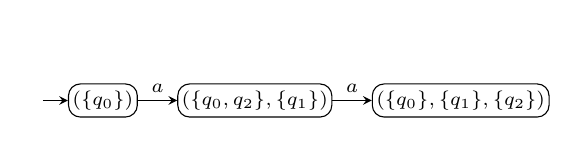
\begin{tikzpicture}[automaton,node distance=\myndistsmall]
\scriptsize
\node[state,initial] (0)              {$(\qm0)$};
\node[state]         (1) [right=of 0] {$(\qqm02,\qm1)$};
\node[state]         (2) [right=of 1] {$(\qm0,\qm1,\qm2)$};
\path[->] (0) edge node[above]{$a$} (1)
          (1) edge node[above]{$a$} (2);
\begin{scope}[opacity=0]
\path 
            (2) edge[my above,loop] node[above]{$a$} ();
\end{scope}
\end{tikzpicture}
}

\newcommand{\UpperPartD}{
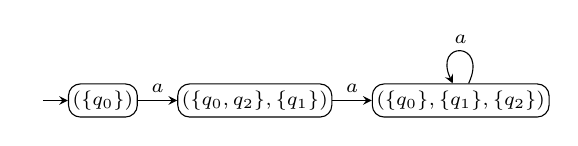
\begin{tikzpicture}[automaton,node distance=\myndistsmall]
\scriptsize
\node[state,initial] (0)              {$(\qm0)$};
\node[state]         (1) [right=of 0] {$(\qqm02,\qm1)$};
\node[state]         (2) [right=of 1] {$(\qm0,\qm1,\qm2)$};
\path[->] (0) edge node[above]{$a$} (1)
          (1) edge node[above]{$a$} (2)
          (2) edge[my above,loop] node[above]{$a$} ();
\end{tikzpicture}
}

%==============================================================================%
% Complement automaton B
%==============================================================================%
\newcommand{\Complement}{
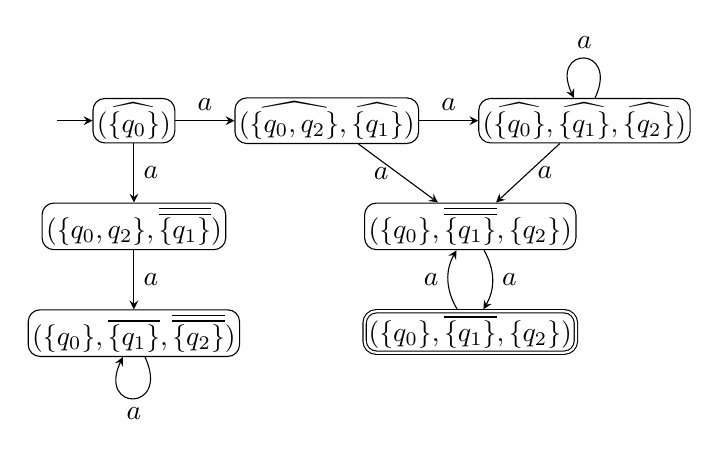
\begin{tikzpicture}[automaton]
\node[state,initial]   (0)               {$(\cl^{\qm0})$};
\node[state]           (1)  [right=of 0] {$(\cl^{\qqm02},\cl^{\qm1})$};
\node[state]           (2)  [right=of 1] {$(\cl^{\qm0},\cl^{\qm1},\cl^{\qm2})$};
\node[state]           (01) [below=of 0] {$(\qqm02,\cl2{\qm1})$};
\node[state,xshift=1cm](11) [right=of 01]{$(\qm0,\cl2{\qm1},\qm2)$};
\node[state]           (02) [below=of 01]{$(\qm0,\cl1{\qm1},\cl2{\qm2})$};
\node[state,accepting] (12) [below=of 11]{$(\qm0,\cl1{\qm1},\qm2)$};
\path[->] (0)  edge                node[above]{$a$} (1)
          (1)  edge                node[above]{$a$} (2)
          (2)  edge[my above,loop] node[above]{$a$} ()
          (0)  edge                node[right]{$a$} (01)
          (01) edge                node[right]{$a$} (02)
          (02) edge[my below,loop] node[below]{$a$} ()
          (1)  edge                node[left] {$a$} (11)
          (11) edge[bend left]     node[right]{$a$} (12)
          (12) edge[bend left]     node[left] {$a$} (11)
          (2)  edge                node[right]{$a$} (11);
\end{tikzpicture}
}

% Complement of the example automaton by applying the M2 optimisation
\newcommand{\ComplementWithMTwo}{
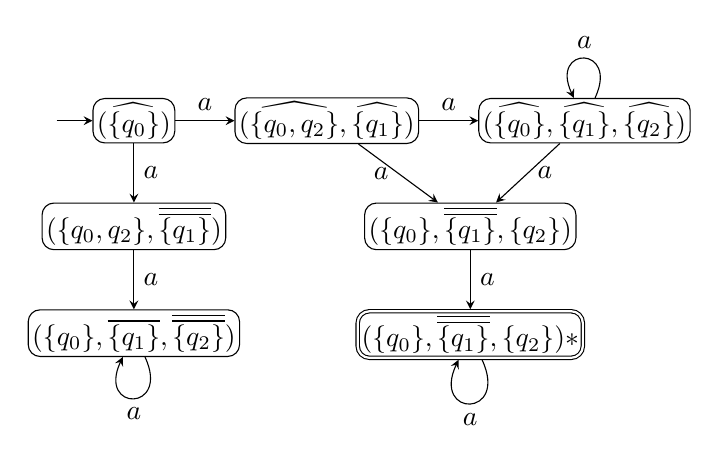
\begin{tikzpicture}[automaton]
\node[state,initial]   (0)               {$(\cl^{\qm0})$};
\node[state]           (1)  [right=of 0] {$(\cl^{\qqm02},\cl^{\qm1})$};
\node[state]           (2)  [right=of 1] {$(\cl^{\qm0},\cl^{\qm1},\cl^{\qm2})$};
\node[state]           (01) [below=of 0] {$(\qqm02,\cl2{\qm1})$};
\node[state,xshift=1cm](11) [right=of 01]{$(\qm0,\cl2{\qm1},\qm2)$};
\node[state]           (02) [below=of 01]{$(\qm0,\cl1{\qm1},\cl2{\qm2})$};
\node[state,accepting] (12) [below=of 11]{$(\qm0,\cl2{\qm1},\qm2)*$};
\path[->] (0)  edge                node[above]{$a$} (1)
          (1)  edge                node[above]{$a$} (2)
          (2)  edge[my above,loop] node[above]{$a$} ()
          (0)  edge                node[right]{$a$} (01)
          (01) edge                node[right]{$a$} (02)
          (02) edge[my below,loop] node[below]{$a$} ()
          (1)  edge                node[left] {$a$} (11)
          (11) edge                node[right]{$a$} (12)
          (12) edge[my below,loop] node[below]{$a$} ()
          (2)  edge                node[right]{$a$} (11);
\end{tikzpicture}
}

\newcommand{\ComplementA}{
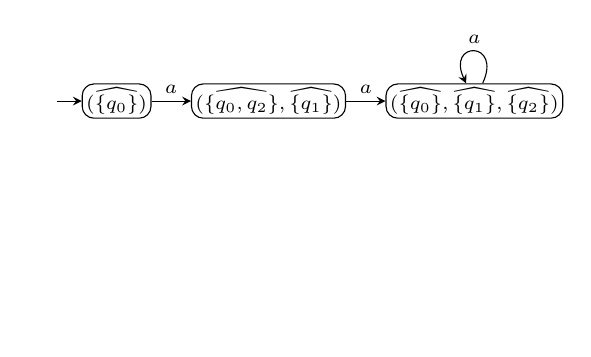
\begin{tikzpicture}[automaton,node distance=\myndistsmall]
\scriptsize
\node[state,initial]   (0)               {$(\cl^{\qm0})$};
\node[state]           (1)  [right=of 0] {$(\cl^{\qqm02},\cl^{\qm1})$};
\node[state]           (2)  [right=of 1] {$(\cl^{\qm0},\cl^{\qm1},\cl^{\qm2})$};
\begin{scope}[opacity=0]
  \node[state]           (01) [below=of 0] {$(\qqm02,\cl2{\qm1})$};
  \node[state,xshift=1cm](11) [right=of 01]{$(\qm0,\cl2{\qm1},\qm2)$};
  \node[state]           (02) [below=of 01]{$(\qm0,\cl1{\qm1},\cl2{\qm2})$};
  \node[state,accepting] (12) [below=of 11]{$(\qm0,\cl1{\qm1},\qm2)$};
\end{scope}
\path[->] (0)  edge                node[above]{$a$} (1)
          (1)  edge                node[above]{$a$} (2)
          (2)  edge[my above,loop] node[above]{$a$} ();
\begin{scope}[opacity=0]
  \path
            (0)  edge                node[right]{$a$} (01)
            (01) edge                node[right]{$a$} (02)
            (02) edge[my below,loop] node[below]{$a$} ()
            (1)  edge                node[left] {$a$} (11)
            (11) edge[bend left]     node[right]{$a$} (12)
            (12) edge[bend left]     node[left] {$a$} (11)
            (2)  edge                node[right]{$a$} (11);
\end{scope}
\end{tikzpicture}
}

\newcommand{\ComplementB}{
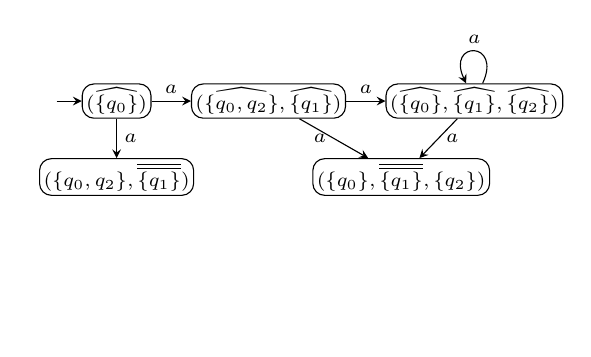
\begin{tikzpicture}[automaton,node distance=\myndistsmall]
\scriptsize
\node[state,initial]   (0)               {$(\cl^{\qm0})$};
\node[state]           (1)  [right=of 0] {$(\cl^{\qqm02},\cl^{\qm1})$};
\node[state]           (2)  [right=of 1] {$(\cl^{\qm0},\cl^{\qm1},\cl^{\qm2})$};
\node[state]           (01) [below=of 0] {$(\qqm02,\cl2{\qm1})$};
\node[state,xshift=1cm](11) [right=of 01]{$(\qm0,\cl2{\qm1},\qm2)$};
\begin{scope}[opacity=0]
  \node[state]           (02) [below=of 01]{$(\qm0,\cl1{\qm1},\cl2{\qm2})$};
  \node[state,accepting,opacity=0] (12) [below=of 11]{$(\qm0,\cl1{\qm1},\qm2)$};
\end{scope}
\path[->] (0)  edge                node[above]{$a$} (1)
          (1)  edge                node[above]{$a$} (2)
          (2)  edge[my above,loop] node[above]{$a$} ()
          (0)  edge                node[right]{$a$} (01)
          (1)  edge                node[left] {$a$} (11)
          (2)  edge                node[right]{$a$} (11);
\begin{scope}[opacity=0]
  \path
            (01) edge                node[right]{$a$} (02)
            (02) edge[my below,loop] node[below]{$a$} ()
            (11) edge[bend left]     node[right]{$a$} (12)
            (12) edge[bend left]     node[left] {$a$} (11);
\end{scope}
\end{tikzpicture}
}

\newcommand{\ComplementC}{
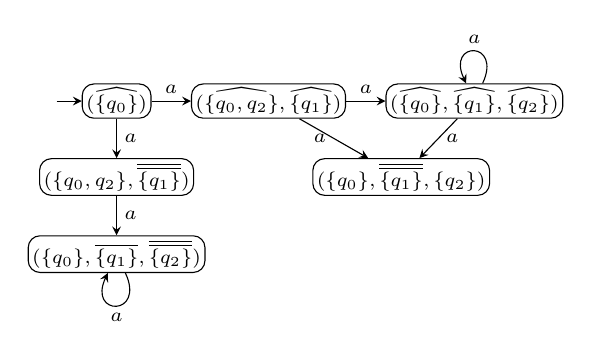
\begin{tikzpicture}[automaton,node distance=\myndistsmall]
\scriptsize
\node[state,initial]   (0)               {$(\cl^{\qm0})$};
\node[state]           (1)  [right=of 0] {$(\cl^{\qqm02},\cl^{\qm1})$};
\node[state]           (2)  [right=of 1] {$(\cl^{\qm0},\cl^{\qm1},\cl^{\qm2})$};
\node[state]           (01) [below=of 0] {$(\qqm02,\cl2{\qm1})$};
\node[state,xshift=1cm](11) [right=of 01]{$(\qm0,\cl2{\qm1},\qm2)$};
\node[state]           (02) [below=of 01]{$(\qm0,\cl1{\qm1},\cl2{\qm2})$};
\begin{scope}[opacity=0]
  \node[state,accepting,opacity=0] (12) [below=of 11]{$(\qm0,\cl1{\qm1},\qm2)$};
\end{scope}
\path[->] (0)  edge                node[above]{$a$} (1)
          (1)  edge                node[above]{$a$} (2)
          (2)  edge[my above,loop] node[above]{$a$} ()
          (0)  edge                node[right]{$a$} (01)
          (1)  edge                node[left] {$a$} (11)
          (2)  edge                node[right]{$a$} (11)
          (01) edge                node[right]{$a$} (02)
          (02) edge[my below,loop] node[below]{$a$} ();
\begin{scope}[opacity=0]
  \path
            (11) edge[bend left]     node[right]{$a$} (12)
            (12) edge[bend left]     node[left] {$a$} (11);
\end{scope}
\end{tikzpicture}
}

\newcommand{\ComplementD}{
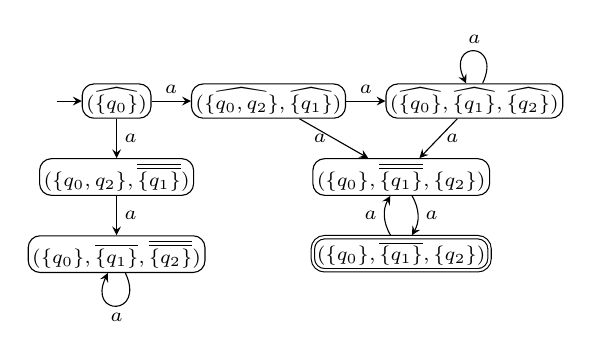
\begin{tikzpicture}[automaton,node distance=\myndistsmall]
\scriptsize
\node[state,initial]   (0)               {$(\cl^{\qm0})$};
\node[state]           (1)  [right=of 0] {$(\cl^{\qqm02},\cl^{\qm1})$};
\node[state]           (2)  [right=of 1] {$(\cl^{\qm0},\cl^{\qm1},\cl^{\qm2})$};
\node[state]           (01) [below=of 0] {$(\qqm02,\cl2{\qm1})$};
\node[state,xshift=1cm](11) [right=of 01]{$(\qm0,\cl2{\qm1},\qm2)$};
\node[state]           (02) [below=of 01]{$(\qm0,\cl1{\qm1},\cl2{\qm2})$};
\node[state,accepting] (12) [below=of 11]{$(\qm0,\cl1{\qm1},\qm2)$};
\path[->] (0)  edge                node[above]{$a$} (1)
          (1)  edge                node[above]{$a$} (2)
          (2)  edge[my above,loop] node[above]{$a$} ()
          (0)  edge                node[right]{$a$} (01)
          (01) edge                node[right]{$a$} (02)
          (02) edge[my below,loop] node[below]{$a$} ()
          (1)  edge                node[left] {$a$} (11)
          (11) edge[bend left]     node[right]{$a$} (12)
          (12) edge[bend left]     node[left] {$a$} (11)
          (2)  edge                node[right]{$a$} (11);
\end{tikzpicture}
}

%==============================================================================%
% Component relations between two states
%==============================================================================%
\newcommand{\PredCompsOne}{
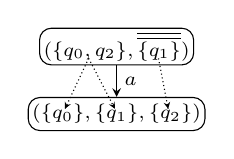
\begin{tikzpicture}[automaton,node distance=0.4cm]
\scriptsize
\node[state] (1)              {$(\qqm02,\cl2{\qm1})$};
\node[state] (2) [below=of 1] {$(\qm0, \qm1, \qm2)$};
\draw[densely dotted,small arrow]
($(1.south east)!0.23!(1.south west)+(0,0.9mm)$)
    -- ($(2.north east)!0.21!(2.north west)-(0,1.5mm)$);
\draw[densely dotted,small arrow]
($(1.south east)!0.68!(1.south west)+(0,0.9mm)$)
    -- ($(2.north east)!0.51!(2.north west)-(0,1.5mm)$);
\draw[densely dotted,small arrow]
($(1.south east)!0.68!(1.south west)+(0,0.9mm)$)
    -- ($(2.north east)!0.79!(2.north west)-(0,1.5mm)$);
\path[->] (1) edge node[right] {$a$} (2);
\end{tikzpicture}
}

\newcommand{\PredCompsTwo}{
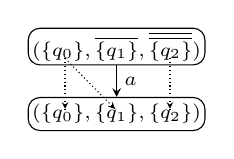
\begin{tikzpicture}[automaton,node distance=0.4cm]
\scriptsize
\node[state] (1)              {$(\qm0,\cl1{\qm1},\cl2{\qm2})$};
\node[state] (2) [below=of 1] {$(\qm0, \qm1, \qm2)$};
\draw[densely dotted,small arrow]
($(1.south east)!0.2!(1.south west)+(0,0.9mm)$)
    -- ($(2.north east)!0.2!(2.north west)-(0,1.5mm)$);
\draw[densely dotted,small arrow]
($(1.south east)!0.79!(1.south west)+(0,0.9mm)$)
    -- ($(2.north east)!0.51!(2.north west)-(0,1.5mm)$);
\draw[densely dotted,small arrow]
($(1.south east)!0.79!(1.south west)+(0,0.9mm)$)
    -- ($(2.north east)!0.79!(2.north west)-(0,1.5mm)$);
\path[->] (1) edge node[right] {$a$} (2);
\end{tikzpicture}
}

\newcommand{\PredCompsThree}{
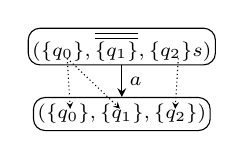
\begin{tikzpicture}[automaton,node distance=0.4cm]
\scriptsize
\node[state] (1)              {$(\qm0,\cl2{\qm1}, \qm2s)$};
\node[state] (2) [below=of 1] {$(\qm0, \qm1, \qm2)$};
\draw[densely dotted,small arrow]
($(1.south east)!0.2!(1.south west)+(0,0.9mm)$)
    -- ($(2.north east)!0.2!(2.north west)-(0,1.5mm)$);
\draw[densely dotted,small arrow]
($(1.south east)!0.79!(1.south west)+(0,0.9mm)$)
    -- ($(2.north east)!0.51!(2.north west)-(0,1.5mm)$);
\draw[densely dotted,small arrow]
($(1.south east)!0.79!(1.south west)+(0,0.9mm)$)
    -- ($(2.north east)!0.79!(2.north west)-(0,1.5mm)$);
\path[->] (1) edge node[right] {$a$} (2);
\end{tikzpicture}
}

%==============================================================================%
% Run types
%==============================================================================%
\newcommand{\RunTypes}{
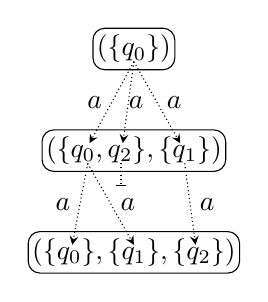
\begin{tikzpicture}[automaton]
\node[state] (0)              {$(\qm0)$};
\node[state] (1) [below=of 0] {$(\qqm02,\qm1)$};
\node[state] (2) [below=of 1] {$(\qm0,\qm1,\qm2)$};
\path[->,densely dotted]
($(0.south)+(0,1.1mm)$)
    edge node[right]     {$a$} ($(1.north east)!0.25!(1.north west)-(0,1.75mm)$)
    edge node[xshift=1mm]{$a$} ($(1.north east)!0.56!(1.north west)-(0,1.75mm)$)
    edge node[left]      {$a$} ($(1.north east)!0.74!(1.north west)-(0,1.75mm)$)
($(1.south east)!0.225!(1.south west)+(0,1.1mm)$)
    edge node[right]{$a$} ($(2.north east)!0.21!(2.north west)-(0,1.75mm)$)
($(1.south east)!0.75!(1.south west)+(0,1.1mm)$)
    edge node[right]{$a$} ($(2.north east)!0.50!(2.north west)-(0,1.75mm)$)
    edge node[left] {$a$} ($(2.north east)!0.79!(2.north west)-(0,1.75mm)$);
\draw[-{Bar[width=1.25mm]},densely dotted]
    ($(1.south east)!0.57!(1.south west)+(0,1.1mm)$) --
    ($(1.south east)!0.57!(1.south west)-(0,1.8mm)$);
\end{tikzpicture}
\hfil
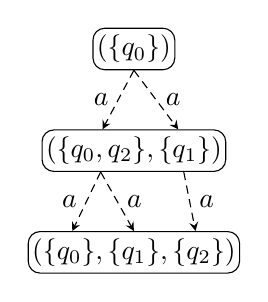
\begin{tikzpicture}[automaton]
\node[state] (0)              {$(\qm0)$};
\node[state] (1) [below=of 0] {$(\qqm02,\qm1)$};
\node[state] (2) [below=of 1] {$(\qm0,\qm1,\qm2)$};
\path[->,densely dashed]
(0.south)
    edge node[right]{$a$} ($(1.north east)!0.26!(1.north west)$)
    edge node[left] {$a$} ($(1.north east)!0.67!(1.north west)$)
($(1.south east)!0.23!(1.south west)$)
    edge node[right]{$a$} ($(2.north east)!0.21!(2.north west)$)
($(1.south east)!0.68!(1.south west)$)
    edge node[right]{$a$} ($(2.north east)!0.50!(2.north west)$)
    edge node[left] {$a$} ($(2.north east)!0.79!(2.north west)$);
\end{tikzpicture}
\hfil
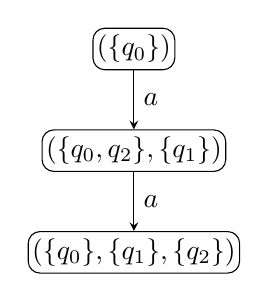
\begin{tikzpicture}[automaton]
\node[state] (0)              {$(\qm0)$};
\node[state] (1) [below=of 0] {$(\qqm02,\qm1)$};
\node[state] (2) [below=of 1] {$(\qm0,\qm1,\qm2)$};
\path[->] (0) edge node[right]{$a$} (1)
          (1) edge node[right]{$a$} (2);
\end{tikzpicture}
}

%==============================================================================%
% Expressive equivalences
%==============================================================================%
\newcommand{\Equivalences}{
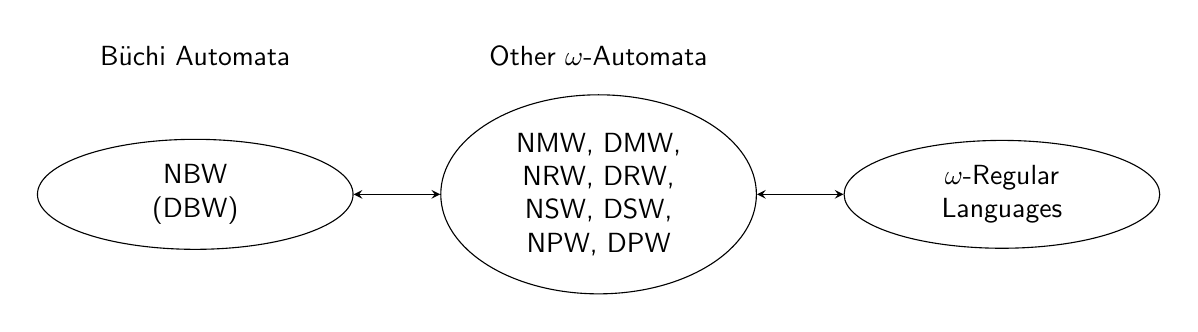
\begin{tikzpicture}[mtrx,s/.style={ellipse,draw,text width=2.6cm,align=center}]
\matrix[column sep=1.1cm,row sep=0.25cm]{
  \node               {Büchi Automata}; \& 
  \node               {Other \om-Automata}; \&
  \\
  \node[s] (left)   {NBW\\(DBW)}; \& 
  \node[s] (middle) {NMW, DMW,\\NRW, DRW,\\NSW, DSW,\\NPW, DPW}; \& 
  \node[s] (right)  {\om-Regular\\Languages}; \\
};
\path[<->] (left)   edge (middle)
           (middle) edge (right);
\end{tikzpicture}
}

%==============================================================================%
% Complementation construction
%==============================================================================%
\newcommand{\Complementation}{
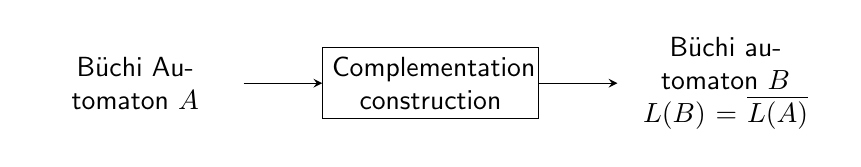
\begin{tikzpicture}[box/.style={text width=2.5cm,align=center}]
\node[box]      (l)              {Büchi Automaton $A$};
\node[draw,box] (m) [right=of l] {Complementation construction};
\node[box]      (r) [right=of m] {Büchi automaton $B$\\$L(B) = \cl1{L(A)}$}; 
\path[->] (l) edge (m)
          (m) edge (r);
\end{tikzpicture}
}


% Command for resetting table spacings
\newcommand{\tablestyle}{
  \renewcommand{\arraystretch}{1.15}
  \renewcommand{\tabcolsep}{0.2cm}
}
\tablestyle

% Shorthand commands
\newcommand{\goal}{GOAL}
\newcommand{\om}{{$\omega$}}
\newcommand{\aom}{{$a^\omega$}}
\newcommand{\ob}[1]{$\overline{\text{#1}}$}

% Custom table column: fixed width, horizontally and vertically centered
\newcolumntype{C}[1]{>{\centering\let\newline\\\arraybackslash\hspace{0pt}}m{#1}}

%==============================================================================%
% Main body
%==============================================================================%

\begin{document}
\begin{titlepage}
    \begin{center}
        \vspace*{1.2cm}
        
        \huge
        Empirical Performance Investigation of a Büchi\\Complementation Construction
        
        \vspace{2.5cm}
        
        \LARGE
        Daniel Weibel
    
        \Large
        August 2015

        \vfill

        Master's Thesis

        \vfill

        Supervised by: \\
        Prof. Dr. Ulrich Ultes-Nitsche
        
        \vspace{1.5cm}  

        \begin{tabular}{cc}
        \includegraphics[width=0.1\textwidth]{figures/unifr_logo.pdf} &
        \raisebox{0cm}{\includegraphics[width=0.4\textwidth]{figures/unifr_text.pdf}} \\
        \end{tabular}

        \vspace{0.7cm}

        \hrule
        
        \normalsize
        Foundations of Dependable Systems Group\\
        Department of Informatics\\
        University of Fribourg\\
        Switzerland
        
    \end{center}
\end{titlepage}

% Order of the front matter is: abstract, dedication, acknowledgements,
% table of contents

\begin{abstract}
Büchi automata are finite state automata on infinite words, so-called \om-automata, that have applications in domains that use an automata-theoretic approach to logic. One such domain is the automata-theoretic approach to model checking. In this approach, both, the system to be verified and the property to verify, are represented as a Büchi automaton. The verification step requires the complementation of the property automaton. However, the complementation of Büchi automata is very complex, which impedes the practical application of this approach. For this reason there is an active quest in research for finding more efficient Büchi complementation constructions, and for gaining a better understanding of Büchi complementation in general. The aim of this thesis is to contribute to a better understanding of the behaviour of Büchi complementation constructions. To this end, we empirically investigate the performance of a specific Büchi complementation construction. This includes the systematic experimentation with different variants of this construction, as well as putting this constructions into relation with other constructions. Our results highlight strengths and weaknesses of different complementation constructions, and show that there are characteristics that make the complementation of an automaton harder or easier. 
\end{abstract}

\renewcommand{\abstractname}{Acknowledgements}
\begin{abstract}
First of all, I would like to thank my supervisors Prof. Dr. Ulrich Ultes-Nitsche and Joel Allred for their support and patience during the entire time I was working on this thesis. A very special thanks goes to Dr. Ming-Hsien Tsai from the National Taiwan University. He is one of the main authors of the \goal{} tool, and steadily provided me with all the information I needed to fully integrate the plugin, developed as part of this thesis, in \goal. Without his help, the plugin would not have been possible in its present form. I am especially thankful to Assoc. Prof. Katarzyna Wac from the University of Geneva for granting me a lot of freedom in my employment at her research group. Without this flexibility, it would have been very difficult to complete the thesis within the deadlines of the university. I also would like to thank Christian Göttel for sharing information about his own thesis about a very similar topic, from which I adopted several ideas. Last but not least, I would like to thank Michael Rolli and Nico Färber from the Grid Admin Team of the University of Bern for their help regarding technical questions about the computer cluster on which the experiments of this thesis have been executed.
\end{abstract}

\dominitoc
\tableofcontents

\chapter{Introduction}
\label{chap_intro}
\minitoc
\newpage
\lettrine{A}{t the beginning} of the 1960s, a Swiss logician named Julius Richard Büchi was searching a procedure for deciding the satisfiability of formulas of the monadic second order logic with one successor (S1S). In his quest, Büchi observed that an S1S formula can be represented by a certain type of finite state automaton running on infinite words, such that this automaton accepts a word representing an interpretation of the formula, if and only if the interpretation satisfies the formula. The proof of this equivalence between S1S formulas and this type of automata is known as \textit{Büchi's Theorem}. It led Büchi to his desired decision procedure: to test whether an S1S formula $\varphi$ is satisfiable, translate it to an equivalent automaton $A$, and test whether $A$ is empty (that is, accepts no words at all). If $A$ is empty, then $\varphi$ is unsatisfiable, if $A$ is non-empty, then $\varphi$ is satisfiable.~\cite{buchi1960decision}

This thesis is about the type of automata that Büchi invented in order to solve the satisfiability problem of S1S. These automata are called \textit{Büchi automata}. Büchi automata have important applications in logic-related domains. One of them is the automata-theoretic approach to model checking, a branch of formal verification. A property to verify is specified as a Büchi automaton. The test whether the system satisfies the property requires the \textit{complementation} of this Büchi automaton. Complementing a Büchi automaton $A$ means to construct another Büchi automaton $B$ that accepts a word if and only if it is not accepted by $A$. An algorithm that takes as input a Büchi automaton and outputs the complement of this automaton is called a \textit{Büchi complementation construction}.

Büchi complementation has a very high \textit{state complexity}. This means that, given a Büchi automaton, the complement produced by a complementation construction may be extremely large. This complexity inhibits the practical application of Büchi complementation, for example in automata-theoretic model checking~\cite{2007_vardi_model_checking, 2007_vardi}. For this reason, Büchi complementation is an active research topic since the introduction of Büchi automata more than 50 years ago.

The subject of this thesis is the investigation of the performance of a specific Büchi complementation construction, the \textit{Fribourg construction}. For this investigation, we take on an empirical approach. This means that we test the construction on a set of example automata in order to evaluate the output of the construction. Generally, the smaller the complement automata that a construction generates, the better the performance of this construction. Our aim is to contribute with our results to a better understanding of the problem of Büchi complementation.

% Büchi complementation constructions are an active research topic since the introduction of Büchi automata more than 50 years ago. The reason for this persistence is that these constructions exhibit a very high \textit{state complexity}. This means that, given a Büchi automaton, the complement produced by a complementation construction may be extremely large. This complexity inhibits the practical application of Büchi complementation~\cite{2007_vardi_model_checking, 2007_vardi}. For this reason, there is an ongoing quest to find more efficient Büchi complementation constructions, and to generally better understand the problem of Büchi complementation.

This introductory chapter is structured as follows. In Section~\ref{1_context}, we present the context in which the subject of this thesis is situated. It includes Büchi automata and the problem of Büchi complementation in general, and the applications and significance of Büchi complementation. In Section~\ref{1_motivation}, we motivate the empirical approach for increasing our understanding of Büchi complementation. In Section~\ref{1_aim_scope}, we clarify the aim and scope of the thesis. Finally, in Section~\ref{1_overview}, we present the structure of the rest of this document.


% The type of automaton that Büchi used for solving this logical problem is called \textit{Büchi automaton}. The application of Büchi automata to logic, that was established by Büchi, had a large impact on other fields, especially model checking, which is a technique of formal verification. In particular, Büchi automata allow to solve the model checking question automata-theoretically, which has many advantages~\cite{1996_vardi}.

% However, there is one operation on Büchi automata that is giving a ``headache'' to the research community since the introduction of Büchi automata more than 50 years ago, namely the problem of \textit{complementation}. Algorithms for carrying out this operation, although possible\footnote{Büchi himself has proved that Büchi automata are closed under complementation~\cite{buchi1960decision}.}, turn out to be very complex, in many cases too complex for practical application. Yet, Büchi complementation has a practical application in the automata-theoretic approach to model checking. This discrepancy led to an ongoing quest for finding more efficient \textit{Büchi complementation constructions}, and generally better understanding the complexity of Büchi complementation. The work in this thesis is situated in this area of research.


% - automata-theoretic approach to logic
% - Büchi's Theorem
%   - Proof includes proving that Büchi automata are closed under complementation (most difficult part).


% At the beginning of the 1960s, a Swiss logician named Julius Richard Büchi at Michigan University was looking for a way to prove the decidability of the satisfiability of monadic second order logic with one successor (S1S). Büchi applied a trick that truly founded a new paradigm in the application of logic to theoretical computer science. He thought of interpretations of a S1S formula as infinitly long words of a formal language and designed a type of finite state automaton that accepts such a word if and only if the interpretation it represents satisfies the formula. After proving that every S1S formula can be translated to such an automaton and vice versa (Büchi's Theorem), the satisfiabilty problem of an S1S formula could be reduced to testing the non-emptiness of the corresponding automaton.

% This special type of finite state automaton was later called Büchi automaton.

\section{Context}
\label{1_context}
In this section, we describe the context of Büchi complementation. To this end, we first briefly present Büchi automata and Büchi complementation in general (Section~\ref{1_buchi_automata}). Next, we present an application of Büchi complementation in formal verification (Section~\ref{1_application}). Finally, in Section~\ref{1_importance}, we highlight the importance of Büchi complementation for this application in formal verification.

\subsection{Büchi Automata and Büchi Complementation}
\label{1_buchi_automata}
Büchi automata are finite state automata that process words of infinite length, so called \om-words. If we denote by $\Sigma$ the alphabet of a Büchi automaton, then the set of all \om-words that can be generated from this alphabet is $\Sigma^\omega$. A word $\alpha \in \Sigma^\omega$ is accepted by a Büchi automaton $A$ if it has at least one accepting run in $A$. A run is accepting if it contains an infinite number of occurrences of at least one accepting state. A run of a Büchi automaton on a word is a possibly infinite sequence of states. Deterministic Büchi automata have at most one run for each word in $\Sigma^\omega$, whereas non-deterministic Büchi automata may have multiple runs for a word.

The complement of a Büchi automaton $A$ is another Büchi automaton\footnote{Büchi automata are closed under complementation. This has been proved by Büchi~\cite{buchi1960decision}. For the sake of this proof, Büchi described the first Büchi complementation in the history of Büchi automata.} that we denote by $\cl1{A}$. Both, $A$ and $\cl1{A}$, share the same alphabet $\Sigma$. Regarding a word $\alpha \in \Sigma^\omega$, the relation between an automaton $A$ and its complement $\cl1{A}$ is as follows:

\begin{quote}
\centering
\textit{$\alpha$ is accepted by $A$ $\Longleftrightarrow$ $\alpha$ is not accepted by $\cl1{A}$}
\end{quote}

That is, all the words of $\Sigma^\omega$ that are \textit{accepted} by an automaton are \textit{rejected} by its complement, and all the words of $\Sigma^\omega$ that are \textit{rejected} by an automaton are \textit{accepted} by its complement. In other words, there is no single word of $\Sigma^\omega$ that is  accepted or rejected by \textit{both} of an automaton and its complement.

The difficulty of constructing the complement for a given Büchi automaton depends on whether this automaton is deterministic or non-deterministic. The complementation of \textit{deterministic} Büchi automata is regarded as ``easy'', because there exists a construction that can do it in polynomial time and linear space (Kurshan's construction)~\cite{Kurshan198759}. The complementation of \textit{non-deterministic} Büchi automata, however, is very complex, and therefore subject of ongoing research. Note that when in the following we talk about ``Büchi complementation'' we always refer to the complementation of \textit{non-deterministic} Büchi automata.

The main problem with the complexity of Büchi complementation is the so-called \textit{state complexity} (also known as \textit{state growth}, \textit{state blow-up} or \textit{state explosion}). This is the number of states of the output automaton in relation to the number of states of the input automaton. In particular, this means that the complement of a given Büchi automaton may be extremely large. This hinders the practical application of Büchi complementation, because the complementation operation may require very high time and computing resources. In the following we describe an important application of Büchi complementation that is negatively affected by the high state complexity of Büchi complementation.

% The complementation of Büchi automata, in particular non-deterministic Büchi automata, is commonly known as ``Büchi complementation'' or the ``Büchi complementation problem''. It is a very complex problem because it exhibits a very high state growth, which is sometimes even called state explosion (in the following, we will use the terms state growth, state explosion, and state complexity interchangeably). State growth denotes the relation of the number of states of a complement $\cl1{A}$ (output of the complementation construction) to the number of states of the automaton $A$ (input to the complementation construction). This relation is for worst-case automata exponential, even for an ideal complementation construction\footnote{Yan proved in 2007 a lower bound for the worst-case state growth of Büchi complementation of $(0.76n)^n$, where $n$ is the number of states of the initial automaton~\cite{DBLP:journals/corr/abs-0802-1226}.}. Even though the state growth that existing complementation constructions produce for many non-worst-case automata is not nearly as high as the worst case, it may still be very high. This is a serious problem, because Büchi complementation has important practical applications (as we will see next), and it is the reason that the quest for more efficient and more practical Büchi complementation constructions is still an active research topic today.


\subsection{An Application of Büchi Complementation}
\label{1_application}
In this section, we describe a specific application of Büchi complementation in formal verification. To this end, we proceed in two steps. First, we describe a general application of Büchi complementation, namely testing language containment of \om-regular languages. Next, we describe how language containment is used in a specific formal verification approach, which is called language containment approach to automata-theoretic model checking. Thus, together these two descriptions show how Büchi complementation is used in this specific model checking approach.

The following elaborations touch on various model checking concepts. For a comprehensive treatment of the interesting topic of model checking, as well as other formal verification approaches, we refer to the works by Huth~\cite{huth2004logic}, Ben-Ari~\cite{ben2012mathematical}, and Baier~\cite{baier2008principles}.

\subsubsection{Language Containment of \om-Regular Languages}
Büchi complementation is used for testing language containment of \om-regular languages. The \om-regular languages are the class of formal languages that is equivalent to non-deterministic Büchi automata\footnote{Note that deterministic Büchi automata have a lower expressivity than non-deterministic Büchi automata, and are equivalent to only a subset of the \om-regular languages.}. An \om-regular language consists of \om-words (that is, infinite words) over an alphabet $\Sigma$.

Given two \om-regular languages $L_1$ and $L_2$ over alphabet $\Sigma$ the language containment problem consists in testing whether $L_1 \subseteq L_2$. This is true if all the words of $L_1$ are also in $L_2$, and false if $L_1$ contains at least one word that is not in $L_2$. The way this problem is algorithmically solved is by testing $L_1 \cap \cl1{L_2} = \varnothing$. Here, $\cl1{L_2}$ denotes the complement language of $L_2$, which means that $\cl1{L_2}$ contains all the words of $\Sigma^\omega$ that are \textit{not} in $L_2$. The steps for testing $L_1 \cap \cl1{L_2} = \varnothing$ are the following:

\begin{enumerate}
\item Create the complement language $\cl1{L_2}$ of $L_2$
\item Create the intersection language $L_{1,\cl1{2}}$ of $L_1$ and $\cl1{L_2}$
\item Test whether $L_{1,\cl1{2}}$ is empty (that is, contains no words at all)
\end{enumerate}

Thus, the language containment problem is reduced to three operations on languages: \textit{complementation}, \textit{intersection}, and \textit{emptiness testing}. A common way to work with formal languages is not to handle the languages themselves, but equivalent automata that represent them. In the case of \om-regular languages, these automata are non-deterministic Büchi automata.

Thus, solving $L_1 \subseteq L_2$ can be done with two Büchi automata $A_1$ and $A_2$ that represent $L_1$ and $L_2$, respectively. The problem then becomes $L(A_1) \subseteq L(A_2)$, and equivalently, $L(A_1) \cap \cl1{L(A_2)} = \varnothing$. This is automata-theoretically solved as $\text{\textsf{empty}}(A_1 \cap \cl1{A_2})$, which includes the following three steps:

\begin{enumerate}
\item Construct the complement automaton $\cl1{A_2}$ of $A_2$
\item Construct the intersection automaton $A_{1,\cl1{2}}$ of $A_1$ and $A_2$
\item Test whether $A_{1,\cl1{2}}$ is empty (that is, accepts no words at all)
\end{enumerate}

If the final emptiness test on automaton $A_{1,\cl1{2}}$ is true, then $L_1 \subseteq L_2$ is true, and if the emptiness test is false, then $L_1 \subseteq L_2$ is false. In this way, the language containment problem of \om-regular languages is reduced to three operations on non-deterministic Büchi automata: \textit{complementation}, \textit{intersection}, and \textit{emptiness testing}. Hence, Büchi complementation is an integral part for solving the language containment problem of \om-regular languages.

%  This means, we have to create the intersection language, say $L_{1,\cl1{2}}$ of $L_1$ and the complement of $L_2$, and then test whether $L_{1,\cl1{2}}$ is empty (that is, contains no words at all). If $L_{1,\cl1{2}}$ is empty, then there is no word of $L_1$ that is not also in $L_2$, and $L_1 \subseteq L_2$ is true. If $L_{1,\cl1{2}}$ is non-empty, then there is at least one word of $L_1$ that is not in $L_2$, and $L_1 \subseteq L_2$ is false.

% With this procedure, we in fact reduce the language containment problem to three operations on languages: complementation, intersection, and emptiness testing. By translating the languages $L_1$ and $L_2$ to equivalent automata $A_1$ and $A_2$, and mainpulating the automata instead of the languages, the problem becomes $L(A_1 \cap \cl1{A_2}) = \varnothing$. That is, we complement $A_2$, create the intersection automaton $A_{1,\cl1{2}}$ of $A_1$ and the complement of $A_2$, and test whether the language of $A_{1,\cl1{2}}$ is empty, which is done by directly testing the automaton $A_{1,\cl1{2}}$ for emptiness.

% In this way, we reduce the language containment problem of \om-regular languages to three operations on non-deterministic Büchi automata: complementation, intersection, and emptiness testing. Büchi complementation is thus an integral part of the language contaiment problem. However, this does not yet answer our initial question of what is a \textit{concrete} and \textit{practical} application of Büchi complementation. To answer this question, we will in the following describe one important application of langauge containment of \om-regular languages.


% One of the main applications of Büchi complementation is language containment of \om-regular languages. This means to find out whether all the words of a language $L_1$ are also contained in another language $L_2$, formally written as $L_1 \subseteq L_2$.

% The way this problem is solved is by testing $L_1 \cap \cl1{L_2} = \varnothing$. That is, one takes the intersection of the first (contained) language and the \textit{complement} of the second (containing) language, and tests whether this intersection is empty. If yes, then all the words of $L_1$ are also contained in $L_2$, and $L_1 \subseteq L_2$ is true. If no, then there is at least one word of $L_1$ that is not contained in $L_2$, and $L_1 \subseteq L_2$ is false.

% If we represent languages as automata, then the problem becomes $L(A_1) \subseteq L(A_2)$, which is solved by testing $L(A_1) \cap L(\cl1{A_2}) = \varnothing$. That means, we have to complement the automton $A_2$.


\subsubsection{Language Containment Approach to Automata-Theoretic Model Checking}
Above, we have seen that Büchi complementation is used for testing language containment of \om-regular languages. Now, we explain what language containment of \om-regular languages is used for. This application of language containment is called the the language containment approach to automata-theoretic model checking.

The language containment approach to automata-theoretic model checking is an approach to automata-theoretic model checking, which is an approach to model checking, which in turn is an approach to formal verification~\cite{2007_vardi_model_checking}. Figure~\ref{model_checking} shows the branch of the family of formal verification techniques that contains the language containment approach to automata-theoretic model checking.

\begin{figure}[htb]
\centering
\ModelChecking
\caption{Branch of the family of formal verification techniques that contains the language containment approach to automata-theoretic model checking.}
\label{model_checking}
\end{figure}

Formal verification is the use of mathematical techniques for proving the correctness of a system (software of hardware) with respect to a specified property~\cite{2007_vardi_model_checking}. A typical example is to verify that a program is deadlock-free (in which case the property would be ``deadlock-freeness''). In general, formal verification techniques consist of the following three parts~\cite{huth2004logic}:

\begin{itemize}
\item A framework for modelling the system to verify
\item A framework for specifying the property to be verified
\item A verification method for testing whether the system satisfies the property
\end{itemize}

For the language containment approach to automata-theoretic model checking, the frameworks that are used for the first two parts are \om-regular languages. These languages are represented by non-deterministic Büchi automata. The verification method consists in testing language containment of the language representing the system in the language representing the property~\cite{1996_vardi,2007_vardi_model_checking}. In the following we explain how this works in more detail.

The system $s$ to verify is expressed as a Büchi automaton $S$. This Büchi automaton represents an \om-regular language $L(S)$, and each word of $L(S)$ represents in turn a possible \textit{computation} of the system. A computation is an infinite\footnote{The infinity of computations suggests that this type of formal verification (and model checking in general) is used for systems that are not expected to terminate and  may run indefinitely. This type of systems are called \textit{reactive systems}. Reactive systems contrast with systems that are expected to terminate and produce a result. For this latter type of systems other formal verification techniques than model checking are used. See for example~\cite{huth2004logic} or~\cite{ben2012mathematical} for works that cover formal verification techniques for both types of systems.} sequence of ``situations'' that the system is in at any point in time. Such a situation consists of a finite amount of information of, for example, the values of variables, registers, or buffers. The observation that such a trace can be represented as a word of an \om-regular languages comes from the fact that it can be represented intuitively as a linear Kripke structure, which in turn can be represented by a word of a language whose alphabet is ranges over the powerset of the atomic propositions of the Kripke structure. A work that explains these intimate relations between computation, temporal logic, formal languages, and automata in more detail is~\cite{1996_vardi}. In simple words, the language $L(S)$, represented by the system automaton $S$, represents all the computations that the system \textit{can} do.

Similarly, a property $p$ to be verified is expressed as a Büchi automaton $P$, which represents the \om-regular language $L(P)$, whose words also represent computations. The set of computations represented by $L(P)$ are all the computations of a system like $s$ that satisfy the property $p$. If for example $p$ is ``deadlock-freeness'', then the words of $L(P)$ represent all the possible computations that do \textit{not} contain a deadlock. In this way, the language $L(P)$ represents all the computations that the system is \textit{allowed} to do, with respect to a certain property.

The verification step is finally done by testing the language containment $L(S) \subseteq L(P)$. If this is true, then every computation that the system \textit{can} do is \textit{allowed} to do, with respect to the property $p$, and the system satisfies the property $p$. If the language containment test is false, then there is a computation that the system \textit{can} that is \textit{not allowed} to do, with respect to the property $p$, and the system does not satisfy the property $p$.

This shows how the language containment approach to automata-theoretic model checking relies on the language containment problem of \om-regular langauges. As we have seen before, the language containment problem of \om-regular languages in turn relies on Büchi complementation. Hence, Büchi complementation is an integral part of this model checking approach.

%   with each state being a situation of the system.  . The observation that computation traces can be represented as words of an \om-regular language is in turn based on temporal logic. 

%  Each word of the language $L(S)$ of $S$ corresponds to a possible computation trace of the system $s$. A computation trace is an infinite sequence of ``combinations of properties'' of the system. Such properties can be for example variable values or statuses of individual processes. Each element of a computation trace corresponds to a point in time during the execution of the system. The language $L(S)$ represents thus everything that the system \textit{can} do.

% A property $p$ to be verified is represented as a non-deterministic Büchi automaton, say $P$. The words of the language $L(P)$ of $P$ also represent computation traces. In particular, the language $L(P)$ represents all the possible computation traces that do satisfy the property $p$. If for example $p$ is ``deadlock-freeness'', then $L(P)$ contains all the possible computation traces of a system like $s$ that are deadlock-free. In other words, the language $L(P)$ represents everything that a system is \textit{allowed} to do, with respect to a property $p$.

% The verification step then consists in testing $L(S) \subseteq L(P)$, that is, whether everything that the system \textit{can} do is contained in everything that the system is \textit{allowed} to do. If this is true, then every possible computation trace of the system satisfies the property $p$, because it is contained in $L(P)$. If $p$ means deadlock-freeness, then we can conclude that the system is deadlock-free. If the language containment test returns a negative result, then there must be at least one computation trace of the system that does not satisfiy the property $p$, because it is not in $L(P)$. In that case, this computation trace (however improbable it is), for example, leads to a deadlock, and we have to conclude that the system is not deadlock-free.

% This short description points out the application of language containment in formal verification, and, as we know, language containment of \om-regular languages requires Büchi complementation. In the following, we will briefly mention some interesing points about the specific role of Büchi complementation in automata-theoretic model checking.

\subsection{Importance of Büchi Complementation}
\label{1_importance}
The high complexity of Büchi complementation makes the language containment approach to automata-theoretic model checking inapplicable in practice~\cite{1995_tasiran}. According to~\cite{2007_vardi_model_checking} and~\cite{2007_vardi}, there are so far no model checking tools that include the complementation of a property Büchi automaton. This is unfortunate, because the other operations for the language containment test, intersection and emptiness testing, have highly efficient solutions for Büchi automata~\cite{1996_vardi,2007_vardi_model_checking}. Büchi complementation is thus a bottleneck. Existing model checking applications are forced to circumvent the need for Büchi complementation. In the following, we explain how this can be done, and why the approach via the complementation of non-deterministic Büchi automata is preferable.

One way to circumvent the complementation of non-deterministic Büchi automata is to specify the property as a deterministic Büchi automaton~\cite{1995_tasiran,2007_vardi_model_checking}. As we have mentioned, the complementation of deterministic Büchi automata has an efficient solution. However, the disadvantage of this approach is that the property automaton may become exponentially larger than an equivalent non-deterministic automaton~\cite{1995_tasiran}. Furthermore, it is often more complicated and less intuitive to represent a property as a deterministic automaton~\cite{1995_tasiran}.

Another way to elude the need for Büchi complementation is to use a different model checking approach altogether. This leads us back to the basic model checking question. In basic model checking, the property to be verified is represented as a formula $\varphi$ of a temporal logic (typically LTL). The system to verify is represented as a Kripke structure $K$. Kripke structures are interpretations of temporal logic formulas. The verification step consists in checking whether $K$ satisfies $\varphi$, or in other words, whether $K$ is a model of $\varphi$ (written as $K \models \varphi$). This check of modelhood is the reason why \textit{model checking} is called this way~\cite{1996_vardi}.

The different model checking approaches differ in how they do the modelhood test. In the automata-theoretic approach, modelhood is tested in terms of automata. This is indeed possible \textit{without} the need for Büchi complementation~\cite{2007_vardi_model_checking}, as we explain in the following. The first step is to translate the Kripke structure $K$ to a Büchi automaton $A_K$. Regarding the formula $\varphi$, the crucial point is that it is not directly translated to a Büchi automaton, but that it is first negated to $\neg\varphi$, and only then translated to a Büchi automaton $A_{\neg\varphi}$. This allows to do the language containment test $L(K) \subseteq L(\varphi)$ (which is equivalent to the modelhood test $K \models \varphi$), as $\text{\textsf{empty}}(A_K \cap A_{\neg\varphi})$, that is, without the need for  complementing a Büchi automaton. This is because $A_{\neg\varphi}$ already represents the \textit{negation} of the property, and thus it is not necessary to complement this automaton. In this way, the negation of the property, which is required for the language containment test, is pushed off from Büchi automata to temporal logic formulas, in which case it is easy. This approach is used  by the SPIN model checker~\cite{1997_spin}. The disadvantage is that the typically used temporal logic, LTL, is less expressive than Büchi automata. Hence, specifying a property as an LTL formula restricts the set of properties that can be used. It has even been stated that the expressivity of LTL is often insufficient for industrial applications~\cite{2007_vardi_model_checking}.

The disadvantages of these alternative approaches highlight the importance of Büchi complementation for model checking. It shows that having more efficient Büchi complementation constructions, and to generally better understand the Büchi complementation problem, in order to handle it more adequately, would be of great practical value. In the next section, we motivate our empirical approach to contribute to a better understanding of Büchi complementation.


% One of them is to use a deterministic, rather than a non-deterministic, Büchi automaton for representing the property~\cite{1995_tasiran}\cite{2007_vardi_model_checking}. This is because the complementation of determinstic Büchi automata is easy (it can be done in polynomial time and linear space~\cite{Kurshan198759}). This has however the disadvantage that the resulting deterministic automaton may be considerably bigger than an equivalent non-deterministic automaton, and that it is generally more complicated and less intuitive to specify a property as a deterministic automaton~\cite{1995_tasiran}.

%  no verification tools that include the complementation of a non-deterministic property automaton, because of the sheer time and computing resources that it entails.


% As we have seen in the previous section, solving the language containment problem $L(S) \subseteq L(P)$ is done by translating it to the automata-theoretic problem $L(S \cap \cl1{P}) = \varnothing$, which in turn is solved by the following three steps:

% \begin{enumerate}
% \item Construct the \textit{complement} $\cl1{P}$ of the property automaton $P$
% \item Construct the \textit{intersection} automaton, say $A_{S,\cl1{P}}$, of $S$ and $\cl1{P}$
% \item Test $A_{S,\cl1{P}}$ for \textit{emptiness}
% \end{enumerate}

% The formal verification problem is thus reduced to three operations on Büchi automata, \textit{complementation}, \textit{intersection}, and \textit{emptiness testing}. Complementation is clearly the problem child of this triple. For intersection and emptiness testing of Büchi automata there exist efficient solutions~\cite{2007_vardi_model_checking} (cf.~\cite{1996_vardi}). Büchi complementation, however, is so complex that it makes the entire approach impractical~\cite{1995_tasiran}. According to~\cite{2007_vardi_model_checking}, there are so far no verification tools that include the complementation of a non-deterministic property automaton, because of the sheer time and computing resources that it entails.

% Instead, verification tools apply different ways to circumvent the need for complementing non-deterministic property automata. One of them is to use a deterministic, rather than a non-deterministic, Büchi automaton for representing the property~\cite{1995_tasiran}\cite{2007_vardi_model_checking}. This is because the complementation of determinstic Büchi automata is easy (it can be done in polynomial time and linear space~\cite{Kurshan198759}). This has however the disadvantage that the resulting deterministic automaton may be considerably bigger than an equivalent non-deterministic automaton, and that it is generally more complicated and less intuitive to specify a property as a deterministic automaton~\cite{1995_tasiran}.

% Another way to cirvumvent the need for Büchi complementation is to use a slightly different approach to automata-theoretic model checking (in Figure~\ref{model_checking}, a sibling of the language containment approach)~\cite{2007_vardi_model_checking}. In this approach, the property is not specified as a Büchi automaton, but as a linear temporal logic (LTL) formula $\varphi$. The formula $\varphi$ is then negated ($\neg\varphi$) and translated to a Büchi automaton $A_{\neg\varphi}$. If $A_S$ is the system automaton, then the verification step is done by testing $L(A_S \cap A_{\neg\varphi}) = \varnothing$. This works because $A_{\neg\varphi}$ is equivalent to $\cl1{A_{\varphi}}$, that is, the complement of the automaton representing the property. In this way we push off complementation from Büchi automata to LTL formulas, in which case it is trivial. A verification tool that uses this approach is the SPIN model checker~\cite{1997_spin}. The disadvantage of this approach is that LTL is less expressive than Büchi automata, and thus allows to express fewer properties. It has even been stated that the set of properties that can be expressed with LTL is unsufficient for industrial applications~\cite{2007_vardi_model_checking}.

% Summarising, we can say that automata-theoretic model checking is possible without Büchi complementation. However, the language containment approach with the direct specification of the property as a non-deterministic Büchi automaton has important practical advantages. Thus, finding more efficient ways for the complementation of non-deterministic Büchi automata would be of high practical value~\cite{2007_vardi_model_checking}. This motivates the fundamental topic of this thesis. In the next sections, we will see how our work specifically contributes to this quest.


\section{Motivation}
\label{1_motivation}
In the previous section we have seen that Büchi complementation is complex, and that it would be of great practical value to better understand it. In this section, we highlight the benefits of looking at Büchi complementation from an empirical rather than theoretical point of view. This can be done, for example, by empirically investigating the performance of Büchi complementation constructions.

In Section~\ref{1_theoretical}, we present the traditional way of assessing the performance of complementation constructions, which is is based on theoretical rather than empirical grounds. In Section~\ref{1_empirical}, we present and motivate the empirical approach, which this thesis is following. This includes a review of the empirical research on Büchi complementation that has been done to date.

\subsection{Theoretical Investigation of Worst-Case Performance}
\label{1_theoretical}
The traditional to assess the performance of Büchi complementation constructions is to identify their \textit{worst-case} state complexity. This is the state complexity a construction exhibits for a theoretical worst-case automaton. In other words, it means the maximum number of states a construction can generate.

For example, the original complementation construction by Büchi~\cite{buchi1960decision} has a doubly-exponential worst-case state complexity of $2^{2^{O\left(n\right)}}$. At this point, two remarks. First, a state complexity is given as a function of the number $n$ of states of the input automaton. Second, the state complexity often include terms with the big-$O$ notation. When we need to assume exact functions for examples, we simply ignore the big-$O$ notation. This worst-case state complexity of Büchi's construction means that, given an input automaton with $n$ states, the complement cannot have more than $2^{2^{O\left(n\right)}}$ states. For example, if the input automaton has 8 states, then the upper bound for the number of states of the complement is $1.16 \times 10^{77}$ (if assuming the concrete function $2^{2^n}$).

Different constructions exhibit different worst-case state complexities, and one of the main objectives of construction developers is to reduce this number. For example, the more recent construction that Schewe proposed in 2009~\cite{schewe2009buchi} has a worst-case state growth of only $O((0.76n)^nn^2)$. For an input automaton with 8 states, this means that the complement has at most 119.5 million states. This is a tremendously smaller number than the maximum number of states of Büchi's construction.

A related track of research is concerned with finding universal lower bounds for the worst-case state complexity of Büchi complementation constructions. This can be done by proving that there are certain automata whose complements  have \textit{at least} a certain number of states. Consequently, no complementation construction can have a worst-case state complexity that is below this number. A first such lower bound of $n!$ has been proposed in 1988 by Michel~\cite{michel1988}. He proved that there exists a family of automata whose complement have at least $n!$ states. These automata are known as Michel automata. Later, in 2007, Yan~\cite{DBLP:journals/corr/abs-0802-1226} proved that there are automata whose minimum complement size is even larger than $n!$, namely $(0.76n)^n$ (Michel's $n!$ lower bound corresponds to approximately $(0.36n)^n$~\cite{DBLP:journals/corr/abs-0802-1226}). This means that $(0.76n)^n$ replaces $n!$ as a new lower bound for the worst-case state complexity of Büchi complementation. This lower bound is valid until today.

Generally, construction developers aim at brining the worst-case state complexity of their construction close to this lower bound. For example, Schewe's construction is very close to the lower bound of $(0.76n)^n$~\cite{schewe2009buchi}. If the worst-case state complexity of a construction matches this lower bound, it is said to be \textit{optimal}. Note that the worst-case state complexity of a specific construction constitutes an upper bound for the general worst-case state complexity of Büchi complementation. This is because the currently valid lower bound cannot rise higher than the worst-case state complexity of a known construction. Therefore, new constructions with lower worst-case state complexities can be seen as narrowing the gap between the upper and lower bound of the exact state complexity bound of Büchi complementation.

\subsection{Empirical Investigation of Actual Performance}
\label{1_empirical}
Worst-case state complexities are interesting from a theoretical point of view. However, they are not necessarily good guides to the actual performance of a construction~\cite{2011_tsai}. For example, if we have a concrete automaton of, say, 15 states, and we complement it with Schewe's construction, the fact that the worst-case state complexity is $(0.76n)^n n^2$ reveals that the complement has in the worst case 1.6 quintillion ($1.6 \times 10^{18}$) states. However, in a practical case, we do not anticipate the worst case, but we are rather interested in the performance on a more likely ``average case''.

In a practical application of Büchi complementation, we could be interested in questions about complementation constructions as follows; what is a reasonable complement size to expect for the given automaton with $n$ states? Are there generally easier and harder automata? What are the factors that make an automaton especially easy or hard? How does the performance of different constructions on the same automata vary? Are there constructions which are better suited for a certain type of automata than other constructions?

% Furthermore, if a construction has a higher worst-case state complexity than another, it does not mean that it performs worse on a concrete case. In fact, worst-case state complexities only allow to adequately deduce the performance on the specific worst-case automata, but not on all the other automata. However, from a practical point of view, these worst cases are not interesting, as their application in practice is anyway infeasible~\cite{1995_tasiran} (at least starting from a certain input automaton size).

% From a practical perspective we are interested how constructions perform on automata as they could occur in a concrete application of Büchi complementation, such as automata-theoretic model checking. This may include questions like the following. 

Questions like this cannot be answered by theoretical investigations of the worst-case state complexity of the constructions. However, they can be attempted to answer by empirical performance investigations of these constructions. With empirical performance investigations, we mean the testing of a construction with concrete automata, and the analysis of the results that the construction produces. Naturally, such investigations are based on an \textit{implementation} of the investigated constructions and on \textit{test data}, that is, the set of automata with which the constructions are tested.

There have been relatively few empirical investigations~\cite{2011_tsai}, compared to the number of theoretical works. What follows is a short review some of these empirical works that have been done in the past. This illustrates the empirical approach, and presents the line of research in which this thesis is situated.

Note that in the following review we mention many complementation constructions. All of these constructions will be presented in our review of Büchi complementation constructions in Chapter~\ref{chap_background}. Furthermore, we indicate whether a construction is Ramsey-based, determinisation-based, rank-based, or slice-based. These are the main complementation approaches that we also explain in Chapter~\ref{chap_background}. 

{\setlist[description]{leftmargin=0.5cm, itemsep=\parskip}
\begin{description}
\item[1995] Tasiran et al.~\cite{1995_tasiran} create an efficient implementation of Safra's construction\cite{1988_safra_2} (determinisation-based) and used it for for automata-theoretic model checking tasks with the HSIS verification tool~\cite{1994_hsis}. They state that they could easily complement property automata with some hundreds of states, however, they do not provide a statistical evaluation of the results.

\item[2003] Gurumurthy et al.~\cite{2003_Gurumurthy} implement Friedgut, Kupferman, and Vardi's construction~\cite{Kupferman:2001} (rank-based) along with various optimisations that they propose as a part of the tool Wring~\cite{somenzi2000efficient}. They complement 1,000 small automata, generated by translation from LTL formulas, and evaluate execution time, and number of states and transitions of the complement for the different versions of the construction.

\item[2006] Althoff et al.~\cite{2006_althoff} implement Safra's~\cite{1988_safra_2} and Muller and Schupp's~\cite{Muller199569} determinisation constructions\footnote{These determinisation constructions transform a non-deterministic Büchi automaton to a deterministic Rabin automaton (see Section~\ref{2_om-automata}), however, the are used as the base for determinisation-based complementation constructions.} in a tool called OmegaDet, applied them on the Michel automata with 2 to 6 states, and compared the number of states of the determinised output automata.

\item[2008] Tsay et al.~\cite{2008_goal_ext} carry out a first comparative experiment with the publicly available\footnote{\url{http://goal.im.ntu.edu.tw/wiki/doku.php}} \goal{} tool~\cite{2007_goal,2008_goal_ext,2009_goal,2013_goal}. They include the constructions by Safra~\cite{1988_safra_2} (determinisation-based), Piterman~\cite{2007_piterman} (determinisation-based), Thomas~\cite{1999_thomas} (WAPA\footnote{Via weak alternating parity automaton}), and Kupferman and Vardi\cite{Kupferman:2001} (rank-based and WAA\footnote{Via weak alternating automaton}). These constructions are pre-implemented in \goal. As the test data, they use 300 Büchi automata, translated from LTL formulas, with an average size of 5.4 states. They evaluate and compare execution times, as well as number of states and transitions of the complements.

\item[2009] Kamarkar and Chakraborty~\cite{2009_karmarkar} propose an improvement of Schewe's construction~\cite{schewe2009buchi} (rank-based) and implement it, as well as Schewe's original construction, on top of the model checker NuSMV~\cite{1999_nusmv,2002_nusmv}. They run the constructions on 12 test automata and compare the sizes of the complements. Furthermore, they run the same tests with the constructions by  Kupferman and Vardi~\cite{Kupferman:2001} (rank-based or WAA) and Piterman~\cite{2007_piterman} (determinisation-based) within \goal, and compare the results to the ones of their implementation of Schewe's construction.

\item[2010] Tsai et al.~\cite{2011_tsai} (paper entitled ``State of Büchi Compelentation'') carry out another study with \goal. They compare the constructions by Piterman~\cite{2007_piterman} (determinisation-based), Schewe~\cite{schewe2009buchi} (rank-based), and Vardi and Wilke~\cite{vardi2007automata} (slice-based), with various optimisations that they propose in the same paper. As the test data, they use 11,000 randomly generated automata with 15 states and an alphabet size of 2. The test set is organised into 110 automata classes that consist of the combinations of 11 transition densities and 10 acceptance densities. This test set is repeatedly used in subsequent work (including in this thesis), and we will refer to it as the \goal{} test set (because it has been generated with the \goal{} tool). Tsai et al. provide sophisticated evaluation of the states of the complements for all the tested constructions and construction versions.

\item[2010] Breuers~\cite{2010_breuers_bsc} proposes an improvement for the construction by Sistla, Vardi, and Wolper~\cite{PrasadSistla1987217} (Ramsey-based), and creates an implementation of it. He generates his own test data (inspired by test data used by Tsai et al.~\cite{2011_tsai}) consisting of \textit{easy}, \textit{medium}, and \textit{hard} automata, based on different transition density and acceptance density values. He evaluates the complement sizes produced by the construction for automata of sizes 5, 10, and 15 of all these difficulty categories.

\item[2012] Breuers et al.~\cite{2012_breuers} wrap the implementation of their improvement of Sistla, Vardi, and Wolper's construction~\cite{PrasadSistla1987217} in the publicly available tool Alekto\footnote{\url{http://www.automata.rwth-aachen.de/research/Alekto/}}, and and run it on the \goal{} test set. They compare the generated complement sizes, as well as the number of aborted complementation tasks (due to exceeding resource requirements) to the results by Tsai et al.~\cite{2011_tsai}.

\item[2013] Göttel~\cite{2013_bsc_goettel} creates a C implementation of the Fribourg construction~\cite{2014_joel_ulrich}, including the R2C optimisation (see Chapter~\ref{chap_construction}), and executes it on the \goal{} test set, as well as on the Michel automata with 3 to 6 states. He evaluates the resulting complement sizes and execution times separately for each of the 110 transition density/acceptance density classes that the \goal{} test set consists of. The Fribourg construction is a slice-based complementation construction that is being developed at the university of Fribourg, and which is the subject of the empirical performance investigation of this thesis.
\end{description}}


\section{Aim and Scope}
\label{1_aim_scope}
The aim of this thesis is to contribute to a better understanding of Büchi complementation. Our approach is to empirically investigate the performance of a specific Büchi complementation construction, the Fribourg construction. In this way, we follow up on the line of empirical research that we have outlined in the last section. From the results that we obtain from our empirical study, we try to gain insights into Büchi complementation in general. Such insights can be targeted at questions like: what is an expectable output of a Büchi complementation construction given a specific input automaton? Is it possible to predict whether an automaton is likely to be a hard complementation task (that is, resulting in a large complement), or an easy complementation tasks (that is, resulting in a small complement) for a specific construction, or in general? Are there relative strengths and weaknesses between constructions?

This thesis is certainly not sufficient to provide such insights in a universal or conclusive way. Büchi complementation is a very complex topic and the current state of knowledge about it is relatively small. Rather, we see the contribution of this thesis as a mosaic stone that we add to the whole picture of Büchi complementation. We hope that the work presented in this thesis can serve as a base for findings and inspirations for future research, and in this way contribute to more mosaic stones being added to the picture of Büchi complementation.

% Significance: advance knowledge, contribute to solutin of practical problem, novel use of a procedure or technique?

\section{Overview}
\label{1_overview}
The remainder of this thesis consists of six more chapters. Chapter~\ref{chap_background} presents the background that is needed for the subsequent chapters. It presents Büchi automata, as well as other types of \om-automata, explains different run analysis techniques (which are an integral part of many complementation constructions), and reviews the most important Büchi complementation construction that have bee proposed during the past 50 years. Chapter~\ref{chap_construction} is dedicated to the Fribourg construction. It explains in detail how the construction and its optimisations work. In Chapter~\ref{chap_investigation}, we present the empirical study that we carry out. It includes the presentation of our implementation of the Fribourg construction, the used test data, and the test setups. In Chapter~\ref{chap_results}, we present the results of our empirical study. This includes a discussion of the gained insights and the limitations of the study. Finally, we conclude the thesis in Chapter~\ref{chap_conclusions}.

Note that there are three appendices. Appendix~\ref{app_plugin} explains how the plugin containing our implementation of the Fribourg construction is obtained and installed. Appendices~\ref{app_matrices} and~\ref{app_times} contain auxiliary data that are related to Chapter~\ref{chap_results}.



% \subsubsection{Worst-Case State Growth as Main Performance Measure} 
% Since the introduction of Büchi automata in 1962, many different Büchi complementation constructions have been proposed (see our review in Section~\ref{2_constructions}). The main performance measure for these constructions has usually been their so-called \textit{worst-case state growth} or \textit{worst-case state complexity} (in the following, we will use these two terms interchangeably\footnote{Further terms used in the literature are state blow-up or state explosion.}).

% State growth basically denotes the number of states of the output automaton in relation to the number of states of the input automaton to a complementation construction. Each automaton has thus its specific own state growth with each construction. The worst-case state growth of a construction results from a theoretical worst-case automaton, which has a higher state growth than any other automaton. In different words, the worst-case state growth is the maximum number of states that a concstruction \textit{can} generate.

% The state growth and the resulting time and space complexity is the biggest issue of Büchi complementation. The worst-case state growth seems to ``distill'' this issue to a single number which is practical to use as a concise performance measure and to compare different constructions with each other. Thus, much of the research effort in Büchi complementation construction has gone into reducing the worst-case state growth.

% For example, the complementation construction that has been described in 1962 by Büchi himself~\cite{buchi1960decision} has a doubly exponential worst-case state growth of $2^{2^{O\left(n\right)}}$, where $n$ is the number of states of the input automaton\footnote{In the following, we will always notate state growths as a function of $n$, and $n$ will always be the number of states of the input automaton.}. Note that worst-case state growths are often not given as exact functions, but include the big O notation. A later construction from 1987 by Sistla, Vardi, and Wolper~\cite{PrasadSistla1987217} reduces this worst-case state complexity to a singly exponential funtion of $O\left(2^{4n^2}\right)$. More recently, a construction from 2006 by Friedgut, Kupferman and Vardi from 2006~\cite{friedgut2006buchi} has a worst-caste state complexity of only $(0.96n)^n$.

% In parallel to the quest for complementation constructions with a low worst-case state complexity, there is a quest for finding the worst-caste state complexity of Büchi complementation itself. This is done by showing a theoretical minimum state growth of certain automata which even an ideal complementation construction could not undermatch. In this way, one proves a \textit{lower bound} for the worst-case complexity of Büchi complementation (it is still possible that there exist automata with an even higher theoretical minimum state growth). In 1988 Michel proved  such a lower bound of $n!$~\cite{michel1988} (in a different notation approximately $(0.36n)^n$). In 2008, Yan proved a new lower bound of $(0.76n)^n$~\cite{DBLP:journals/corr/abs-0802-1226}. This result is still valid at the time of this writing.

% A lower bound of $(0.76n)^n$ means that no complementation construction can ever have a worst-case state growth lower than $(0.76n)^n$. Consequently, a construction that achieves this worst-case state growth is commonly regarded as ``optimal''. 

% \subsubsection{Importance of Empirical Performance Investigations}
% Worst-case state growths are certainly interesting from a theoretical point of view. However, they can be seen as only one aspect of the performance of Büchi complementation constructions. The reality is certainly much more complex. If, for example, one is interested in practical questions (like how does a construction peform on a concrete automaton?), then worst-case state growths are a poor guide to the concrete performance of the construction~\cite{2011_tsai}.

% For example, if we have a concrete automaton, then the worst-case state growth does not reveal anything about how big the complement of this concrete automaton will be. It is not even clear whether in a concrete case a construction with a lower worst-case state growth produces a smaller complement than a construction with a higher worst-case state growth.

% Worst-case state growths are mainly meaningful for the worst cases. However, if these worst cases would occur, then all constructions would be far from practical anyway~\cite{1995_tasiran}. If we take for example Friedgut, Kupferman, and Vardi's construction~\cite{friedgut2006buchi} with a worst-case complexity of $(0.96n)^n$, Sistla, Vardi, and Wolper's construction with a worst-case complexity of $O\left(2^{4n^2}\right)$, and a ``worst-case'' automata of, say, 15 states, then the complements of the two constructions would have $2.73 \times 10^17$ (23.7 million billion) and $8.45 \times 10^270$ states, respectively. While this difference is still huge, in practice this does not matter much, because both cases are most likely anyway not feasible in practice.

% Hence, with regard to the practical application of Büch complementation (see Section~\ref{1_context}), we believe that it is important to investigate the \textit{actual} performance of Büchi complementation constructions on \textit{concrete} input automata. This is done by \textit{empirical} performance investigations that includes an implementation of the investigated construction, and a set of test data.







% 2. The Büchi complementation problem
% 2.1 Preliminaries
% Used naming convention (NBW, DBW, etc.)
%   2.1.1 Büchi automata
%     - Definition
%     - DBW vs. NBW
%     - Equivalence with omega-regular languages (NBW)
%     - DBW weaker than NBW (proof)
%   2.1.2 Other omega-automata
%     - Muller, Rabin, Streett, Parity
%     - McNaughton's Theorem (NBW = DMW)
%     - Complete picture of equivalences
%   2.1.3 Complementation of Büchi automata
%     - NBW closed under complementation (DBW not, proof)
%     - Example NFA/DFA
%     - Complementation of DBW (Kurshan)
%   2.1.4 Complexity of Büchi Complementation
%     - Notion of state blow-up
%     - Lower bounds for the state blow-up
% 2.2 Review of Büchi Complementation Constructions
% 2.3 Empirical Performance Investigations

\chapter{Background}
\label{chap_background}
\minitoc
\newpage
\chapter{The Büchi Complementation Problem}
\section{Preliminaries}
\subsection{Büchi Automata}
Büchi automata have been introduced in 1962 by Büchi~\cite{buchi1960decision} in order to show the decidability of monadic second order logic; over the successor structure of the natural numbers~\cite{2012_breuers}.

he had proved the decidability of the monadic-second order theory of the natural numbers with successor func- tion by translating formulas into finite automata~\cite{vardi2007automata} (p. 1)

%To check whether a given S1S formulaφ=φ(V0,...,Vm−1)is satisfiable one simply constructs the Büchi automaton which is guaranteed to exist by Büchi’s Theorem and checks this automaton for non-emptiness~\cite{vardi2007automata} (p. 9).

Büchi needed to create a complementation construction (proof the closure under complementation of Büchi automata) in order to prove Büchi's Theorem.

Büchi's Theorem: S1S formulas and Büchi automata are expressively equivalent (there is a NBW for every S1S formula, and there is a S1S formula for every NBW).

\subsubsection{Definitions}
Informally speaking, a Büchi automaton is a finite state automaton running on input words of infinite length. That is, once started reading a word, a Büchi automaton never stops. A word is accepted if it results in a run (sequence of states) of the Büchi automaton that includes infinitely many occurrences of at least one accepting state.
% A word is accepted by a Büchi automaton, if there exists a run (sequence of states) for it that includes infinite repetitions of at least one accepting state. In other words, if during reading a word a Büchi automaton goes through one or more accepting states infinitely often, the word is accepted, and otherwise it is rejected.

More formally, a Büchi automaton $A$ is defined by the 5-tuple $A = (Q, \Sigma, q_0, \delta, F)$ with the following components.
\begin{itemize}
\item $Q$: a finite set of states
\item $\Sigma$: a finite alphabet
\item $q_0$: an initial state, $q_0 \in Q$
\item $\delta$: a transition function, $\delta: Q \times \Sigma \rightarrow 2^Q$ %(mapping combinations of a state and a symbol to zero, one, or more other states)
\item $F$: a set of accepting states, $F \in 2^Q$
\end{itemize}

We denote by $\Sigma^\omega$ the set of all words of infinite length over the alphabet $\Sigma$. A Büchi automaton runs on the elements of $\Sigma^\omega$. In the following, we define the acceptance behaviour of a Büchi automaton $A$ on a word $\alpha \in \Sigma^\omega$.

% A Büchi automaton runs on infinite words over the alphabet $\Sigma$. We denote by $\Sigma^\omega$ the set of all possible words of infinite length (\om-words) over $\Sigma$. 

% What distinguishes a Büchi automaton from a finite state automaton on finite words are its conditions for accepting or rejecting words. In the following, we define the acceptance behaviour of a Büchi automaton.

\begin{itemize}
% \item $\Sigma^\omega$ is the set of all possible words of infinite length over alphabet $\Sigma$
\item A \emph{run} of Büchi automaton $A$ on a word $\alpha \in \Sigma^\omega$ is a sequence of states $q_0q_1q_2\dots$ such that $q_0$ is $A$'s initial state and $\forall i \geq 0: q_{i+1} \in \delta(q_i, \alpha_i)$
\item $\textrm{inf}(\rho) \in 2^Q$ is the set of states that occur infinitely often in a run $\rho$
\item A run $\rho$ is accepting if an only if $\textrm{inf}(\rho) \cap F \neq \varnothing$
\item A Büchi automaton $A$ accepts a word $\alpha \in \Sigma^\omega$ if and only if there is an accepting run of $A$ on $\alpha$
\end{itemize}

The set of all the words that are accepted by a Büchi automaton $A$ is called the \emph{language} $L(A)$ of $A$. Thus, $L(A) \subseteq \Sigma^\omega$. On the other hand, the set of all words of $\Sigma^\omega$ that are rejected by $A$ is called the \emph{complement language} $\overline{L(A)}$ of $A$. The complement language can be defined as $\overline{L(A)} = \Sigma^\omega \setminus L(A)$.

Büchi automata are closed under union, intersection, concatenation, and complementation~\cite{1996_vardi}.

A deterministic Büchi automaton (DBW) is a special case of a non-determnistic Büchi automaton (NBW). A Büchi automaton is a DBW if $|\delta(q,\alpha)| = 1, \, \forall q \in Q, \forall \alpha \in \Sigma $. That is, every state has for every alphabet symbol exactly one successor state. A DBW can also be defined directly by replacing the transition function $\delta: Q \times \Sigma \rightarrow 2^Q$ with $\delta: Q \times \Sigma \rightarrow Q$ in the above definition.

\subsubsection{Expressiveness}
It has been showed by Büchi that NBW are expressively equivalent the \om-regular languages~\cite{buchi1960decision}. That means that every language that is recognised by a NBW is a \om-regular language, and on the other hand, for every \om-regular language there exists a NBW recognising it.

However, this equivalence does not hold for DBW (Büchi showed it too). There are \om-regular languages that cannot be recognised by any DBW. A typical example is the language $(0+1)^*1^\omega$. This is the language of all infinite words of 0 and 1 with only finitely many 0. It can be shown that this language can be recognised by a NBW (it is thus a \om-regular language) but not by a DBW~\cite{1996_vardi}\cite{2002_roggenbach}. The class of languages recognised by DBW is thus a strict subset of \om-regular languages recognised by NBW. We say that DBW are less expressive than NBW.

An implication of this is that there are NBW for which no DBW recognising the same language exists. Or in other words, there are NBW that cannot be converted to DBW. Such an inequivalence is not the case, for example, for finite state automata on finite words, where every NFA can be converted to a DFA with the subset construction~\cite{hopcroft2006automata}\cite{1959_rabin}. In the case of Büchi automata, this inequivalence is the main cause that Büchi complementation problem is such a hard problem~\cite{niessner1997deterministic} and until today regarded as unsolved. 



% \subsubsection{Deterministic and Non-Deterministic Büchi Automata}
% As for normal finite state automata, there are deterministic and non-deterministic versions of Büchi automata. The difference lies in the transition function. For the non-deterministic case it is $\delta: \Sigma \times Q \rightarrow 2^Q$, but for the deterministic case it is strictly $\delta: \Sigma \times Q \rightarrow Q$. That means, whereas in a non-deterministic Büchi automaton a state $q$ may have zero, one, or more successors on a given symbol $a$ (denoted by $\delta(q,a) \geq 0$), in a deterministic Büchi automaton this number is always exactly one ($\delta(q,a) = 1$).

% The definition of a Büchi automaton given above is thus in fact the definition of a non-deterministic Büchi automaton. This coincides with a convention that we adopt in this thesis. If not explicitly stated, when we say ``Büchi automaton'' we actually mean a non-deterministi Büchi automaton. This is first, because deterministic Büchi automata are a special case of non-deterministic Büchi automata, and second, the problem of complementation that this thesis is about is only significant for the non-deterministic case.

% A Büchi automaton is complete if every state has at least one outgoing transition for every symbol of the alphabet. Formally, this means that $|\delta(q,a)| \geq 1, \forall q \in Q, \forall a \in \Sigma$. Note that deterministic Büchi automata are always complete, and thus only non-deterministic Büchi automata can be incomplete

% \subsubsection{Equivalences}
% An important property of Büchi automata is that deterministic Büchi automata are less expressive than non-deterministic Büchi automata. That means that there exist non-deterministic Büchi automata for which no deterministic Büchi automata accepting the same language exists.

% Non-deterministic Büchi automata in turn are equivalent to the \om-regular languages. That means that every language that is recognised by any Büchi automaton is an \om-regular language, and for every \om-regular language there exists a non-deterministic Büchi automaton recognising it.

% Furthermore, non-deterministic Büchi automata are equivalent to other classes of \om-automata such as Muller, Rabin, Streett, and Parity automata. Within these classes, determinstic and non-deterministic automata are equivalent. This means that every Büchi automaton can be translated to an equivalent deterministic or non-deterministic Muller, Rabin, Streett, or Parity automaton, and any of these latter automata can be translated to a non-deterministic Büchi automaton. Figure~\ref{equivalences} summarises these expressive relations of Büchi automata.



\subsection{Other \om-Automata}
%     - Muller, Rabin, Streett, Parity
%     - McNaughton's Theorem (NBW = DMW)
%     - Complete picture of equivalences
After the introduction of Büchi automata in 1962, several other types of \om-automata have been proposed. The best-known ones are by Muller (Muller automata, 1963)~\cite{1963_muller}, Rabin (Rabin automata, 1969)~\cite{rabin1969decidability}, Streett (Streett automata, 1982)~\cite{Streett1982121}, and Mostowski (parity automata, 1985)~\cite{1985_mostowski}.

% The best-known ones are Muller (1963)~\cite{1963_muller}, Rabin (1969)~\cite{rabin1969decidability}, Streett (1982)~\cite{Streett1982121}, and parity (1985)~\cite{1985_mostowski} automata. 

All these automata differ from Büchi automata, and among each other, only in their acceptance condition, that is, the condition for accepting or rejecting a run $\rho$. We can write a general definition of \om-automata that covers all of these types as $(Q, \Sigma, q_0, \delta, Acc)$. The only difference to the 5-tuple defining Büchi automata is the last element, $Acc$, which is a general acceptance condition. We list the acceptance condition of all the different \om-automata types below~\cite{1999_loeding}. Note that again a run $\rho$ is a sequence of states, and $\textrm{inf}(\rho)$ is the set of states that occur infinitely often in run $\rho$. 

% Itemize of all acceptance conditions, including Büchi
\begin{tabular}{|l|l|l|}
\hline
\textbf{Type} & \textbf{Definitions} & \textbf{Run $\rho$ accepted if and only if\dots} \\
\hline
Büchi & $F \subseteq Q$ & $\textrm{inf}(\rho) \cap F \neq \varnothing$ \\
\hline
Muller & $F \subseteq 2^Q$ & $\textrm{inf}(\rho) \in F$ \\
\hline
Rabin & $\{(E_1,F_1),\dots,(E_r,F_r)\},\,E_i, F_i \subseteq Q$ & $\exists i: \textrm{inf}(\rho) \cap E_i = \varnothing \, \wedge \, \textrm{inf}(\rho) \cap F_i \neq \varnothing$ \\
\hline
Streett & $\{(E_1,F_1),\dots,(E_r,F_r)\},\,E_i, F_i \subseteq Q$ & $\forall i: \textrm{inf}(\rho) \cap E_i \neq \varnothing \, \vee \, \textrm{inf}(\rho) \cap F_i = \varnothing$ \\
\hline
Parity & $c: Q \rightarrow \{1,\dots,k\},\,k \in \mathbb{N}$ & $\textrm{min}\{c(q)\;|\;q \in \textrm{inf}(\rho) \} \; \textrm{mod} \; 2 = 0$ \\
\hline
\end{tabular}

In the Muller acceptance condition, the set of infinitely occuring states of a run ($\textrm{inf}(\rho)$) must match a predefined set of states.
% The Muller acceptance condition is the most general one, and all of the other listed conditions can be expressed as a Muller acceptance condition~\cite{1999_loeding}.
The Rabin and Streett conditions use pairs of state sets, so-called accepting pairs. The Rabin and Streett conditions are the negations of each other. This allows for easy complementation of deterministic Rabin and Streett automata~\cite{1999_loeding}, which will be used for certain Büchi complementation construction, as we will see in Section\ref{review}. The parity condition assigns a number (color) to each state and accepts a run if the smallest-numbered of the infinitely often occuring states has an even number. For all of these automata there exist non-deterministic and deterministic versions, and we will refer to them as NMW, DMW (for non-deterministic and deterministic Muller automata), and so on.

In 1966, McNaughton made an important proposition, known as \emph{McNaughton's Theorem}~\cite{McNaughton1966}. Another proof given in~\cite{Thomas:1991}. It states that the class of languages recognised by deterministic Muller automata are the \om-regular languages. This means that non-deterministic Büchi automata and deterministic Muller automata are equivalent, and consequently every NBW can be turned into a DMW. This result is the base for the determinisation-based Büchi complementation constructions, as we will see in Section~\ref{det-based}.

It turned out that also all the other types of the just introduced \om-automata, non-deterministic and determinstic, are equivalent among each other~\cite{2002_roggenbach}\cite{2006_klein}\cite{klein2005linear}\cite{1999_loeding}\cite{Thomas:1991}. This means that all the \om-automata mentioned in this thesis, with the exception of DBW, are equivalent and recognise the \om-regular languages. This is illustrated in Figure~\ref{equivalences}



% For all of them exist deterministic and non-deterministic versions
% Properties, such as Rabin acceptance condition is dual of Streett

% McNaughtons Theorem (1966) \cite{McNaughton1966}, another proof in \cite{Thomas:1991}: NBW = DMW

% It turns out that all of NMW, DMW, NRW, DRW, NSW, DSW, NPW, DPW are equivalent among each other

% Picture of expressive equivalences
\begin{figure}[htb]
\begin{center}
\Equivalences
\caption{Non-deterministic Büchi automata (NBW) are expressively equivalent to Muller, Rabin, Streett, and parity automata (both deterministic and non-deterministic), and to the \om-regular languages. Deterministic Büchi automata (DBW) are less expressive than NBW.}
\label{equivalences}
\end{center}
\end{figure}


\subsection{Complementation of Büchi Automata}
\label{intro:complementation}
Büchi automata are closed under complementation. This result has been proved by Büchi himself when he introduced Büchi automata in~\cite{buchi1960decision}. Basically, this means that for every Büchi automata $A$, there exists another Büchi automaton $B$ that recognises the complement language of $A$, that is, $L(B) = \overline{L(A)}$.

It is interesting to see that this closure does not hold for the specific case of DBW. That means that while for every DBW a complement Büchi automaton does indeed exist, following from the above closure property for Büchi automata in general, this automaton is not necessarily a DBW. The complement of a DBW may be, and often is, as we will see, a NBW. This result is proved in~\cite{Thomas:1991} (p. 15).

The problem of Büchi complementation consists now in finding a procedure (usually called a construction) that takes as input any Büchi automaton $A$ and outputs another Büchi automaton $B$ with $L(B) = \overline{L(A)}$, as shown below.

\hbox to \hsize{\hfill{\Complementation}\hfill}

For complementation of automata in general, construction usually differ depending on whether the input automaton $A$ is deterministic or non-deterministic. Complementation of deterministic automata is often simpler and may sometimes even provide a solution for the complementation of the non-deterministic ones.

To illustrate this, we can briefly look at the complementation of the ordinary finite state automata on finite words (FA). FA are also closed under complementation~\cite{hopcroft2006automata} (p. 133). A DFA can be complemented by simply switching its accepting and non-accepting states~\cite{hopcroft2006automata} (p. 133). Now, since NFA and DFA are equivalent~\cite{hopcroft2006automata} (p. 60), a NFA can be complemented by converting it to an equivalent DFA first, and then complement this DFA. Thus, the complementation construction for DFA provides a solution for the complementation of NFA.

Returning to Büchi automata, the case is more complicated due to the inequivalence of NBW and DBW. The complementation of DBW is indeed ``easy'', as was the complementation of DFA. There is a construction, introduced in 1987 by Kurshan~\cite{Kurshan198759}, that can complement a DBW to a NBW in polynomial time. The size of the complement NBW is furthermore at most the double of the size of the input DBW.

If now for every NBW there would exist an equivalent DBW, an obvious solution to the general Büchi complementation problem would be to transform the input automaton to a DBW (if it is not already a DBW) and then apply Kurshan's construction to the DBW. However, as we have seen, this is not the case. There are NBW that cannot be turned into equivalent DBW.

Hence, for NBW, other ways of complementing them have to be found. In the next section we will review the most important of these ``other ways'' that have been proposed in the last 50 years since the introduction of Büchi automata. The Fribourg construction, that we present in Chapter~\ref{fribourg_construction}, is another alternative way of achievin this same aim.


\subsection{Complexity of Büchi Complementation}

% (0.76n)^n
% n = 15
% (0.76*15)^15 = 7.138 * 10^15 = 7.138 quadrillions
% 1 quadrillion = 10^15 = 10^6*10^9 = 1 million billions

Constructions for complementing NBW turned out to be very complex. Especially the blow-up in number of states from the input automaton to the output automaton is significant. For example, the original complementation construction proposed by Büchi~\cite{buchi1960decision} involved a doubly exponential blow-up. That is, if the input automaton has $n$ states, then for some constant $c$ the output automaton has, in the worst case, $c^{c^n}$ states~\cite{PrasadSistla1987217}. If we set $c$ to 2, then an input automaton with six states would result in a complement automaton with about 18 quintillion ($18 \times 10^{18}$) states.

Generally, state blow-up functions, like the $c^{c^n}$ above, mean the absolute worst cases. It is the maximum number of states a construction \emph{can} produce. For by far most input automata of size $n$ a construction will produce much fewer states. Nevertheless, worst case state blow-ups are an important (the most important?) performance measure for Büchi complementation constructions. A main goal in the development of new constructions is to bring this number down.

A question that arises is, how much this number can be brought down? Researchers have investigated this question by trying to establish so called lower bounds. A lower bound is a function for which it is proven that no state blow-up of any construction can be less than it. The first lower bound for Büchi complementation has been established by Michel in 1988 at $n!$~\cite{michel1988}. This means that the state blow-up of any Büchi complementation construction can never be less than $n!$.

There are other notations that are often used for state blow-ups. One has the form $(xn)^n$, where $x$ is a constant. Michel's bound of $n!$ would be about $(0.36n)^n$ in this case~\cite{2006_yan}. We will often use this notation, as it is convenient for comparisons. Another form has 2 as the base and a big-O term in the exponent. In this case, Michel's $n!$ would be $2^{O(n\,log\,n)}$~\cite{2006_yan}.

Michel's lower bound remained valid for almost two decades until in 2006 Yan showed a new lower bound of $(0.76n)^n$~\cite{2006_yan}. This does not mean that Michel was wrong with his lower bound, but just too reserved. The best possible blow-up of a construction can now be only $(0.76n)^n$ and not $(0.36n)^n$ as believed before. In 2009, Schewe proposed a construction with a blow-up of exactly $(0.76n)^n$ (modulo a polynomial factor)~\cite{schewe2009buchi}. He provided thus an upper bound that matches Yan's lower bound. The lower bound of $(0.76n)^n$ can thus not rise any further and seems to be definitve.

Maybe mention note on exponential complexity in \cite{1996_vardi} p. 8.


% \subsection{Complementation of Büchi Automata}
% It has been proved by Büchi himself that Büchi automata are closed under complementation~\cite{buchi1960decision}. That means that for every Büchi automaton, there exists another Büchi automaton accepting the complement language of the initial automaton.

% Let us denote by $L(A)$ the language recognised by Büchi automaton $A$. Then the complement language $\overline{L(A)}$ of $L(A)$ is $\overline{L(A)} = \Sigma^\omega \setminus L(A)$.

% \hbox to \hsize{\hfill{
% \begin{tikzpicture}[item/.style={rectangle,draw,text width=2.5cm}]
% \node[] (left) {$A$ with $L(A)$};
% \node[item] (middle) [right=of left] {Complementation algorithm};
% \node[] (right)  [right=of middle] {$B$ with $L(B) = \overline{L(A)}$}; 
% \path[->] (left) edge (middle)
%           (middle) edge (right);
% \end{tikzpicture}}\hfill}

% The problem of Büchi complementation can thus be summarised as follows. Given a Büchi automaton $A$, find a Büchi automaton $B$, such that $L(B) = \overline{L(A}$. For solving this problem we need an algorithm that takes $A$ as input and returns $B$ as output. 

% As a starting point, let us look at the complementation problem for normal finite state automata on finite words. Normal finite state automata recognise the regular languages and are also closed under complementation. For deterministic finite state automata, a possible complementation algorithm consists in simply inverting the accepting and non-accepting states of the automaton. Inuitively, every word that leaves the input automaton in an accepting state will leave the output automoaton in a non-accepting state, and vice versa. For the case of non-deterministic automata, one can take adavantage of the fact that every non-deterministic automata can be converted to an equivalent deterministic automaton. A standard algorithm for this conversion is the subset-construction, which is described in detail in [cite Hopcroft, Sec. 2.3.5]. The subset-construction basically takes all the subsets of states of the input automaton as states of the output automaton. A possible complementation algorithm for non-deterministic finite state automata consists thus in determinisation by the subset-construction and complementation by switching accepting and non-accepting states.

% Again, the cases of deterministic and non-deterministic automata are treated separately. For DBW, the method of switching accepting and non-accepting states does not work. Imagine for example that $\rho$ is the run of the word $x \in \Sigma^\omega$ of automaton $A$ (a DBW has exactly one run for every word of $\Sigma^\omega$). If $\textrm{inf}(\rho)$ contains both an accepting and a non-accepting state, then the switching of accepting and non-accepting states has no effect on the acceptance of $x$, as it is accepted in both cases. A working procedure for complementing DBW has been described by Kurshan [cite Kurshan, 1987]. Kurshan's construction is relatively easy and can be described in one sentence: make all states of the input automaton $A$ non-accepting, add another copy of $A$, remove all its accepting states and make the non-accepting states accepting, and finally add transitions from the states of the first copy of $A$ to the corresponding destination states in the second copy of $A$. The resulting automaton is an NBW $B$ that accepts the complement language of the input DBW $A$.

% In the case of finite-word automata, the complementation procedure for DFA provided a solution for the complementationn of NFA, because there is a translation from every NFA to an equivalent DFA. For Büchi automata this is however not the case. As mentioned above, there are NBW for which no equivalent DBW exists. We say that NBW can in general not be determinised.

\section{Run Analysis}
In a deterministic automaton every word has exactly one run. In a non-deterministic automaton, howevever, a given word may have multiple runs. The analysis of the different runs of a given word on an automaton plays an important role in the complementation of Büchi automata. There are several techniques for analysing the runs of a word that we present in this section.

\subsection{Run Trees}
The simplest of run analyis technique is the run tree. A run tree is a direct unfolding of all the possible runs of an automaton $A$ on a word $w$. Each vertex $v$ in the tree represents a state of $A$ that we denote by $\sigma(v)$. The descendants of a vetex $v$ on level $i$ are vertices representing the successor states of $\sigma(n)$ on the symbol $w(i+1)$ in $A$. In this way, every branch of the run tree originating in the root represents a possible run of automaton $A$ on word $w$.

Figure~\ref{run_tree} shows an example automaton $A$ and the first five levels of the run tree for the word $w = a^\omega$ (infinite repetitions of the symbol $a$). Each branch from the root to one of the leaves represents a possible way for reading the first four positions of $w$. On the right, as a label for all the edges on the corresponding level, is the symbol that causes the depicted transitions.

\begin{figure}
\begin{center}
\RunTree
\end{center}
\caption{Automaton $A$ and the first five levels of the run tree of the runs of $A$ on the word $a^\omega$.}
\label{run_tree}
\end{figure}

($A$ does not accept any word, it is empty. The only word it could accept is $a^\omega$ which it does not accept.)

We define by the width of a tree the maximum number of vertices occurring at any level~\cite{Muller199569}. Clearly, for \om-words the width of a run tree may become infinite, because there may be an infinite number of levels and each level may have more vertices than the previous one. 

\subsection{Failure of the Subset-Construction for Büchi Automata}
Run trees allow to conveniently reveal the cause why the subset construction does not work for determinising Büchi automata, which in turn motivates the basic idea of the next run analysis technique, split trees.

Applying the subset construction to the same NBW $A$ used in the previous example, we get the automaton $A^\prime$ shown in Figure~\ref{subset_construction_1}. Automaton $A^\prime$ is indeed a DBW but it accepts the word $a^\omega$ which $A$ does not accept. If we look at the run tree of $A$ on word $a^\omega$, the subset construction merges the individual states occuring at level $i$ of the tree to one single state $s_i$, which is accepting if at least one of its components is accepting. Equally, the individual transitions leading to and leaving from the individual components of $s_i$ are merged to a unified transition. The effect of this is that we lose all the information about these indiviudal transitions. This fact is depicted in Figure~\ref{subset_construction_2}. For the NFA acceptance condition this does not matter, but for NBW it is crucial because the acceptance condition depends on the history of specific runs. In the example in Figure~\ref{subset_construction_1}, a run $\rho$ of $A$ visiting the accepting state $q_1$ can never visit an accepting state anymore even though the unified run of which $\rho$ is part visits $q_1$ infinitely often. But the latter is achieved by infinitely many different runs each visiting $q_1$ just once.

It turns out that enough information about individual runs to ensure the Büchi acceptance condition could be kept, if accepting and non-accepting state are not mixed in the subset construction. Such a constructio has bee proposed in~\cite{UltesNitsche2007107}. Generally, the idea of treating accepting and non-accepting states separately is important in the run analyis of Büchi automata.





\subsection{Split Trees}
Split trees can be seen as run trees where the accepting and non-accepting descendants of a node $n$ are aggregated in two nodes. We will call the former the \emph{accepting child} and the latter the \emph{non-accepting child} of $n$. Thus in a split tree, every node has at most two descendants (if either the accepting or the non-accepting child is empty, it is not added to the tree), and the nodes represent sets of states rather than individual states. Figure~\ref{split_tree} shows the first five levels of the split tree of automaton $A$ on the word $a^\omega$.

\begin{figure}
\begin{center}
\Automaton
\hfil
\SplitTree
\end{center}
\caption{Automaton $A$ and the first five levels of the split tree of the runs of $A$ on the word $a^\omega$.}
\label{split_tree}
\end{figure}


The order in which the accepting and non-accepting child are 

The notion of split trees (and reduced split trees, see next section) has been introduced by Kähler and Wilke in 2008 for their slice-based complementation construction~\cite{2008_kaehler}, cf.~\cite{fogarty2013unifying}. However, the idea of separating accepting from non-accepting states has already been used earlier, for example in Muller and Schupp's determinisation-based complementation construction from 1995~\cite{Muller199569}. Formal definitions os split trees can be found in~\cite{2008_kaehler}\cite{fogarty2013unifying}.

\subsection{Reduced Split Trees}
The width of a split tree can still become infinitely large. A reduced split tree limits this width to a finite number with the restriction that on any level a given state may occur at most once. This is in effect the same as saying that if in a split tree there are multiple ways of going from the root to state $q$, then we keep only one of them.

\begin{figure}
\begin{center}
\Automaton
\hfil
\ReducedSplitTreeLeftRight
\end{center}
\caption{Automaton $A$ and the first five levels of the left-to-right reduced split tree of the runs of $A$ on the word $a^\omega$.}
\label{r_split_tree_lr}
\end{figure}

\begin{figure}
\begin{center}
\Automaton
\hfil
\ReducedSplitTreeRightLeft
\end{center}
\caption{Automaton $A$ and the first five levels of the left-to-right reduced split tree of the runs of $A$ on the word $a^\omega$.}
\label{r_split_tree_rl}
\end{figure}


\subsection{Run DAGs}
A run DAG (DAG stands for directed acyclic graph) can be seen as a graph in matrix form with one column for every state of $A$ and one row for every position of word $w$. The edges are defined similarly than in run trees. Figure~\ref{run_dag} shows the run DAG of automaton $A$ on the word $w = a^\omega$.

\begin{figure}
\begin{center}
\Automaton
\hfil
\RunDAG
\end{center}
\caption{Automaton $A$ and the first five levels of the run DAG of the runs of $A$ on the word $a^\omega$.}
\label{run_dag}
\end{figure} 

\section{Review of Büchi Complementation Constructions}
\label{review}
\subsection{Ramsey-Based Approaches}
\label{ramsey-based}
The method is called Ramsey-based because its correctness relies on a combinatorial result by Ramsey to obtain a periodic decomposition of the possible behaviors of a Büchi automaton on an infinite word~\cite{2012_breuers}.

\subsection{Determinisation-Based Approaches}
\label{det-based}
\subsection{Rank-Based Approaches}
\label{rank-based}
\subsection{Slice-Based Approaches}
\label{slice-based}

\section{Empirical Performance Investigations}

\chapter{The Fribourg Construction}
\label{chap_construction}
\minitoc
\newpage
In this chapter we describe the Fribourg construction, the Büchi complementation construction developed at the University of Fribourg by Joel Allred and Ulrich Ultes-Nitsche. The construction has been published in 2014 as a technical report entitled ``Complementing Büchi Automata with a Subset-tuple Construction''~\cite{2014_joel_ulrich}.

We do not give a formal description of the Fribourg construction in this chapter, because this has already been done in~\cite{2014_joel_ulrich}. Rather, our aim is to give an intuitive and practically oriented description. That means, demonstrating the concrete steps one has to do when sitting with a pencil in front of an automaton to be complemented. Similarly, this chapter does not contain any proofs of the correctness or complexity of the constructions, because they can be found in~\cite{2014_joel_ulrich}.

This chapter is structured as follows. In Section~\ref{3_basics} we present some basic properties of the Fribourg construction and put it in relation with other complementation constructions. In Section~\ref{3_construction}, we describe the actual construction which consists of two stages, the construction of the upper part and the construction of the lower part. We present these two stages in separate sections, together with an example. Finally, in Section~\ref{3_optimsations}, we describe three optimisations for the construction, that have the abbreviations R2C, M1, and M2. These optimisations will also be subject to our empirical performance investigation that we describe in the subsequent chapter.

A note on terminology: the authors themselves call their construction ``subset-tuple construction''. This is because a state of the output automaton consists of a tuple of subsets of states of the input automaton. However, this is also the case for other constructions. To make our construction more distinguishable from the other constructions, we decided to use the more striking name ``Fribourg construction''.

\section{Basics}
\label{3_basics}
The Fribourg construction is a \textit{slice-based} complementation construction. That means that, like the other constructions of the slice-based approach (see Section~\ref{2_slice-based}), it is based on reduced split trees. Furthermore, it works in a subset-construction manner, that is, the output automaton is constructed state-by-state, by starting from an initial state.

The output-states are internally structured as tuples of subsets of input-states (each state consists of one tuple). The subsets of a tuple are pairwise disjoint, that is, no tuple contains two times the same input-state. The input-states of a tuple are the same as in the subset construction. The difference to the subset construction is that the input-states are not all in the same set, but distributed over multiple sets. Furthermore, the order of these sets in the tuple matters. As a convention, we will refer to the subsets contained by a tuple of an output-state as the \textit{components} of this output-state.

The components output-states are determined by levels of reduced split trees. According to the terminology of Vardi and Wilke~\cite{vardi2007automata}, we call these levels \textit{slices}. Figure~\label{slices} shows how slices of a reduced split tree determine output-states of the Fribourg construction. The relation works also in the other direction, that is, an output-state of the Fribourg construction determines a slice of a reduced split tree. The simple rule is that each vertex of a slice becomes a component in in the tuple of the output-state, and the order of the vertices is preserved.

\begin{figure}[htb]
\centering
\Slices
\caption{Translation from slices of a reduced split tree (shaded boxes on the left) to output-states of the Fribourg construction (right), and vice versa.}
\label{slices}
\end{figure}

This relation between slices of reduced split trees and output-states determines the basic working of the Fribourg construction. It works as follows. Start with an initial output-state containing only the initial input-state in its tuple. This state will be the current state. Translate the current state to a level of a reduced split tree, and, according to the input automaton, determine the next level of the reduced split tree for the first alphabet symbol, say $a$. Translate this new level back to an output-state, and set it as the $a$-successor of the current state. Repeat this procedure for all alphabet symbols, until the current state has a successor for each one. Finally, repeat the entire procedure for each output-state that has no successors yet. As in the subset construction, if a successor state happens to be identical to an already existing state, then just add a transition to this existing state.

What we just described is the very basic working of the Fribourg construction. However, there are additional details. First, there are two passes of this subset-construction-like procedure. The first one results in the so-called \textit{upper part} of the final complement automaton. The second one is applied on the states of the upper part (and all the newly created states), and results in the so-called \textit{lower part} attached to the upper part. These two parts together form the final complement automaton. The terminology ``upper'' and ``lower'' results from the fact that, when doing the construction by hand, the lower part is typically drawn below the upper part.

This distinction between upper and lower part is inspired by Kurshan's construction for complementing deterministic Büchi automata~\cite{Kurshan198759}. In fact, Kurshan's construction is a special case of the Fribourg construction~\cite{2014_joel_ulrich}.

The upper part of the Fribourg construction does not contain any accepting states. The lower part, in turn, may contain accepting states. A run of the final complement automaton starts in the upper part, and has in each upper-part state the non-deterministic choice to move to the lower part. Once in the lower part, a run cannot return to the upper part anymore. Semantically, the upper part represents anything that can happen in a finite prefix of an \om-word, and the lower part takes care of the infinite behaviour on \om-words.

The fact that the lower part determines the acceptance of a run, requires additional sophistication. This is achieved by the decoration of components. All components of the lower-part states are decorated with one of the three colours 0, 1 and 2. The colour of a component is determined by two things. First, whether the component is accepting or non-accepting. Second, the colour of its predecessor component. The predecessor component $c_{pred}$ of a component $c$ is the component of the predecessor state, that, in terms of reduced split trees, is the parent vertex of the vertex corresponding to component $c$.

Figure showing predecessor component relation

This colouration of components in the lower part requires that during the construction of the lower part, we keep track of two properties of each component. First, whether it is accepting or non-accepting, and second, its predecessor component (or just the colour of its predecessor component).

On a more general note, the Fribourg construction uses a similar idea as Vardi and Wilke's slice-based construction from 2007~\cite{vardi2007automata}. The upper and lower part of the Fribourg construction correspond to the \textit{initial phase} and \textit{repetition phase} of Vardi and Wilke's construction. Furthermore, the colours 0, 1, and 2 of the Fribourg construction correspond to the decorations \textit{inf}, \textit{new}, and \textit{die} of Vardi and Wilke's construction. However, the two constructions still differ in details, especially in the transition from the upper part to the lower part. In any case, the Fribourg construction has been developed independently and is not based on Vardi and Wilke's construction. Rather, the development of the Fribourg construction was based on Kurshan's construction for complementing DBW, which is to the best of our knowledge, not the case for Vardi and Wilke's construction.

Another difference is that the Fribourg construction uses right-to-left reduced split trees, whereas Vardi and Wilke's construction (as well as Kähler and Wilke's construction~\cite{2008_kaehler}) uses left-to-right reduced split trees. This is howevrer an arbitrary choice, and it has no effect on the final complement automaton. It would be possible to describe the Fribourg construction with left-to-right reduced split trees, and Vardi and Wilke's construction with right-to-left reduced split trees. In this thesis, we will stick with the right-to-left reduced split trees for the Fribourg construction.

By using reduced split trees, we consider only greedy runs on prefixes of words. That is, if two or more runs on the same words are after a certain number of steps in the same state, then only one of them is considered, the others are omitted. 


\section{The Construction}
\label{3_construction}
In this section, we describe the Fribourg construction in some more detail, and we illustrate its application with an example. 


\subsection{Upper Part}

\subsubsection{Description}
The construction of the upper part is simple and works basically as described above. We start with an initial output-state containing only a single component with the initial state of the input automaton. Then, for each output-state $q$ that has no successors so far, we creat a successor slice for each symbol of the alphabet $\alpha$, translate it to a state, and set it as the $\alpha$-successor of $q$. This is repeated until all states have a been processed.

In case that the resulting automaton is not complete (that is, one or more states do not have successors for certain alphabet symbols), then it is made complete by adding an accepting sink state. This sink state is not actually a part of the upper part, and it is not further processed during the rest of the construction. However, its presence is important in case the upper part is not complete. 

The result of this first stage of the construction is a deterministic and complete automaton that does not contain any accepting states (except a possible sink state, but which, as mentioned, does not really belong to the upper part).


\subsubsection{Example}

We will illustrate the application of the Fribourg construction with the example automaton in Figure~\ref{example_automaton}. This automaton has only  one single alphabet symbol $a$. This choice was made to keep the example simple, because an alphabet size of, say 2, would double the number of steps and the number of transitions in the output-automaton. However, the procedure for automata with larger alphabets is exactly the same, just repeat the step of creating a successor state for the current state for each alphabet symbol.

\begin{figure}
\centering
\Automaton
\caption{Example automaton.}
\label{example_automaton}
\end{figure}

The example automaton in Figure~\ref{example_automaton} does not accept any word, because it is impossible for any run to visit the only accepting state $q_1$ infinitely many times. The automaton $A$ is thus empty. Consequently, the complement of $A$ is universal, that is, it accepts every possible word\footnote{The only possible \om-word with the alphabet $\Sigma = \{a\}$ is $a^\omega$, that is an infinite sequence of $a$'s.}.

Figure~\ref{steps_upper} shows the complete steps for creating the upper part from the example automaton in Figure~\ref{example_automaton}. In Figure~\ref{steps_upper} (a), we start with a state containing only the component \qq0, because \q0 is the initial state of $A$.

\begin{figure}[htb]
\centering
  \begin{subfigure}[t]{0.49\textwidth}
  \centering
  \UpperPartA
  \caption{}
  \end{subfigure}
  \hfill
  \begin{subfigure}[t]{0.49\textwidth}
  \centering
  \UpperPartB
  \caption{}
  \end{subfigure}

  \begin{subfigure}[t]{0.49\textwidth}
  \centering
  \UpperPartC
  \caption{}
  \end{subfigure}
  \hfill
  \begin{subfigure}[t]{0.49\textwidth}
  \centering
  \UpperPartD
  \caption{}
  \end{subfigure}
\caption{Steps for creating the upper part of the complement from the example input-automaton in Figure~\ref{example_automaton}.}
\label{steps_upper}
\end{figure}

In Figure~\ref{steps_upper} (b), we determine the $a$-successor of the state $(\qm0)$. As explained, this works by looking at the state as a slice of a reduced split tree, and then creating the succeeding slice. For the case of $(\qm0)$, this gives the following two slices:

\SlicesOne

From the state \q0 in the example automaton $A$, we can reach states \q0, \q1, and \q2 with the symbol $a$. Since \q1 is accepting, it is separated from the other states and put as a separate child to the right of the other child in the new slice. Transforming this new slice back to a state yields $(\qqm02, \qm1)$, which is the $a$-successor of $(\qm0)$. The component \qq1 is furthermore an accepting component, however, this does not matter in the construction of the upper part. Since there is only the single alphabet symbol $a$, we have already created all the successors of $(\qm0)$. If there would be more alphabet symbols, we would have to repeat the same procedure for each symbol.

In Figure~\ref{steps_upper} (c), we create the $a$-successor of the previously created $(\qqm02, \qm1)$. Applying the same procedure as before, we get the following two slices:

\SlicesTwo

Since we use right-to-left reduced split trees, we have to create the new slice from right to left, that is, first determining the children of vertex \q1, and then of \qqq02. From \q1 we can only reach \q2 on symbol $a$, thus the only child of \qq1 is \qq2. From the states in \qqq02, we can reach \q0, \q1, and \q2 on symbol $a$. However, \q1 already appears in the new slice, so it drops out. From the remaining states \q0 and \q1, \q1 is accepting, so it becomes a separate right-child, whereas \q0 becomes the left-child. Translating this slice to a state yields $(\qm0, \qm1, \qm2)$, which is the $a$-successor of $(\qqm02, \qm1)$.

In Figure~\ref{steps_upper} (d), we determine in turn the $a$-successor of $(\qm0, \qm1, \qm2)$. Applying again the slice-procedure, we get the following:

\SlicesThree

Again, we process the vertices of the upper slice from right to left. The only $a$-successor of \q2 in automaton $A$ is \q2, thus \qq2 is the only child of the vertex \qq2 in the upper slice. The state \q1 has \q2 as its $a$-successor. However, \q2 already appears in the new slice, and thus it drops out. Since \q1 has no remaining $a$-successors, the vertex \qq1 in the upper slice remains childless\footnote{In the terminology that we will use starting from the next section, we say that the runs going through this \q1 ``disappear''.}. Finally, the $a$-successors of \q0 are \q0, \q1, and \q2, however, as before, \q2 drops out because it already appears to the right, and \q0 and \q1 are separated because \q1 is accepting. Translating the new slice back to a state results in $(\qm0, \qm1, \qm2)$, whichi s identical to the current state. Thus, instead of adding a new state to the automaton, we just add an $a$-loop to $(\qm0, \qm1, \qm2)$.

At this stage, all the existing states have successors for all the alphabet symbols, and thus the construction of the upper part is completed. The next step is to attach the lower part to the upper part in order to form the final complement automaton.



\subsection{Lower Part}
The construction of the lower part takes the states of the previously constructed upper part as input. This means that these states are taken as the initial ``states to be processed''. Thus, the states of the upper part will get additional successors in the lower part, which makes the states of the upper part non-deterministic\footnote{Two points about this non-determinism are interesting. First, the states of the upper part are the only non-deterministic states, all the other states are deterministic. Second, the degree of non-determinism of these states is at most 2, and thus the degree of non-determinism of the entire complement automaton is at most 2.}. The states of the lower part, in turn, are deterministic, and do not have transitions back to the upper part. This means that once a run switches from the upper to the lower part, it stays there infinitely (or dies there). 

The construction of the lower part proceeds principially in the same way as the construction of the upper part. However, it includes some additional ``structure'' in the form of a decoration of the components. In particular, every component of a lower-part state is assigned a colour. This colour is determined at creation time of the containing state, and is never changed\footnote{The colour of a component may be changed with the optimisations described in Section~\ref{3_optimisations}.}. These colours are distinguising features for the containing states. This means that if two states contain the same components in the same order, but the components have different colours, then the two states are different. Clearly, this makes the number of possible states of the lower part much larger than the number of possible states of the upper part.

We denote these three colours for the components of the lower part by 0, 1 and 2. In order to determine the accepting set at the end of the construction, it is necessary to ditinguish the states from the upper part from the states of the lower part. This problem is solved by previously assigning the special colour $-1$ to all components of upper part-states.

The assignment of a colour to a component of a lower-part state depends on three things:
\begin{enumerate}
\item Whether the component is accepting or non-accepting
\item The colour of the predecessor component
\item Whether the state containing the predecessor component contains any 2-coloured components
\end{enumerate}

How much to describe the concept of predecessor component, as it is already described in Section~\ref{3_basics}?

The rules for assigning one of the colours 0, 1, and 2 to a component $c$ are shown in Figure~\ref{colour_rules}. There are two different sets of rules for the cases that the state containing the predecessor component \textit{does} (Figure~\ref{colour_rules} (b)), or \textit{does not} ((Figure~\ref{colour_rules} (a)) contain components with colour 2. In each of these cases, the two remaining criteria, whether $c$ is accepting or non-accepting, and the colour of the predecessor component $c_{pred}$, determine a single colour that must be assigned to component $c$ (bold in Figure~\ref{colour_rules}). 

\begin{figure}[htb]
\centering
  \begin{subtable}[t]{\textwidth}
  \renewcommand{\arraystretch}{1.3}
  \centering
  \begin{tabular}{|C{3cm}|C{3cm}|C{3cm}|}
    \hline
    Colour of $c_{pred}$ & $c$ is non-accepting & $c$ is accepting \\
    \hline
    $-1$ & \textbf{0} & \textbf{2} \\
    0 & \textbf{0} & \textbf{2} \\
    1 & \textbf{2} & \textbf{2} \\
    \hline
  \end{tabular}
  \caption{Case A: the predecessor state has \textit{no} 2-coloured components}
  \end{subtable}
  \vskip0.5cm

  \begin{subtable}[t]{\textwidth}
  \renewcommand{\arraystretch}{1.3}
  \centering
  \begin{tabular}{|C{3cm}|C{3cm}|C{3cm}|}
    \hline
    Colour of $c_{pred}$ & $c$ is non-accepting & $c$ is accepting \\
    \hline
    0 & \textbf{0} & \textbf{1} \\
    1 & \textbf{1} & \textbf{1} \\
    2 & \textbf{2} & \textbf{2} \\
    \hline
  \end{tabular}
  \caption{Case B: the predecessor state \textit{has} 2-coloured components}
  \end{subtable}
\caption{Rules for determining the colour of a component $c$, based on (1) the colour of the predecessor component $c_{pred}$, and (2) whether $c$ is an accepting or non-accepting component. There are two set of rules that are shown in the two subfigures: (a) the predecessor state does not have any components with colour 2, and (b) the predecessor state does have one or more components with colour 2.}
\label{colour_rules}
\end{figure}

In the first case, that the predecessor state contains no 2-coloured components, the possible colours of the predecessor components are $-1$, 0, and 1. Naturally, the predecessor component cannot be 2-coloured, but on the other hand, it might have colour $-1$, if the predecessor state is a state of the upper part. For the other case, that the predecessor state contains 2-coloured components, the possible colours for the predecessor component naturally include colour 2, but do not include colour $-1$, because a state containing 2-coloured components cannot be a state of the upper part.

The purpose of the colours is to signalise the presence or absence of certain runs of the input automaton on a specific word. Note that the complement of a non-deterministic automaton must accept a word if and only if \textit{all} the runs of the input automaton on this words are rejecting. If there is a single run of the input automaton that accepts the word, then the complement automaton must not accept the word. Thus, we need a way to be sure that there are \textit{no} accepting runs of the input automaton on a specific word, and then we can accept this word with the complement automaton. 

The colour 2 is used to signalise the presence of such ``dangerous'' runs that might become accepting in the end. If a component has colour 2, it means that there is a run of the input automaton on the corresponding prefix of the word that has visited at least an accepting input-state since entering the lower part of the output automaton. Since accpeting states always belong to the ``righ children'' in the reduced split tree, this correspond to runs that have at least one ``right-turn''. These runs, and thus the 2-coloured components, must ``disappear'' in order that we can be sure that there are no dangerous runs anymore. Disappearing means that the corresponding vertex in the reduced split tree must become childless.

Colour 1 means basically the same as colour 2, namely that there are runs having right-turns. However, for detecting the disappearances of specific 2-coloured components, we cannot make all components 2-coloured that deserve to be 2-coloured. If in a state there exist already 2-coloured components, then a component that just emerges from a right-turn (and thus deserves colour 2) gets colour 1 instead of colour 2 (see Figure~\ref{colour_rules} (b), first line). If however all the 2-coloured components of a state disappear, then the successors of 1-coloured components become 2-coloured (Figure~\ref{colour_rules} (a), third line). This trick allows us to not miss the disappearance of any 2-coloured components, and consequently the runs of the input automaton that they encompass.

Finally, colour 0 means that the input-runs going through such a component have not made any right-turns, that is, not visited any accepting states since entering the lower part. Such runs are ``safe'' in the sense that so far they bear no risk to become accepting runs.






The Fribourg construction draws from several ideas: the subset construction, run analysis based on reduced split trees, and Kurshan's construction~\cite{Kurshan198759} for complementing DBW. Following the classification we used in Section~\ref{review}, it is a slice-based construction. Some of its formalisations are similar to the slice-based construction by Vardi and Wilke~\cite{vardi2007automata}, however, the Fribourg construction has been developed independently. Furthermore, as we will see in Chapter~\ref{results}, the empirical performance of Vardi and Wilke's construction and the Fribourg construction differ considerably, in favour of the latter.

Basically, the Fribourg construction proceeds in two stages. First it constructs the so-called upper part of the complement automaton, and then adds to it its so-called lower part. These terms stem from the fact that it is often convenient to draw the lower part below the previously drawn upper part. The partitioning in these two parts is inspired by Kurshan's complementation construction for DBW. The upper part of the Fribourg construction contains no accepting states and is intended to model the finite ``start phase'' of a run. At every state of the upper part, a run has the non-deterministic choice to either stay in the upper part or to move to the lower part. Once in the lower part, a run must stay there forever (or until it ends if it is discontinued). That is, the lower part models the infinite ``after-start phase'' of a run. The lower part now includes accepting states in a sophisticated way so that at least one run on word $w$ will be accepted if and only if all the runs of the input NBW on $w$ are rejected.

As it may be apparent from this short summary, the construction of the lower part is much more involved than the construction of the upper part.

\begin{figure}
\begin{center}
\Automaton
\caption{Example automaton $A$}
\label{example_automaton}
\end{center}
\end{figure} 


\section{First Stage: Constructing the Upper Part}
The first stage of the subset-tuple construction takes as input an NBW $A$ and outputs a deterministic automaton \Bp. This \Bp is the upper part of the final complement automaton $B$ of $A$. The construction of \Bp can be seen as a modified subset construction. The difference to the normal subset construction lies in the inner structure of the constructed states. While in the subset construction a state consists of a subset of the states of the input automaton, a \Bp-state in the subset-tuple construction consists of a \emph{tuple of subsets} of $A$-states. The subsets in a tuple are pairwise disjoint, that is, every $A$-state occurs at most once in a \Bp-state. The $A$-states occurring in a \Bp-state are the same that would result from the classic subset construction. As an example, if applying the subset construction to a state \qq0 results in the state \qqqq012, the subset-tuple construction might yield the state $(\qqm02,\qm1)$ instead.

The structure of \Bp-states is determined by levels of corresponding reduced split trees. Vardi, Kähler, and Wilke refer to these levels as \emph{slices} in their constructions~\cite{vardi2007automata,2008_kaehler}. Hence the name slice-based approach. In the following, we will use the terms levels and slices interchangebly. A slice-based construction can work with either left-to-right or right-to-left reduced split trees. Vardi, Kähler, and Wilke use the left-to-right version in their above cited publications. In this thesis, in contrast, we will use right-to-left reduced split trees, which were also used from the beginning by the authors of the subset-tuple construction.

Figure~\ref{levels_to_states} shows how levels of a right-to-left reduced split tree map to states of the subset-tuple construction. In essence, each node of a level is represented as a set in the state, and the order of the nodes determines the order of the sets in the tuple. [INFORMATION ABOUT ACC AND NON-ACC IS NEEDED IN THE LOWER PART BUT IMPLICIT IN THE STATES OF A]. To determine the successor of a state, say $(\qqm02,\qm1)$, one can regard this state as level of a reduced split tree, determine the next level and map this new level to a state. In the example of Figure~\ref{levels_to_states}, the successor of $(\qqm02,\qm1)$ is determined in this way to $(\qm0,\qm1,\qm2)$.

 

Apart from this special way of determining successor states, the construction of \Bp proceeds similarly as the subset construction. One small further difference is that if at the end of determining a successor for every state in \Bp, the automaton is not complete, it must be made complete with an \emph{accepting} sink state. The steps for constructing \Bp from $A$ can be summarised as follows.

\begin{itemize}
\item Start with the state $(\qm0)$ if \q0 is the initial state of $A$
\item Determine for each state in \Bp a successor for every input symbol
\item It at the end \Bp is not complete, make it complete with an accepting sink state
\end{itemize}

For the example automaton $A$ in Figure~\ref{example_automaton}, we would start with $(\qm0)$, determine $(\qqm02,\qm1)$ as its $a$-successor, whose $a$-successor in turn we determine a $(\qm0,\qm1,\qm2)$. The $a$-successor of $(\qm0,\qm1,\qm2)$ is $(\qm0,\qm1,\qm2)$ again what results in a loop. Figure~\ref{upper_part} shows the final upper part \Bp of $A$.

\begin{figure}
\begin{center}
\UpperPart
\caption{Upper part \Bp of example automaton $A$.}
\label{upper_part}
\end{center}
\end{figure} 


% The construction of the upper part takes as input a NBW $A$ and outputs a deterministic automaton $B^\prime$ that will be the upper part of the final complement automaton $B$. The construction of $B^\prime$ is in its approach similar to the subset construction. One starts with a $B^\prime$-state representing the initial state of $A$ and then recursively determines and adds for each $B^\prime$-state one successor state per input symbol. The difference to the subset construction lies in the inner structure of the $B^\prime$-states. In the subset construction this would simply be a single set of $A$-states. In the subset-tuple construction, however, a $B^\prime$-state is a tuple of sets of $A$-states. A tuple is an ordered list, so differently phrased, a $B^\prime$-state consists of one or more sets of $A$-states where the order of these sets matters. As we will see, the $A$-states present in a $B^\prime$-state are the same that would result from the subset construction. But while in the subset construction all these states are thrown together in one set, in the subset-tuple construction they are split up in multiple sets where additionally the order of these sets is important. The subset-tuple construction can thus be seen as a modified subset construction that includes additional structure.

% The structure of $B^\prime$-states is defined by ``level-clippings'' of reduced split trees, as we explain in a moment. But, talking about reduced split trees, we have to make a decision first. In Section~\ref{r_split_trees} we mentioned that reduced split trees come in equivalent left-to-right and right-to-left versions. The construction has to adopt one of these variants and stick to it. In this thesis we use the right-to-left version. The final complement automata look the same with either version except that the order of the tuples is reversed. Note that the optimisations described in Section~\ref{optimisations} is also based on this ordering and would need to be rephrased for the left-to-right version.

% \begin{figure}
% \begin{center}
% \Slices
% \end{center}
% \caption{From levels of a reduced split tree to the slices of the subset-tuple construction.}
% \label{levels_to_states}
% \end{figure} 

% A new $B^\prime$-state $q$, successor on symbol $a$ of an already existing $B^\prime$-state $p$, now is created in the following way. The predecessor $p$ is regarded as a level of a reduced split tree by looking at its sets as the nodes on this level. Then, the next level for the given symbol $a$ is constructed as described in Section~\ref{r_split_tree}. This new level then directly defines $q$ by taking the nodes as the sets of $q$'s tuple and keeping their order. Figure~\ref{tree_to_slices} illustrates this with the example automaton $A$ that we already used before. If a state with a simlar tuple to the just created $q$ already exists in $B^\prime$, then just a transition from $p$ to this state is added (hence the loop in the third state of Figure~\ref{tree_to_slices}). The construction starts with a $B^\prime$-state containing only $A$'s initial state and ends when all states of $B^\prime$ have been processed for all input symbols. In Figure~\ref{tree_to_slices}, the construction is complete, thus the automaton shown at the right is the upper part of the complement of $A$.

% If all the $A$-states of a $B^\prime$-state $p$ have no successors on an input symbol $a$, then $p$ will have no $a$-successor in $B^\prime$. This results in the upper part $B^\prime$ being incomplete at the end of the construction. In this case, it has to be made complete by adding a sink state. Furthermore, this sink state has to be accepting.

% States of the subset-tuple construction are thus levels of reduced split trees. In the constructions of Varid and Wilke~\cite{vardi2007automata}, and Kähler and Wilke~\cite{2008_kaehler} states are called \emph{slices} of reduced split trees, hence the name slice-based approach.

% \begin{figure}
% \begin{center}
% \UpperPart
% \end{center}
% \caption{Upper part of complement of $A$.}
% \label{upper_part}
% \end{figure} 


\section{Second Stage: Adding the Lower Part}
The second stage of the subset-tuple construction adds the lower part to the upper part \Bp. The two parts together form the final complement automaton $B$. The lower part is constructed by again applying a modified subset construction to the states of the upper part \Bp. This modified subset construction is an extension of the construction for the upper part. The addition is that each set gets decorated with a colour. These colours later determine which states of the lower part are accepting states.

We divide our discussion of the lower part in two sections. In the following one (\ref{lower_part:steps}), we explain the ``mechanical'' construction of the lower part, the steps that have to be done to arrive at the final complement automaton $B$. In the next section (\ref{lower_part:intuition}) we give the idea and intuition behind the construction and explain why it works.

\subsection{Construction}
\label{lower_part:steps}
As mentioned, every set of the states of the lower part gets a colour. There are three colours and we call them 0, 1, and 2. In the end we have to be able to disinguish the states of the upper part from the states of the lower part. This can be achieved by preliminarily assigning the special colour -1 to every set of the states of the upper part. After that the extended modified subset construction is applied, taking the states of the upper part (except a possible sink state) as the pre-existing states.

At first, the extended modified subset construction determines the successor tuple (without the colours) of an existing state in the same way as the construction of the upper part. We will refer to the state being created as $p$ and to the existing state as $p_{pred}$. Then, one of the colours 0, 1, or 2 is determined for each set $s$ of $p$. We denote the colour of $s$ as $c(s)$. The choice of $c(s)$ depends on three factors.
\begin{itemize}
\item Whether $p_{pred}$ has a set with colour 2 or not
\item The colour of the predecessor set $s_{pred}$ of $s$
\item Whether $s$ is an accepting or non-accepting set
\end{itemize}
The predecessor set $s_{pred}$ is the set of $p_{pred}$ that in the corresponding reduced split tree is the parent node of the node corresponding to $s$. Figure~\ref{colours} shows the values of $c(s)$ for all possible situations as two matrices. There is one matrix for the two cases of factor 1 above ($p_{pred}$ has colour 2 or not) and the other two factors are laid out along the rows and columns of either matrix. Note that $c(s_{pred}) = -1$ is only present in the upper matrix, because in this case $p_{pred}$ is a state of the upper part and cannot contain colour 2.



We will use the following notation to denote the colour of $s$: $\cl^{s}$ if $c(s) = -1$, $s$ if $c(s) = 0$, $\cl1{s}$ if $c(s) = 1$, and $\cl2{s}$ if $c(s) = 2$. Let us look now at a concrete example of this construction. We will add the lower part to the upper part \Bp in Figure~\ref{upper_part}, and thereby complete the complementation of the example automaton $A$ in Figure~\ref{example_automaton}.

First of all, we assign colour $-1$ all the sets of the states of \Bp. We might then start processing the state $(\cl^{\qm0})$, let us call it $p_{pred}$. The resulting successor tuple, without the colours, of $p_{pred}$ is, as in the upper part, $(\qqm02,\qm1)$. We now have to determine the colours of the sets \qqq02 and \qq1. Since $p_{pred}$ does not contain any 2-coloured sets, we need only to consult the upper matrix in Figure~\ref{colours}. For \qq1, the predecessor set is $\cl^{\qm1}$ with colour $-1$. Furthermore \qq1 is accepting. So, the colour of \qq1 is 2, because we end up in the first-row, second-column cell of the upper matrix ($M_1(1,2)$). The other set, \qqq02, in turn is non-accepting, so its colour is 0 ($M_1(1,1)$). The successor state of $(\cl^{\qm0})$ is thus $(\qqm02,\cl2{\qm1})$.

We can then continue the construction right with this new state $(\qqm02,\cl2{\qm1})$, and call it $p_{pred}$ in turn. The successing tuple without the colours of $p_{pred}$ is $(\qm0,\qm1,\qm2)$. Since $p_{pred}$ contains a set with colour 2, we have to consult the lower matrix of Figure~\ref{colours} to determine the colours of \qq0, \qq1, and \qq2. For \qq2, we end up with colour 2 ($M_2(3,1)$), because its predecessor set, which is $\cl2{\qm1}$, has colour 2. \qq1 gets colour 1 as it is accepting and its predecessor set, \qqq02, has colour 0 ($M_2(1,2)$). \qq0, which has the same predecessor set, gets colour 0, because it is non-accepting ($M_2(1,1)$). The successor state of $(\qqm02,\cl2{\qm1})$ is thus $(\qm0,\cl1{\qm1},\cl2{\qm2})$.

\begin{figure}[htb]
\centering
  \begin{subfigure}[t]{0.49\textwidth}
  \centering
  \ComplementA
  \caption{Upper part}
  \end{subfigure}
  \hfill
  \begin{subfigure}[t]{0.49\textwidth}
  \centering
  \ComplementB
  \caption{Complete}
  \end{subfigure}

  \begin{subfigure}[t]{0.49\textwidth}
  \centering
  \ComplementC
  \caption{Upper part}
  \end{subfigure}
  \hfill
  \begin{subfigure}[t]{0.49\textwidth}
  \centering
  \ComplementD
  \caption{Complete}
  \end{subfigure}
\caption{The final complement automaton $B$.}
\label{complement}
\end{figure}

\begin{figure}[htb]
\centering
\Complement
\end{figure}

The construction continues in this way until every state has been processed. The resulting automaton is shown in Figure~\ref{complement}. The last thing that has to be done is to make every state of the lower part that does not contain colour 2 accepting. In our example, this is only one state. The NBW $B$ in Figure~\ref{complement} is the complement of the NBW $A$ in Figure~\ref{example_automaton}, such that $L(B) = \cl1{L(A)}$. This can be easily verified, since $A$ is empty and $B$ is universal (with regard to the single \om-word $a^\omega$).

\subsection{Meaning and Function of the Colours}


\section{Intuition for Correctness}
The general relation between a non-deterministic automaton $A$ and its complement $B$ is that a word $w$ is accepted by $B$, if and only if all the runs of $A$ on $w$ are rejecting. Of course for the subset-tuple construction, as we have just described it above, this is also true. A formal proof can be found in~\cite{2014_joel_ulrich}. In this section, in contrast, we try to give an intuitive way to understand this correctness. One one hand, there is the question, if there is an accepting run of $B$ on $w$, how can we conclude that all the runs of $A$ on $w$ are rejected?

\begin{itemize}
\item If there is an accepting run of $B$ on $w$, how can we conclude that all the runs of $A$ on $w$ are rejected?
\item If all the runs of $A$ on $w$ are rejected, how can we conclude that there must be an accepting run of $B$ on $w$?
\end{itemize}


Since this condition is on \emph{all} runs of $A$, the construction somehow has to keep track of them. 
\label{lower_part:intuition}
\begin{figure}
\begin{center}
\RunTypes
\caption{Different notions of runs.}
\label{run_types}
\end{center}
\end{figure}

% The construction of the lower part takes as input the upper part $B^\prime$ (and the initial automaton $A$) and outputs the final complement automaton $B$ with $L(B) = \cl1{L(A)}$. The construction of the lower part is basically an extension of the construction of the upper part that is applied to the states of the upper part. The extension consists therein that every set in the states of the lower part is assigned a \emph{colour}. These colours will be used to keep track of certain properties of runs of $B$ that finally allow to decide which states of the lower part of $B$ may be accepting. In this section we will first explain the mechanical construction of $B$ and give the intuition behind it afterwards.

% There are three colours that sets of the lower part can have, let us call them 0, 1, and 2. The colour of a set says something about the history of the runs that reach this set. We have to clarify what we mean by run at this point. Conceptually, the subset-tuple construction unifies runs of the input automaton $A$. The construction conceptually includes two abstraction levels of this unification. Figure~\ref{runs} illustrates this. The figure shows three copies of two states of the upper part of the last section. The leftmost pair shows in dotted lines the runs of the original automaton $A$. These runs go from $A$-state to $A$-state, and are the ones that are unified by the construction. The middle part shows the conceptual unification of the $A$-runs to at most two outgoing branches per subset-tuple state, one for the accepting successors and one for the non-accepting successors. These runs go from state set to state set and correspond to the run analysis done with reduced split trees. The rightmost part finally shows the real run of the automaton excerpt. This is the run that is seen from the outside, when the inner structure of the states is now known. It unifies all the $A$-runs to one single run.

% In the following we will always refer to the notion of run in the middle of Figure~\ref{runs}. That is, the notion that directly corresponds to reduced split trees. This conceptual view unifies and simplifies the $A$-runs as much as possible, but still guards enough information for figuring out a correct acceptance behaviour of the final complement automaton $B$.

% A run arriving at a set is thus a branch of a corresponding reduced split tree. It can be obtained by starting at the node corresponding to the set in question and following the edges upwards toward the root of the tree. A given set may occur in many reduced split trees, as there is a reduced split tree for every word of $A$'s alphabet. The set of runs arriving at a set are thus the corresponding branches of all the reduced split tree where the set occurs.

% In the construction of the lower part, we are interested in the history of the runs back until the time when they left the upper part. The crucial information is whether this history of a run includes a so-called right-turn. The notion of right-turn can be understood figuratively. In a reduced split tree, a run can be thought of as having at any node $p$ the choice of either going to the accepting child of $p$ or to the non-accepting one. Since in the right-to-left version of reduced split trees accepting children are to the right of non-accepting children, the run literally ``turns right'' when going to the accepting child. Consequently, if a run has a right-turn in its history, then it has visited at least one accepting set since leaving the upper part. On the other hand, if a run has no right-turns in its history, then it has visited no accepting sets since leaving the upper part.

% That leads us back to the colours that we use for labelling the sets of the lower part. The meaning of the colours 0, 1, and 2 is the following.
% \begin{itemize}
% \item 2: the run includes a right-turn in the lower part
% \item 1: the run includes a right-turn in the lower part, but in the $B$-state where the run visited the accepting child, there was already another set with colour 2
% \item 0: the run does not include right-turns in the lower part
% \end{itemize}

% The role of colour 0 and colour 2 should be clear from the above explanations. The role colour 1 is more subtle and we will explain it later in this section when we give the intuition behind the selection of the accepting states of $B$. For now, we will complete the description of how to construct the lower part and thereby the final complement automaton $B$.

% As mentioned, constructing the states of the lower part is done in the same way as constructing the states of the upper part, with the difference that every set $s$ is assigned a colour. This colour depends on the colour of the predecessor set $s_{pred}$ of $s$ and on whether $s$ itself is an accepting or non-accepting set. Furthermore, there are different rules for the two cases where the $B$-state $p$ containing $s_{pred}$ contains one or more 2-coloured sets or does not contain any 2-coloured sets. Figure~\ref{colours} contains the complete rules for determining the colour of set $s$. Note that states of the upper part are treated as all their sets would have colour 0.


% The colour rules are in fact simple. The first rows in the two matrices in Figure~\ref{colours} treat the case where the run was still ``clean'' when it arrived at $s$'s predecessor $s_{pred}$. If now $s$ is the non-accepting child of $s_{pred}$, then the run stays clean and $s$ gets colour 0. But if $s$ is the accepting child, then the run just commits its first right-turn and gets dirty. Depending on whether there is another 2-coloured set in the state, $s$ gets either colour 1 or colour 2. The remaining rows in the matrices of Figure~\ref{colours} express the continuation of ``dirtiness''.




\section{Optimisations}
\label{3_optimisations}
\subsection{Removal of Non-Accepting States (R2C)}
\subsection{Merging of Adjacent Sets (M1)}
\subsection{Reduction of 2-Coloured Sets (M2)}


\chapter{Empirical Performance Investigation of the Fribourg Construction}
\label{chap_investigation}
\minitoc
\newpage
In this chapter we come to the core of this thesis, namely the empirical performance investigation of the Fribourg construction. The aim of this investigation is to find out how the Fribourg construction performs on \textit{actual} automata. This is opposed to the theoretical investigation of the worst-case performance, which reveals how the construction performs on a specific \textit{worst-case} automaton. The goal of this chapter is to describe in detail the empirical study that we carried out. The actual results of the investigations are presented in Chapter~\ref{chap_results}.

For investigating the performance of the Fribourg construction, we proceed in two tracks. First, we want to test the Fribourg construction with its different combinations of optimisations and compare them to each other. Second, we want to compare the Fribourg construction with other complementation constructions. We refer to the first track of investigation as the \textit{internal tests}, and to the second track as the \textit{external tests}. Note that our main performance measure is the number of states of the complement automaton. However, we sometimes also use the execution times of complementation taks as a secondary measure.

For an empirical performance investigation of a Büchi complementation construction, one needs basically three things: an implementation of the construction, test data, and an experimental setup, including an execution environment. Regarding the \textit{implementation}, we decided to create it as a part of the \goal{} tool. \goal{} is an \om-automata tool, which has already been used previously for empirical investigations of Büchi complementation constructions (see Section~\ref{1_empirical}). Furthermore \goal{} contains many pre-implemented complementation constructions, so that, for the external tests, we can run all the tested complementation constructions in a common framework.

\textit{Test data} means basically a set of concrete automata that are given as input to a construction, in order to analyse the output of the construction. We use two different test sets for our investigation, that we refer to as the \goal{} test set and the Michel test set (consisting of Michel automata~\cite{michel1988}). The automata of both test sets have been used in previous investigations of Büchi complementation construction by other authors (see Section~\ref{1_empirical}). We believe that the use of test data that has been previously used increases the validity of our results, as they can be compared to related work.

Our \textit{experimental setup} includes a definition of the concrete tests that are run, that is, which construction, or version of a construction, is executed on which test data. It also states time and memory limits that are impopsed on the experiments, and specifies the execution environment. Regarding the execution environment, since our study includes in large computations, we decided to use professional high-performance computing (HPC) facilities. Concretely, we execute all the experiments on a Linux-based HPC cluster named UBELIX of the University of Bern\footnote{\url{http://ubelix.unibe.ch}}.

% Having an implementation and test data, the experiments need to be executed. Our chosen implementation approach and test data results in heavy computation tasks, that require a lot of computation power and time. We therefore decided to execute the experiments in a professional high-performance computing (HPC) environment. This environment is the Linux-based HPC computing cluster, called UBELIX, at the University of Bern.\footnote{\url{http://ubelix.unibe.ch}}

In this chapter, we discuss each of the mentioned points in more detail. We treat the implementation of the Fribourg construction in Section~\ref{4_impl}, the test data in Section~\ref{4_test_data}, and the experimental setup in Section~\ref{4_exp_setup}.


\section{Implementation}
\label{4_impl}
As mentioned, we implemented the Fribourg construction as part of the \goal{} tool. In this section, we first present the \goal{} tool in a general way (Section~\ref{4_goal}). In Section~\ref{4_implementation}, we describe how we implemented the Fribourg construction with its optimisations as a part of this tool. Clearly, an implementation is only useful if it is correct. Therefore, in Section~\ref{4_verification}, we describe how we verified the correctness of our implementation.


\subsection{The GOAL Tool}
\label{4_goal}
\goal{} stands for \textit{Graphical Tool for Omega-Automata and Logics} and is being developed at the Department of Information Management at the National Taiwan University (NTU)\footnote{\url{http://exp.management.ntu.edu.tw/en/IM}}. The tool has been described in various scientific publications~\cite{2007_goal,2008_goal_ext,2009_goal,2013_goal}. The \goal{} tool is freely available on \url{http://goal.im.ntu.edu.tw}. It is a Java program, and thus runs on every platform having a Java Runtime Environment (JRE).

\goal{} is a graphical and interactive tool for creating and manipulating \om-automata. It provides a large number of operations that can be applied to these automata. These operations range from input testing, conversions to other types of \om-automata, to union and intersection. Figure~\ref{goal_gui} shows a screenshot of \goal's graphical user interface with an open menu showing the breadth of operations that \goal{} provides. Of course, complementation is also part of these operations, and \goal{} includes implementations of many existing Büchi complementation constructions. We will discuss the complementation constructions that \goal{} provides further below.

\begin{figure}[htb!]
\centering
\includegraphics[width=0.45\textwidth]{figures/goal.png}
\caption{The graphical user interface of \goal{} (version 2014--11--17). The open menu item gives an idea about the different types of manipulations that can be applied to \om-automata.}
\label{goal_gui}
\end{figure}

The versions of \goal{} have names of the form YYYY--MM--DD that correspond to the release date of the version. The latest version at the time of this writing, and the version that we used in our experiments, is 2014--11--17.

Automata can be imported to and exported from \goal{} in different formats. The default format is the \goal{} File Format (GFF). Files of the GFF type have by convention the extension ``.gff''. 

As mentioned, \goal{} has a graphical user interface, as shown in Figure~\ref{goal_gui}. However, almost the entire functionality of \goal{} is also available through a command line interface. For example, complementing an automaton can then be done with the command \textsf{gc complement -m safra -o out.gff in.gff} from the commandline. The effect of this command is to complement the automaton in the file \textsf{in.gff} with Safra's complementation construction, and write the complement automaton to the file \textsf{out.gff}. The command \textsf{gc} is the entry point to \goal's command line interface. For our empirical performance investigation, we use the command line interface of \goal.

Let us now have a closer look at the Büchi complementation constructions that are pre-implemented in \goal. The 2014--11--17 version of \goal{} provides a number of 10 complementation constructions. We list these constructions along with their authors and reference to the literature in Table~\ref{goal_constructions}.

\begin{table}[htb!]
\centering
\begin{tabular}{lllr}
\hline
Identifier & Description & Authors (year) & Reference \\
\hline
Ramsey        & Ramsey-based construction & Sistla et al. (1987)
              & \cite{1985_sistla,PrasadSistla1987217} \\
Safra         & Safra's construction & Safra (1988)
              & \cite{1988_safra_2,1988_safra_1} \\
ModifiedSafra & Slightly modified Safra's construction & Althoff et al. (2006)
              & \cite{2006_althoff} \\
Piterman      & Safra-Piterman construction & Piterman (2007)
              & \cite{2006_piterman,2007_piterman} \\
MS            & Muller-Schupp construction & Muller, Schupp (1995)
              & \cite{Muller199569} \\
Rank          & Rank-based construction & Schewe (2009)
              & \cite{schewe2009buchi} \\
WAA           & Via weak alternating automata & Kupferman, Vardi (1997/2001)
              & \cite{1997_vardi,Kupferman:2001} \\
WAPA          & Via weak alternating parity automata & Thomas (1999)
              & \cite{1999_thomas} \\
Slice+P       & Slice-based construction & Vardi, Wilke (2007)
              & \cite{vardi2007automata} \\
Slice         & Enhanced slice-based construction & Kähler, Wilke (2008)
              & \cite{2008_kaehler} \\
\hline
\end{tabular}
\caption{The Büchi complementation constructions provided by \goal{} version 2014--11--17.}
\label{goal_constructions}
\end{table}

As can be seen in Table~\ref{goal_construction}, almost all complementation constructions that \goal{} provides have been reviewed in Section~\ref{2_review}. The only exception is ModifiedSafra, which is a minor modification to Safra's construction that has been proposed by Althoff et al.~\cite{2006_althoff}. Furthermore, \goal{} has at least one construction of each of the four main complementation approaches. Ramsey belongs to the Ramsey-based approach, Safra, ModifiedSafra, Piterman, and MS belong to the determnisation-based approach, Rank, WAA, and WAPA to the rank-based approach, and Slice and Slice+P to the slice-based approach. Note that the identifiers that are defined in Table~\ref{goal_constructions} for each construction are also used by \goal, and we will use them throughout this thesis to refer to the corresponding constructions.

The construction Slice+P is actually the construction Slice with the P option. That is, from the perspective of \goal, there is only the single construction Slice, however, if the P option is specified, then the slice-based construction by Vardi and Wilke~\cite{vardi2007automata} is used, and otherwise the slice-based construction by Kähler and Wilke \cite{2008_kaehler} is used.

% We sorted the construction in Table~\ref{goal_constructions} according to the four fundamental complementation approaches, Ramsey-based, determinization-based, rank-based, and slice-based. The first construction, Ramsey, is the only construction belonging to the Ramsey-based complementation approach. The following four constructions, Safra, ModifiedSafra, Piterman, and MS, belong to the determinization-based approach. Rank, WAPA, and WAA belong to the rank-based approach. Finally, Slice and Slice+P belong to the slice-based approach. Throughout the rest of this thesis, when we refer to one of \goal's Büchi complementation constructions, we will use the identifiers as defined in Table~\ref{goal_constructions}.

% Safra's construction is in fact a determinization construction that converts a non-deterministic Büchi automaton to a deterministic Rabin automaton. The deterministic Rabin automaton can be trivially complemented to a deterministic Streett automaton by replacing the Rabin acceptance condition with a Streett acceptance condition. Finally, the deterministic Streett automaton is converted to a non-deterministic Büchi automaton.

% ModifiedSafra uses the same procedure as Safra with the difference that a modified version of Safra's construction for converting a NBW to a DRW is used.

% Slice and Slice+P are actually combined in a single construction in \goal. However, one of the two constructions can be selected by the means of the option P. With the P option, the construction by Vardi and Wilke is used, and without the P option, the one by Kähler and Wilke is used. For our study, we will use Vardi and Wilke's construction (with the P option), however, we will usually still refer to this construction as simply Slice.

At this point, it is worth pointing at a related project of the same research group, called the \textit{Büchi Store}~\cite{2011_buchi_store}. This is an online repository of categorised \om-automata that can be downloaded in different formats (including GFF). The Büchi Store is accessible over the web on \url{http://buchi.im.ntu.edu.tw/}. Furthermore, there is a binding in \goal{} to the Büchi Store, so that automata can be directly downloaed into \goal. For our study we did not use the Büchi Store, but it is might be an interesting option for future work.


\subsection{Implementation of the Construction}
\label{4_implementation}
\subsubsection{The \goal{} Plugin Architecture}
\goal{} has been designed from the ground up to be modular and extensible. To this end, it has been created with the Java Plugin Framework (JPF)\footnote{\url{http://jpf.sourceforge.net/}}. This framework allows to build applications whose functionality can be easily and seamlessly extended by writing plugins for it. These plugins can be installed in the main application without the need to recompile the whole application. Rather, the plugin is compiled separately and the resulting bytecode files are copied to the directory tree of the main application. It is not even necessary to know the source code of the main application in order to write a plugin. The interfaces of JPF itself, and the documentations of the relevant classes of the main application are all that plugin writers need to know.

In some more detail, JPF requires an application to define so called \textit{extension points}. For any extension point, multiple \textit{extensions} can be provided. These extensions contain the actual functionality of the application. A JPF application basically consists of extensions that are plugged into their corresponding extension points. A plugin is an arbitrary bundle of extensions and extension points. It is the basic unit of organisation in the Java Plugin Framework.

One of the extension points of \goal{} is called \textsf{ComplementConstruction}. The extensions to \textsf{ComplementConstruction} contain the actual complementation constructions that \goal{} provides. For adding a new complementation construction to \goal, one has thus to create a new extension to \textsf{ComplementConstruction}. This extension can then be wrapped in a plugin, and the plugin can be compiled and installed in the main application, what makes it an integral part of it. This means that once the plugin is installed, the new construction is included in \goal{} in the same way as all the other constructions.

It is thanks to this open architecture of \goal{} that welcomes extension that we were able to seamlessly add the Fribourg construction to this tool. In particular, we created a \goal-plugin that contains the implementation of the Fribourg construction. We present this plugin below.

\subsubsection{The Fribourg Construction Plugin}
The name of our plugin containing our implementation of the Fribourg construction is \textsf{ch.unifr.goal.complement}\footnote{By convention, JPF plugins are named after the corresponding Java package.}. The plugin is freely available and can be installed by any \goal{} user. The installation in \goal{} is very easy. We give instructions on how to obtain, install, and use the plugin in Appendix~\ref{app_plugin}.

We aimed at fully integrating the Fribourg construction in \goal. The current version of the plugin includes menu integration of the Fribourg construction, the pertinent saving of option defaults, and a step-by-step execution facility for the Fribourg construction. This last point is a great way for learning how the Fribourg construction works.

Our implementation of the Fribourg construction also includes the three optimisations R2C, M1, and M2 that we described in Section~\ref{3_optimisations}. These optimisations are freely selectable by the user and can be combined in different ways. In the GUI, the optimisations are presented to the user as selectable check boxes before the start of the construction. In the command line mode, they can be set as flags of the entered command.

In addition to these three optimisations, we added further options to our construction. Table~\ref{goal_options} provides a listing of all of them. Note that each option has an identifier consisting of upper-case letters. We use these identifiers throughout the rest of this thesis to refer to the corresponding options.

\begin{table}
\centering
\begin{tabular}{ll}
\hline
Option & Description \\
\hline
R2C  & Apply R2C optimisation \\
M1   & Apply M1 optimisation \\
M2   & Apply M2 optimisation  \\
C    & Make input automaton complete \\
R    & Remove unreachable and dead states from output automaton \\
RR   & Remove unreachable and dead states from input automaton \\
MACC & Maximise accepting states of input automaton \\
B    & Use the ``bracket notation'' for state labels \\
\hline
\end{tabular}
\caption{The options for the Fribourg construction in our Fribourg construction plugin for \goal.}
\label{goal_options}
\end{table}

We discuss each of the options in Table~\ref{goal_options} below. The first three options are the three optimisations to the Fribourg construction that we described in Section~\ref{3_optimisations}. The R2C optimisation is implemented so that it applies only to input automata that are complete. That is, if R2C is activated for the complementation of an automaton that is not complete, then this option has no effect. The options M1 and M2 stand for the M1 and M2 optimisations. Since M2 is dependent on M1, it is not possible to select M2 without also selecting M1. This restriction is enforced in both the GUI and the command line interface.

The C option is one of the options that modifies the input automaton before the actual complementation starts. This option first checks if the input automaton is complete, and if this is not the case, makes it complete by adding a sink state. The purpose of the C option is to be used in conjunction with the R2C optimisation. Making an automaton complete before the start of the construction ensures that the R2C optimisation will be applied. The question arises whether, in terms of performance, it is worth to do this, because making an automaton complete increases its size by one, what increases the potential size of the output automaton. This question has been investigated in previous work on the Fribourg construction by Göttel~\cite{2013_bsc_goettel}. In this thesis will re-investigate this point in an extended form (see Section~\ref{4_exp_setup}).

The R option modifies the output automaton at the end of the construction. In particular, it removes all the so called unreachable and dead states from the complement. Unreachable states are states that cannot be reached from the initial state. Dead states are states from which it is not possible to reach an accepting state. These states can be removed from any automaton without changing the language of the automaton. The pre-implemented complementation constructions Ramsey, Piterman, Rank, and Slice contain a similar R option.

An exmple usage case of the R option is to investigate the number of unreachable and dead state that a complementation construction produces. A way to do this is to complement the same automaton with and without the R option, and calculating the difference of the sizes of the two complements. Such investigations have been done with by Tsai~et~al.~\cite{2011_tsai} in their comparative study of several Büchi complementation constructions in \goal. We will do similar investigations, although it is not the main focus of our study.

The RR option is similar to the R option, with the difference that it removes the unreachable and dead states from the input automaton rather than from the output automaton. This option is not common among the other complementation constructions in \goal, and we are not using it in our study.

The MACC option is again an option that modifies the input automaton before the start of the construction. It maximises the accepting set of the input automaton. This means that as many states as possible are made accepting so that the language of the automaton is not changed. The idea is that the larger number of accepting state simplifies the complementation task. This technique has been introduced and empirically investigated by Tsai~et~al.~\cite{2011_tsai}. The pre-implemented complementation constructions Ramsey, Piterman, Rank, and Slice also contain the MACC option. In our study we will however not use the MACC option.

Finally, the B option only affects the formatting of the labels of the output-states. It has no effect on the consruction itself. In particular, it activates the bracket notation, which is an informal alternative way to indicate the colours of components of states. It does so by using different types of brackets for the subsets, rather than wrapping the subset in a tuple with the colour number, like the default notation.


\subsection{Verification of the Implementation}
\label{4_verification}
% Results on  UBELIX/jobs/2014-11-25
It is important to verify that our implementation of the Fribourg construction is correct. The construction is correct if the output automata it produces are really the complements of the corresponding input automata. Note that this is not the same sense of correctness as the verification that our implementation faithfully represents the specification of the construction. However, with regard to the fact that our implementation produces correct complements, we believe that this is also the case.

In order to verify that our implementation produces correct complements, we performed so called complementation-equivalence tests in \goal. This works as follows. Take an automaton $A$ and complement it with one of the existing constructions in \goal, resulting in the complement automaton $B^\prime$. Then, complement the same automaton $A$ with our implementation of the Fribourg construction, which yields the automaton $B^{\prime\prime}$. Now, by the means of \goal's equivalence operation test whether $A^\prime$ and $A^{\prime\prime}$ are equivalent. If yes, then our implementation produced a correct complement.

This approach makes a couple of assumptions. First, it relies on the correctness of the pre-implemented complementation constructions, and on the equivalence operation of \goal{} (which is also based on complementation). Second, with this empirical approach it is not possible to conclusively verify the correctness of our implementation. Every passed complementation-equivalence test just further confirms the hypothesis that our implementation is correct, but it can never be proved. Despite these issues, a sufficient number of passed tests, still makes us sufficiently confident that our implementation is correct.

We tested the Fribourg construction in different versions with all the options that we described in the last section (except the B option as it does not influence the construction). The tested versions are the following.
\begin{itemize}
\item Fribourg
\item Fribourg+R2C+C
\item Fribourg+M1
\item Fribourg+M1+M2
\item Fribourg+R
\item Fribourg+RR
\item Fribourg+MACC
\end{itemize}

We tested each version with 1,000 randomly generated automata. The automata had a size of 4 and an alphabet size between 2 and 4. The pre-implemented that we used as the ground-truth is Piterman. The result was that all the tests were successful. 

With four states, the automata used for the tests are rather small, and it would be interesting to do the tests with larger automata. However, our limited computing and time resources prevented us from doing so. The equivalence test of \goal{} is implemented as reciprocal containment tests, which in turn is based on complementation. This means that the equivalence test includes the complementation of the complements of the test automata. By using larger test automata, their complements might be already so large that a further complementation is practically infeasible with our available resources. Nevertheless, we think that the number of passed tests with these small automata indicates the absence of implementation errors with a high probability.


\section{Test Data}
\label{4_test_data}
After an implementation, the test data is the second main ingredient of an empirical performance investigation. The test data consists of the sample automata that are given as input to the construction, in order to analyse the produced output. The test data is an important part of every empirical study and should meet several requirements: it should include enough test cases so that the results are significant, it should not be biased in favour of the tested algorithm, and it should cover test scenarios that are relevant for evaluating the performance of the tested algorithm. The ideal case is to use publicly available test data, that has been previously used for other studies. In this way, the test data can be critically inspected by everybody, and furthermore the results of the study are comparable to the results of other studies.

We decided to use two sets of test data that have both been used in other studies. The first is the \goal{} test set, that has been created by Tsai et al.~\cite{2011_tsai}, and used in other studies, such as~\cite{2012_breuers} and~\cite{2013_bsc_goettel}. It consists of 11,000 non-deterministic Büchi automata of size 15. The second set of automata, which we call Michel test set, consists of the smallest four Michel automata. Michel automata are the automata that Michel used to prove the lower bound of $n!$ for the worst-case state complexity of Büchi complementation~\cite{michel1988}. The Michel automata have been used as the test data for other empirical studies, such as~\cite{2006_althoff}, or~\cite{2013_bsc_goettel}. In the following subsections, we first describe the \goal{} test set, and then our used Michel test set.

Test sets available: 

GOAL: \url{https://frico.s3.amazonaws.com/test_sets/goal.zip}

Michel: \url{https://frico.s3.amazonaws.com/test_sets/michel.zip}


\subsection{GOAL Test Set}
\label{4_goal_testset}
The \goal{} test set is the larger and more complex one of the two test sets. In this section, we first introduce the \goal{} test set and describe its basic structure. In the second part, we present the results of an analysis that we did in order to reveal further properties of the \goal{} test set, namely the number and distribution of complete, universal, and empty automata.

\subsubsection{Structure}
The \goal{} test set has been created by Tsai~et~al.~\cite{2011_tsai} for an empirical study evaluation the effects of several optimisations on existing Büchi complementation constructions. This study has been executed in \goal{} and the automata in the test set are available in the \goal{} file format. This is why we call the data \goal{} test set.

The \goal{} test set consists of 11,000 automata of size 15\footnote{There exists a second version with 11,000 automata of size 20.}. It is available through the following link: \url{https://fribourg.s3.amazonaws.com/testset/goal.zip}\footnote{This link is maintained by the author of the thesis. The link to the original location of the  \goal{} test set is \url{http://goal.im.ntu.edu.tw/wiki/lib/exe/fetch.php?media=goal:ciaa2010_automata.tar.gz}. This package contains additionally the second version of the \goal{} test set with the 11,000 automata of size 20.}. All the automata in the test set have 15 states and an alphabet size of 2 (consising of the symbols 0 and 1). The further properties of the automata, namely accepting states and transitions, are determined by the values of two parameters called \textit{transition density} and \textit{acceptance density}

The transition density determines the number of transitions of an automaton. In particular, the transition density $t$ is defined as follows. Let $n$ be the number of states of automaton $A$, and $t$ its transition density. Then $A$ contains $tn$ transitions for each symbol of the alphabet. In the case that $tn$ is not an integer, it is rounded up to the next integer. That is, if one of our automata with 15 states and the alphabet ${0, 1}$ has a transition density of 2, then it contains exactly 30 transitions for symbol $0$ and 30 transitions for symbol $1$. %At creation time the start and end points of these transitions are chosen at random. %Consequently, each state has on average two outgoing and two incoming transitions for each symbol. Therefore, the transition density can also be seen as the average number of outgoing and incoming transitions per alphabet symbol that a state has.

The acceptance density $a$ is defined as the ratio of accepting states to non-accepting states in the automaton. It is thus a number between 0 and 1. If automaton $A$ has $n$ states and an acceptance density of $a$, then it has $an$ accepting states. In the case that $an$ is not an integer, it is rounded up to the next integer. For example, an automaton of the test set with an acceptance density of 0.5 contains 8 accepting states. %Which $an$ states are made accepting is determined randomly at creation time.

The \goal{} test set is structured into 110 classes with different transition density/acceptance density pairs. These 110 pairs result from the Cartesian product of 11 transition densities and 10 acceptance densities. The concrete transition densities $t^\prime$ and acceptance densities $a^\prime$ are the following:
\begin{align*}
t^\prime & = \left( 1.0,\,1.2,\,1.4,\,1.6,\,1.8,\,2.0,\,2.2,\,2.4,\,2.6,\,2.8,\,3.0 \right) \\
a^\prime & = \left( 0.1,\,0.2,\,0.3,\,0.4,\,0.5,\,0.6,\,0.7,\,0.8,\,0.9,\,1.0 \right)
\end{align*}
Thus, there is one class whose automata have a transition density of 1.0 and an acceptance density of 0.1, another class with a transition density of 1.0 and an acceptance density of 0.2, and so on. Each of the 110 classes contains 100 automata. According to~\cite{2011_tsai}, these parameter values were chosen to provide a broad range of complementation problems ranging from easy to hard.


\subsubsection{Completeness, Universality, and Emptiness}

\renewcommand{\tabcolsep}{0.05cm}   % Change table spacings
\renewcommand{\arraystretch}{1.05}
\newcolumntype{R}{>{\raggedleft\arraybackslash}p{1.5em}}
\begin{figure}[htb!]
  \centering
  \begin{subfigure}{\textwidth}
    \begin{subtable}{0.47\textwidth}
    \input{figures/r/testset/compl.table.tex}
    \end{subtable}
    \hfill
    \begin{subfigure}{0.52\textwidth}
    \includegraphics[width=\textwidth]{figures/r/testset/compl.persp.pdf}
    \end{subfigure}
  \caption{Number of \textit{complete} automata per class.}
  \end{subfigure}

 \begin{subfigure}{\textwidth}
    \begin{subtable}{0.47\textwidth}
    % latex table generated in R 3.1.2 by xtable 1.7-4 package
% Sun Aug 16 12:48:04 2015
\begin{tabular}{r|RRRRRRRRRR}
  & 0.1 & 0.2 & 0.3 & 0.4 & 0.5 & 0.6 & 0.7 & 0.8 & 0.9 & 1.0 \\ 
  \hline
1.0 & 4 & 5 & 5 & 7 & 8 & 4 & 6 & 10 & 4 & 3 \\ 
  1.2 & 1 & 3 & 5 & 8 & 8 & 12 & 10 & 13 & 4 & 14 \\ 
  1.4 & 2 & 17 & 13 & 17 & 20 & 24 & 22 & 21 & 27 & 26 \\ 
  1.6 & 16 & 28 & 30 & 37 & 49 & 42 & 42 & 49 & 45 & 45 \\ 
  1.8 & 31 & 40 & 55 & 59 & 64 & 67 & 76 & 70 & 63 & 78 \\ 
  2.0 & 60 & 64 & 85 & 75 & 83 & 83 & 79 & 90 & 87 & 83 \\ 
  2.2 & 67 & 87 & 86 & 88 & 89 & 91 & 89 & 89 & 89 & 86 \\ 
  2.4 & 88 & 89 & 86 & 92 & 95 & 95 & 94 & 97 & 96 & 97 \\ 
  2.6 & 86 & 93 & 92 & 97 & 97 & 97 & 98 & 96 & 98 & 96 \\ 
  2.8 & 94 & 97 & 95 & 94 & 97 & 99 & 98 & 97 & 97 & 100 \\ 
  3.0 & 99 & 99 & 99 & 97 & 99 & 98 & 100 & 100 & 100 & 99 \\ 
  \end{tabular}

    \end{subtable}
    \hfill
    \begin{subfigure}{0.52\textwidth}
    \includegraphics[width=\textwidth]{figures/r/testset/univ.persp.pdf}
    \end{subfigure}
  \caption{Number of \textit{universal} automata per class}
  \end{subfigure}

  \begin{subfigure}{\textwidth}
    \begin{subtable}{0.47\textwidth}
    % latex table generated in R 3.1.2 by xtable 1.7-4 package
% Sun Aug 16 12:48:05 2015
\begin{tabular}{r|RRRRRRRRRR}
  & 0.1 & 0.2 & 0.3 & 0.4 & 0.5 & 0.6 & 0.7 & 0.8 & 0.9 & 1.0 \\ 
  \hline
1.0 & 17 & 7 & 4 & 5 & 2 & 4 & 3 & 1 & 1 & 0 \\ 
  1.2 & 4 & 2 & 1 & 1 & 0 & 1 & 0 & 0 & 0 & 0 \\ 
  1.4 & 2 & 1 & 0 & 0 & 0 & 0 & 0 & 0 & 1 & 2 \\ 
  1.6 & 0 & 0 & 0 & 0 & 0 & 0 & 1 & 0 & 0 & 0 \\ 
  1.8 & 1 & 0 & 0 & 0 & 1 & 0 & 0 & 0 & 0 & 0 \\ 
  2.0 & 0 & 0 & 0 & 0 & 0 & 0 & 0 & 0 & 0 & 0 \\ 
  2.2 & 0 & 0 & 0 & 0 & 0 & 0 & 0 & 0 & 0 & 0 \\ 
  2.4 & 0 & 0 & 0 & 0 & 0 & 0 & 0 & 0 & 0 & 0 \\ 
  2.6 & 0 & 0 & 0 & 0 & 0 & 0 & 0 & 0 & 0 & 0 \\ 
  2.8 & 0 & 0 & 0 & 0 & 0 & 0 & 0 & 0 & 0 & 0 \\ 
  3.0 & 0 & 0 & 0 & 0 & 0 & 0 & 0 & 0 & 0 & 0 \\ 
  \end{tabular}

    \end{subtable}
    \hfill
    \begin{subfigure}{0.52\textwidth}
    \includegraphics[width=\textwidth]{figures/r/testset/empt.persp.pdf}
    \end{subfigure}
  \caption{Number of \textit{empty} automata per class}
  \end{subfigure}
\caption{Number of complete, universal, and empty automata in each of the 110 transition density/acceptance density classes of the \goal{} test set. Note that each class contains 100 automata.}
\label{testset_analysis}
\end{figure}
\tablestyle  % Reset old table spacings

We tested all the automata in the \goal{} test set for completeness, universality, and emptiness. It is interesing to know about these special cases of automata because they may have an effect on the complementation results. The ideal complement of an empty or universal automaton has a size of one. Thus, by comparing this against the number of actually produced states, the number of ``superfluous'' states that the construction generated becomes apparent. Regarding completeness, the R2C optimisation applies only to complete automata, thus it is interesting to see on which automata this optimisation has in fact an effect.

\goal{} provides a command for testing emptiness. However, it does not provide commands for testing completeness and universality. Therefore, we implemented these commands on our own and bundled them as a separate \goal{} plugin. This plugin is called \textsf{ch.unifr.goal.util} and is also available as described in Appendix~\ref{app_plugin}.

With these \goal{} commands we tested and recorded for each of the 11,000 automata whether it is complete, unviversal, or empty. We then determined the number of complete, universal, and empty automata in the entire test set, as well as in each of the 110 transition density/acceptance density classes. The number of complete, universal, and empty automata in the entire test set of 11,000 automata are as follows:

\begin{itemize}
\item 990 complete automata (9\%)
\item 6,796 universal automata (61.8\%)
\item 63 empty automata (0.6\%)
\end{itemize}

The fact that only 9\% of the automata are complete means that the R2C optimisation of the Fribourg construction affects only 9\% of the test data. This is an interesting fact for the analysis of the effect the R2C optimisation has on the overall performance of the construction. A surprisingly high number of 61.8\% of the automata are universal. A reason for this might be the small alphabet consisting of only two symols of the automata. With a certain number of transitions in the automata, there seems to be a high probability that the automata are universal. Conversely, the number of empty automata is very low. This can be seen as the reverse of the same effect that causes the number of universal automata to be high.

In Figure~\ref{testset_analysis}, we show the number of complete, universal, an d empty automata for each of the 110 classes. By the way, in this figure we introduce two ways for representing per-class data that we will use throughout this thesis. On the left side of Figure~\ref{testset_analysis} the per-class data is represented as matrices. These matrices always have 11 rows and 10 columns, and the rows always represent the transition densities and the columns represent the acceptance densities. On the right side of Figure~\ref{testset_analysis}, the same data is visualised as so called perspective plots. The corner of the perspective plots that is closest to the viewer corresponds to the upper-left corner of the corresponding matrices. Thus, looking at a perspective plots is like looking at the corresponding matrix from beyond the upper-left corner. The advantage of matrices is that they show all the data values explicitly. The advantage of perspective plots is that they show the patterns in the data more intuitively. When we present the results of our study in Chapter~\ref{chap_results}, we mainly use perspective plots, however, we provide all the corresponding matrices in Appendix~\ref{app_matrices}.

Regarding the complete automata per class in Figure~\ref{testset_analysis}~(a), we can see that their number increases with the transition density. Up to a transition density of 1.6 there are no complete automata at all, and then it starts to increase up to a number between 34 and 40 for the transition density of 3.0. Since each class contains exactly 100 automata, these numbers can similarly be viewed as percentages. That the number of complete automata increases with the transition density is because a higher number of transitions per alphabet symbol in the automaton increases the probability that each state has at least one outgoing transition for each alphabet symbol. For example, with a transition density of 1.0 and 15 states, the automaton contains exactly 15 transitions for each alphabet symbol. It is still possible that this automaton is complete, but the probability is very low, because there must be a one-to-one mapping of transitions and states. On the other hand, with a transition density of 3.0, there would be 45 transitions per alphabet symbol, and the probability that each state gets one of them is much higher.

The number of universal automata per class in Figure~~\ref{testset_analysis}~(b) also increases with the transition density, although much stronger. While in the classes with a transition density of 1.0, there are between 3 and 10 universal automata, in the classes with a transition density of 3.0 there are between 97 and 100. As already mentioned, the small alphabet size of the \goal{} test set automata and a sufficiently high number of transitions results in a high probability that an automaton accepts every possible word, and thus is universal. In Figure~\ref{testset_analysis}~(b) we can also see that low acceptance densities result by trend in slightly fewer universal automata. This is because with fewer accepting states there is less chance that a given word is accepted. As we identified the small alphabet size as a possible reason for the high number of universal automata, it would be interesting to investigate the number of universal automata in automata with a bigger alphabet size. We let this as an idea for future work.

Conversely to the high number of universal automata, the number of empty automata is very low. The totally 63 empty automata are mainly concentrated in the upper-left corner of the matrix in Figure~\ref{testset_analysis}~(c). That is, the automata with a low transition density and a low acceptance density have the highest probability to no accept any word, and thus being empty. The reasons for this is roughly the opposite reasons for the distribution of the universal automata.


\subsection{Michel Test Set}
\label{4_michel_testset}
The Michel test set is very different from the \goal{} test set. It consists of only four automata, that however exhibit an exceptionally high state growth. Michel automata have been introduced in 1988 by Michel~\cite{michel1988} in order to prove a lower bound for the worst-case state complexity of Büchi complementation of $(n-2)!$~\cite{1996_thomas}. The Michel autoamate are characterise by the parameter $m$. They have an alphabet size of $m+1$, and $m+2$ states. Michel proved that the complements of these automata cannot have less than $m!$ states. Since the number of states of the input automata is $n = m + 2$, the minimum state growth of these automata is $(n-2)!$.

In practice, however, the state growth that is obseved for Michel automata is much higher. It is so high that for practical reasons we are restricted to include only the first four Michel automata with $m=\{1,\dots,4\}$ in our test set. For the Michel automata with $m \geq 5$, the required time and computing power for complementing them with our implementation would by far exceed our available resources. We present extrapolations toward larger Michel automata in Section~\ref{5_internal_michel}. Despite the small number of tested automata, we still obtain very interesting results, as we will see in Chapter~\ref{chap_results}.

The four Michel automata in our test set are shown in Figure~\ref{michel_automata}. We will call them Michel~1, Michel~2, Michel~3, and Michel~4, respectively. As mentioned, Michel automata have $m+2$ states and an alphabet size of $m+1$. Furthermore, they all have a single accepting state. Our Michel automata 1 to~4 have thus 3, 4, 5, and 6 states, and alphabet sizes of 2, 3, 4, and 5, respectively.

\renewcommand{\subwidth}{0.42}
\begin{figure}[htb!]
\centering
  \begin{subfigure}[t]{\subwidth\textwidth}
  \MichelOne
  \caption{Michel 1 ($m=1$)}
  \end{subfigure}
  \begin{subfigure}[t]{\subwidth\textwidth}
  \MichelTwo
  \caption{Michel 2 ($m=2$)}
  \end{subfigure}

  \begin{subfigure}[b]{\subwidth\textwidth}
  \MichelThree
  \caption{Michel 3 ($m=3$)}
  \end{subfigure}
  \begin{subfigure}[b]{\subwidth\textwidth}
  \MichelFour
  \caption{Michel 4 ($m=4$)}
  \end{subfigure}
\caption{The Michel automata with $m = \{1,\dots,4\}$, an alphabet size of $m+1$, and $m+2$ states.}
\label{michel_automata}
\end{figure}

It is interesing to use Michel automata to investigate the performance of Büchi complementation constructions, because they force the constructions to generate large number of states. By furthermore using several Michel automata with different sizes, it is possible to fit a state growth function on the resulting complement sizes. The state growth observed from the Michel automata is most likely not equal to the worst-case state growth (there are even worse automata), but it still provides a lower bound for the worst-case state growth. This can be interesting in case the worst-case state growth has not yet been precisely determined.  This function will certainly not be equal to the theoretical state growth function, but it still provides a lower bound for the worst-case state growth


\section{Experimental Setup}
\label{4_exp_setup}
In this section, we describe the experimental setup of our empirical performance investigation. This includes the specification of the concrete constructions (or versions of constructions) that are tested, constraints that are imposed on the runs, and the execution environment. As mentioned, the investigation is divided into the internal tests and external tests. In the internal tests we compare different versions of the Fribourg construction with each other. In the external tests, we compare one of the versions of the Fribourg construction with a set of different complementation constructions.

In Section~\ref{4_internal}, we present the tested verions for the internal tests. These versions differ for the \goal and the Michel test set, and we present them separately. In Section~\ref{4_external}, we present the tested constructions (including one of the versions of the Fribourg construction) for the external tests. In Section~\ref{4_exec_env}, we describe the computing environment in which the experiments were executed. Finally, in Section~\ref{4_limits}, we present the time and memory limits that were imposed on the individual executions. 

\subsection{Internal Tests}
\label{4_internal}
The versions of the Fribourg construction used for the internal tests consist of combinations of the three optimisations R2C, M1, and M2, and of the additional options C and R (see list of options for the Fribourg construction in Table~\ref{goal_options}). The sets of versions are different for the \goal{} and the Michel test set.

\subsubsection{GOAL Test Set}
For the internal tests on the GOAL test set, we use the following eight versions of the Fribourg construction:
\begin{enumerate}
\item Fribourg
\item Fribourg+R2C
\item Fribourg+R2C+C
\item Fribourg+M1
\item Fribourg+M1+R2C
\item Fribourg+M1+R2C+C
\item Fribourg+M1+M2
\item Fribourg+R
\end{enumerate}

The first version, Fribourg, is the plain Fribourg construction without any optimisations or options. The next two versions, Fribourg+R2C and Fribourg+R2C+C, aim at investigating the R2C optimisation. In Fribourg+R2C, the R2C optimisation is applied only to complete input automata. As we have seen in Section~\ref{4_goal_testset} these are just 9\% of the automata. Fribourg+R2C+C, on the other hand, makes the incomplete input automata complete so that the R2C optimisation is applied to all automata. The fact that we want to find out is whether it is worth to increase the size of an automaton by one (for adding the sink state) for the sake of being able to apply the R2C optimisation.

A very similar question has been investigated in previous work on the Fribourg construction by Göttel~\cite{2013_bsc_goettel}. In terms of our above listing, he compares the performance of Fribourg with Fribourg+R2C+C. As the test data, he also uses the \goal{} test set. His results are that the overall mean complement size resulting from Fribourg+R2C+C is higher than for Fribourg. However, by looking closely at Göttel's results we suppose that the median complement size (which is not reported in~\cite{2013_bsc_goettel}) might be lower for Fribourg+R2C+C than for Fribourg. This would be an interesting relation, and therefore, we decided to re-investigate this question. 

Fribourg+M1 and Fribourg+M1+M2 aim at investigating the M1 and M2 optimisations. As M2 can only be applied together with M1, there are only these two possible combinations. As we will see in Chapter~\ref{chap_results}, Fribourg+M1 shows a better performance on the \goal{} test set than Fribourg+M1+M2. Therefore, we do not further investigate any versions based on Fribourg+M1+M2, however, we further investigate versions based on Fribourg+M1. This is why the next two versions are Fribourg+M1+R2C and Fribourg+M1+R2C+C. With these versions, we investigate the effect of the R2C optimisation in combination with the M1 optimisation. The last version, Fribourg+R, corresponds to the first version, Fribourg, but with the difference that in Fribourg+R all unreachable and dead states are removed from the output automaton. This allows to determine the number of unreachable an dead states that have been produced by Fribourg.

The versions Fribourg+M1+R2C and Fribourg+M1+R2C+C enhance the ``better'' of Fribourg+M1 and Fribourg+M1+M2 with R2C and R2C+C, respectively. As we will see in Chapter~\ref{chap_results}, the better one of these two versions terms of median complement sizes is Fribourg+M1. That is, the application of M2 results in a decline, rather than a gain, in performance compared to the application of M1 alone. It is imporant to highlight that such results are specific to the used test data, and not universally valid. With different test data Fribourg+M1+M2 might be better than Fribourg+M1. As we will see in the next section, this is for example the case for our Michel test.

The last version, Fribourg+R, corresponds to the application of the plain Fribourg construction without any optimsations or options, but with the difference that at the end of the construction all unreachable and dead states are removed from the complement automaton. Comparing the results of Fribourg+R with the results of Fribourg reveals how many unreachable and dead states the Fribourg construction produces. This idea is inspired by the study by Tsai et al.~\cite{2011_tsai} in which the number of unreachable and dead states is one of the main performance metrics for the tested constructions..

\subsubsection{Michel Test Set}
For the internal tests on the Michel test set, we use the following six versions of the Fribourg construction:
\begin{enumerate}
\item Fribourg
\item Fribourg+R2C
\item Fribourg+M1
\item Fribourg+M1+M2
\item Fribourg+M1+M2+R2C
\item Fribourg+R
\end{enumerate}

The rationale behind the selection of these versions is basically the same as for the GOAL test set. However, there are the following differences. First, the Michel automata are complete, thus there is no need to include the C option. Second, for the Michel test set, Fribourg+M1+M2 is more performant than Fribourg+M1. This is why Fribourg+M1+M2+R2C is based on Fribourg+M1+M2 rather than Fribourg+M1.


\subsection{External Tests}
In the external tests, we compare the results of the best version of the Fribourg construction on each test set, with the results of a set of other complementation constructions that are implemented in \goal. As already mentioned, the best versions of the Fribourg constructions on the two test sets turn out to be the following:

\begin{itemize}
\item Fribourg+M1+R2C \tabto{4.2cm} for the \goal{} test set
\item Fribourg+M1+M2+R2C \tabto{4.2cm} for the Michel test set
\end{itemize}

Regarding which other complementation constructions to use, we principially could use all the constructions listed in Table~\ref{goal_constructions}. However, in preliminary tests we observed that most of these constructions are not performant enough to be reasonably used with the \goal{} test set. Using them would require to allocate very high time and memory resources. Tsai et al.~\cite{2011_tsai} made a similar experience with these constructions in \goal when they observed that Ramsey could not complete any of the 11,000 complementation tasks in the \goal{} test set within the time limit of 10 minutes and a memory limit of 1 GB. 

 % According to our tests, this excludes all but  Piterman, Slice, Rank, and Safra from being reasonably used. A similar experience has been made by Tsai~et~al. in their own empirical study~\cite{2011_tsai}. They observed that the Ramsey construction could not complement \textit{any} of the 11,000 automata in the \goal{} test set within the time limit of 10 minutes and memory limit of 1 GB.

There are three constructions that are performant enough to be used with the \goal{} test set for our purposes, namely Piterman, Slice, and Rank. For this reason, we only include these three constructions in the external tests\footnote{Actually, Safra would also be performant enough, but since we can use Piterman, which is an improvement of Safra, we chose to not include Safra.}. Interestingly, these constructions represent three of the four main complementation approaches, namely the determinisation-based (Piterman), the rank-based (Rank), and the slice-based (Slice) approach. In detail we use the following constructions for the external tests:

\begin{itemize}
\item Piterman+EQ+RO
\item Slice+P+RO+MADJ+EG
\item Rank+TR+RO
\end{itemize}

Note that regarding the options, we include those options for each construction which are set as default in their implementation, except the MACC (maximise accepting set of input automaton) and R (remove unreachable and dead states of output automaton) options, because they are not part of the constructions, but rather pre-processing and post-processing steps\footnote{For Piterman, we also exclude the SIM option, which is set by default. This is because it simplifies the intermediate complement parity automaton, which can be seen as a post-processing step.}. Some of the used options are described by Tsai et al. in~\cite{2011_tsai}, in which case we indicate it below.

Piterman+EQ+RO is the determinisation-based construction by Piterman~\cite{2006_piterman,2007_piterman} with the EQ and RO options of its implementation in \goal. These options are described in \goal{} as follows:
\begin{itemize}
\item EQ: merge equivalent states during the conversion of the complement parity automaton to the complement Büchi automaton (described in~\cite{2011_tsai})
\item RO: reduce transitions in the conversion from the complement parity automaton to the complement Büchi automaton
\end{itemize}

Slice+P+RO+MADJ+EG is the construction by Vardi and Wilke~\cite{vardi2007automata} with the RO, MADJ, and EG options (note that the P option causes the usage the construction by Vardi and Wilke~\cite{vardi2007automata}, as opposed to the construction by Kähler and Wilke~\cite{2008_kaehler}, which is used without the P option). The options have the following meaning:
\begin{itemize}
\item RO: reduce the out-degree of states
\item MADJ: merge adjacent 0-components or $*$-components (described in~\cite{2011_tsai})
\item EG: use enhanced guessing (described in~\cite{2011_tsai})
\end{itemize}

Rank+TR+RO is the rank-based construction by Schewe~\cite{schewe2009buchi} with the TR and RO options. The meaning of these options is as follows:
\begin{itemize}
\item TR: use tight rankings
\item RO: reduce the out-degree of states
\end{itemize}

Note that in Chapter~\ref{chap_results}, we refer to these three construction as Piterman, Slice, and Rank, for short. However, what we actually mean are the three precise versions as described above.


% Considering these restrictions, we decided to include only Piterman, Slice, and Rank in our external tests. These constructions furthermore represent three of the four main complementation approaches, namely the determinisation-based, rank-based, and slice-based approach. The fourth approach would be Ramsey-based, however, as mentioned the implementation of the Ramsey-based construction by Sistla et al.~\cite{1985_sistla} in \goal{} is not efficient enough for our study. It would have been possible to also include Safra. However, as we include Piterman, which is in fact an improvement of Safra (see Section~\ref{2_determinisation-based}, we decided that it is not necessary to additionally include Safra. 

% For Slice, we actually use the construction that is indicated as Slice+P in Table~\ref{goal_constructions}. Slice+P is the construction by Vardi and Wilke~\cite{vardi2007automata}, whereas Slice is the consruction by Kähler and Wilke~\cite{2008_kaehler}. Since the construction by Vardi and Wilke is more efficient than the construction by Kähler and Wilke (see Section~\ref{2_slice-based}), we decided to use Vardi and Wilke's construction, that is Slice+P. Note that in the following, we will nevertheless refer to this construction as Slice, however, we mean by this at any point Vardi and Wilke's construction~\cite{vardi2007automata}.

% Piterman, Rank, and Slice also have a set of selectable optimisations in \goal{} (some of these optimisations have been proposed by Tsai et al.~\cite{2011_tsai}). We decided to include the set of optimisations for each of the three constructions that is activated by default in \goal, except the MACC and R optimisations. The reason to exclude MACC and R is that they are not part of the actual construction, but rather just modify the input automaton before the construction starts, or the output automaton after the construction ends, respectively. By otherwise using the default optimisations, we are likely to use the most optimal versions of these constructions. This makes the comparison with the Fribourg construction fair, because for the Fribourg construction we also choose the most optimal version for the external tests.

% Note that for Piterman, we also exclude the SIM optimisation, even though it is set by default in \goal. This is because the SIM optimisation of Piterman simplifies the complement DPW of the construction. This can be seen as a similar optimisation as the R option, and thus, we do not want to include it in our tests.

% Using the optimisations for Piterman, Slice, and Rank according to these rules, we obtain the precise versions Piterman+EQ+RO, Slice+P+RO+MADJ+EG, and Rank+TR+RO. Regarding the Fribourg construction, we use the best versions for each of the two test sets. As we will see in Chapter~\ref{chap_results}, these are Fribourg+M1+R2C for the \goal{} test set, and Fribourg+M1+M2+R2C for the Michel test set.

% Consequently, for the \goal{} test set, the tested constructions are:

% \begin{enumerate}
% \item Piterman+EQ+RO
% \item Slice+P+RO+MADJ+EG
% \item Rank+TR+RO
% \item Fribourg+M1+R2C
% \end{enumerate}

% For the Michel test set, on the other hand, the tested constructions are:

% \begin{enumerate}
% \item Piterman+EQ+RO
% \item Slice+P+RO+MADJ+EG
% \item Rank+TR+RO
% \item Fribourg+M1+M2+R2C
% \end{enumerate}


% Justification to use only Piterman, Slice, and Rank
% UBELIX/jobs/2014-10-09:
% Complemented the first 10 of the size-15 test set with all constructions, and only Piterman, Slice, Rank, and Safra completed all of them.
% See Tsai (2011) page 5: they compared Ramsey, Piterman, Rank, and Slice. But Ramsey couldn't complement any of the 11,000 automata of size 15 within the time nd memory limits
% Ramsey, Piterman, Rank, and Slice are representative for the four main complementatio approaches, Ramsey-based, determinization-based, rank-based, and slice-based.

\subsection{Time and Memory Limits}
\label{4_limits}
Similarly to Tsai et al.~\cite{2011_tsai}, we set a time and  a memory limit for each complementation task of the \goal{} test set. The time limit is 600 seconds (10 minutes) CPU time, and the memory limit is 1 GB for the Java heap memory. These limits roughly conincide with the limits in~\cite{2011_tsai}, which are also 10 minutes and 1 GB, however, it is not specified whether the 10 minutes are CPU time or real time, and whether 1 GB applies to the process' entire memory, or to a portion of it, like the Java heap. Complementation tasks that exceed the time or memory limit are aborted, and consequently do not deliver any results.

Note that these limits apply only to the \goal{} test set. For the Michel test set, we do not set any limits, because in this case there are only four automata, and we want each of them to be completed.

% We imposed a time and memory limit on every complementation task of the \goal{} test set. For the Michel test set, we did not set any limits, because it consists of a much smaller number of tasks. These limits are based on the limits that have been used by Tsai et al.~\cite{2011_tsai}. Our time limit is 600 seconds CPU time, and our memory limit corresponds to 1 GB Java heap. If a complementation taks is not finished after 600 seconds CPU time, or requires more than 1 GB heap memory, then the tasks aborted.

The reasons for these limits are restricted computing and time resources. Clearly, the ideal case would be to let every complementation task run to completion, no matter how long it takes and how much memory it uses. However, because of the high complementation complexity that Büchi automata may have, some few extreme cases may cause our available resources to be exceeded\footnote{As we will see in Chapter~\ref{chap_results}, the distribution of the complexity of the tested Büchi automata is extremely right-skewed, that is, most are easy, and very few are hard.}. The study is for example ultimately limited by the physically available memory on the nodes, and the maximum running time of a job permitted by the cluster mangement software. Wit these limits we can thus cut off such extreme cases and keep the required resources for the study in affordable bounds.

We implemented the time limit by the means of the \textsf{ulimit} Bash builtin, which allows to set a maximum running times for processes. Processes that reach this time limit are aborted by the operating system.

The memory limit, as mentioned, defines the maximum size of the Java heap. The heap is the main memory area of the Java process. It is where all the objects that are created by the Java program are stored. Concretely, this means that the states of the complements that are generated by the tested constructions are stored on the heap. It is possible to set the maximum Java heap size with the \textsf{Xmx} option to the Java Virtual Machine\footnote{Example usage: \textsf{java -Xmx1G}}. We also set the initial size of the Java heap to 1 GB by the means of the \textsf{Xms} option, so that the heap does not need to be enlarged what could distort the measured execution times.

The presence of time and memory limits, and thus aborted complementation tasks, require the use of so-called \textit{effective samples}. The concept of effective samples is also used by Tsai et al.~. These limits are based on the limits that have been used by Tsai et al.~\cite{2011_tsai}. The effective samples are those automata which have been successfully completed by \textit{all} constructions that are compared to each other. Imagine, for example, two constructions $C_1$ and $C_2$ that are used to complement a test set of 1,000 automata. $C_1$ successfully complements all the automata, whereas $C_2$ gets aborted for 100 of these automata. If we would statistically evaluate and compare the 1,000 results of $C_1$ and the 990 results of $C_2$, then $C_2$ would be advantaged, because the results of the 100 apparently hardest automata are not taken into account, whereas they are included in the evaluatio of $C_1$. This is why in this case only the 990 effective samples that have been successfully completed by both constructions must be evaluated. In Chapter~\ref{chap_results}, we will therefore only evaluate the effective samples of the compared constructions.


\subsection{Execution Environment}
\label{4_exec_env}
Due to the computational intensity, we executed all the complementation tasks, that we outlined in the last section, on a HPC computer cluster. In particular, we used the computer cluster named UBELIX of the University of Bern\footnote{\url{http://ubelix.unibe.ch}}. Note that we also executed the correcntess tests for the implementation of the Fribourg construction (see Section~\ref{4_verification}) and the analysis of the \goal{} test set (see Section~\ref{4_goal_test_set}) on UBELIX.

Generally, a computer cluster consists of interlinked \textit{nodes} (computers) on which the \textit{jobs} (computation tasks) of the users of the clusters are run. Typically, cluster users submit their jobs to a cluster management software, which automatically dispatches these jobs to suitable and available nodes. In the case of UBELIX, this cluster management software is Oracle Grid Engine (formerly known as Sun Grid Engine) version 6.2\footnote{\url{http://www.oracle.com/us/products/tools/oracle-grid-engine-075549.html}}.

We ensured that all our tasks are executed on similar nodes. These nodes have the following specifications:
\begin{itemize}
\item Processor: Intel Xeon E5-2665 2.40GHz
\item Architecture: 64 bit
\item CPUs (cores): 16
\item Memory (RAM): 64 GB or 256 GB
\item Operating System: Red Hat Enterprise Linux 6.6
\item Java platform: OpenJDK Java 6u34
\item Shell: GNU Bash 4.1.2
\end{itemize}

Note that the memory of the nodes is either 64 GB or 256 GB. The tasks on the \goal{} test set were run on nodes with 64 GB RAM, the tasks on the Michel test set on special high-memory nodes with 256 GB RAM. Apart from that, the specifications of these nodes are identical. The use of the high-memory nodes for the Michel test set was required, because the maximally allocatable memory per CPU of the nodes with 64 GB memory is 4 GB, and this was not enough to complement the Michel automata. With the high-memory nodes, on the other hand, a total of 16 GB can be allocated per CPU which was sufficient to complement all the Michel automata.

Regarding multicore usage, the behaviour of our tasks depends on \goal, and thus ultimately on Java. \goal{} is multi-threaded and thus our taks may use  multiple CPUs. Theoretically, they can use up to the total number of 16 CPUs of a node. However, we observed that our tasks typically used between two and four CPUs\footnote{We can just indirectly guess this number by comparing the measured CPU times and real times of concrete tasks.}.

We also measured the execution time of each complementation task as CPU time and real time (also known as wallclock time). The CPU time is the time a process is actually executed by the CPU. The real time is the time that passes from the start of a process until its termination, and thus includes the time the process is not executed by the CPU (idle time). These measurements were done with Bash's \textsf{time} reserved word. If a process runs on multiple CPUs, the CPU time is counted on each CPU separately and finally summed up. This means that for multicore execution (as in our case), the CPU time may be higher than the real time. For single-core execution, on the other hand, this is not possible, and the CPU time may only be equal to or lower than the real time. In the analysis of our results in Chapter~\ref{chap_results}, we sometimes present statistics of the execution times. These times are always \textit{CPU times}.

The complementation tasks are executed sequentially via the command line interface of \goal. For each complementation task the \goal{} application is started separately, which includes the loading of the Java Virtual Machine (JVM). The JVM startup time is thus included in our measured execution times, and acts like a constant. According to our observations, the JVM startup time is approximately two CPU time seconds.

A computer cluster is a multi-user environment and a node can be used by multiple users at the same time. Thus, the total load of a node may vary, depending on number and intensity of other users' jobs. Our tasks were also subject to varying node loads. We do not know whether this has an influence on our experiments, in particular, on the measurement of the execution times, and on the imposed time limit (see next section). The load of a node has however  no influence on the complements that are produced by the complementation constructions, which is after all our main interest. Hence, we leave the topic of the influcence of node load on execution time for future work.\footnote{The idea of cluster usage is that each job has a requested number of CPUs exclusively for itself, in which case the used CPUs would not be affected of varying loads. However, jobs are not prevented from using more than the requested number of CPUs on the same node, what means that there is no guarantee that the used CPUs are not also used by other jobs, what may put them under varying load.}

% \begin{itemize}
% \item mpi.q
%   \begin{itemize}
%   \item hnode 01--42
%   \item Intel Xeon E5-2665 2.40GHz
%   \item 16 CPU cores (slots)
%   \item 64 GB RAM
%   \item $\rightarrow$ 4 GB RAM per core (slot)
%   \item h\_cpu limit: 72:00:00
%   \item h\_rt limit: 73:00:00
%   \end{itemize}
% \item highmem.q
%   \begin{itemize}
%   \item jnode 01--21
%   \item Intel Xeon E5-2665 2.40GHz
%   \item 16 CPU cores (slots)
%   \item 256 GB RAM
%   \item $\rightarrow$ 16 GB RAM per core (slot)
%   \end{itemize}
% \end{itemize}
% The tests are successful with the following resources:
% \begin{tabular}{|p{1.5cm}|l|r|r|r|r|r|p{3.5cm}|}
% \hline
% Test & Queue & Slots & \parbox[t]{1.75cm}{Job\\memory\\limit} & \parbox[t]{1.75cm}{Job CPU\\time limit} & \parbox[t]{1.75cm}{CPU time\\limit per\\automaton\\} & \parbox[t]{1.75cm}{Memory\\limit per\\automaton\\} & Notes \\
% \hline
% 1 and 2 & mpi.q & 4 & 4 GB & 72:00:00 & 600 sec. & 1 GB & rank -tr -ro has to be run on 10 partitions of the test set \\
% \hline
% 3 and 4 & highmem.q & 4 & 16 GB & 72:00:00 & None & 14 GB & piterman -eq -sim -ro out of memory on Michel N4 \\
% \hline
% 4 & mpi.q & 4 & 4 GB & 72:00:00 & None & 1 GB & \\
% \hline
% 5 & mpi.q & 4 & 4 GB & 72:00:00 & None & 2 GB & universal -m piterman -eq -ro \\
% \hline
% \end{tabular}

This concludes the present chapter that described the setup of our empirical performance investigation of the Fribourg construction. We explained how we implemented the Fribourg construction as a part of the \goal tool. Then, we presented our test data, consisting of the \goal{} test set and the Michel test set. Finally, we presented our experimental setup, specifying exactly which constructions wer are testing, under which constraints. In the next chapter, we present the results of this investigation.



\chapter{Results and Discussion}
\label{chap_results}
\minitoc
\newpage
\section{Internal Tests}

\subsection{GOAL Test Set}

\subsubsection{Timeouts and Memory Excesses}

Timeout for each complementation task: 600 seconds CPU time. Memory limit by limiting Java heap to 1 GB.

\begin{table}[ht]
\centering
% latex table generated in R 3.1.2 by xtable 1.7-4 package
% Thu Jun  4 19:57:03 2015
\begin{table}[ht]
\centering
\begin{tabular}{lrr}
  \hline
Construction & Time & Memory \\ 
  \hline
Fribourg+M1+R2C & 1 & 0 \\ 
  Piterman+EQ+RO & 2 & 0 \\ 
  Slice+P+RO+MADJ+EG & 0 & 0 \\ 
  Rank+TR+RO & 3,713 & 83 \\ 
   \hline
\end{tabular}
\end{table}

\caption{Number of timeouts and memory excesses.}
\end{table}


The number of effective samples is 10,939. That is, 10,939 of the 11,000 automata have been successfully complemented by all constructions, while 61 automata (0.55 \%) have failed to complement with at least one of the constructions.

\textcolor{red}{It is strange that Fribourg+R has so much fewer timeouts than Fribourg}

\begin{figure}[ht]
\centering
\includegraphics[width=0.75\textwidth]{figures/r/internal/goal/s.stripchart.pdf}
\caption{Number of states of complements.}
\end{figure}


\subsubsection{Statistics Aggregated}

Number of states of the produced complement automaton, aggregated over the whole test set.

\begin{table}[ht]
\centering
% latex table generated in R 3.1.2 by xtable 1.7-4 package
% Sat Jun  6 16:42:17 2015
\begin{tabular}{lrrrrrr}
  \hline
Construction & Mean & Min. & P25 & Median & P75 & Max. \\ 
  \hline
Fribourg & 2,004.6 & 2 & 222.0 & 761.0 & 2,175.0 & 37,904 \\ 
  Fribourg+R2C & 1,955.9 & 2 & 180.0 & 689.0 & 2,127.5 & 37,904 \\ 
  Fribourg+R2C+C & 2,424.6 & 2 & 85.0 & 451.0 & 2,329.0 & 54,648 \\ 
  Fribourg+M1 & 963.2 & 2 & 177.0 & 482.0 & 1,138.0 & 16,260 \\ 
  Fribourg+M1+M2 & 958.0 & 2 & 181.0 & 496.0 & 1,156.5 & 15,223 \\ 
  Fribourg+M1+R2C & 937.7 & 2 & 152.0 & 447.0 & 1,118.0 & 16,260 \\ 
  Fribourg+M1+R2C+C & 1,062.6 & 2 & 83.0 & 331.0 & 1,208.5 & 25,002 \\ 
  Fribourg+R & 136.3 & 1 & 1.0 & 1.0 & 21.0 & 12,312 \\ 
   \hline
\end{tabular}

\caption{Aggregated statistics.}
\end{table}

Statistics over the execution time in CPU time of all the automata.

\begin{table}[ht]
\centering
% latex table generated in R 3.1.2 by xtable 1.7-4 package
% Tue Jun  9 20:28:14 2015
\begin{tabular}{lrrrrrr}
  \hline
Construction & Mean & Min. & P25 & Median & P75 & Max. \\ 
  \hline
Fribourg & 8.53 & 2.49 & 3.30 & 4.89 & 7.26 & 585.99 \\ 
  Fribourg+R2C & 6.63 & 2.19 & 2.86 & 4.18 & 6.40 & 219.68 \\ 
  Fribourg+R2C+C & 8.54 & 2.16 & 2.56 & 3.48 & 6.38 & 582.87 \\ 
  Fribourg+M1 & 4.94 & 2.47 & 3.16 & 4.10 & 5.85 & 55.07 \\ 
  Fribourg+M1+M2 & 4.56 & 2.21 & 2.89 & 3.78 & 5.11 & 38.43 \\ 
  Fribourg+M1+R2C & 4.44 & 2.22 & 2.83 & 3.59 & 5.27 & 42.48 \\ 
  Fribourg+M1+R2C+C & 5.57 & 2.51 & 3.23 & 3.97 & 6.51 & 147.44 \\ 
  Fribourg+R & 7.53 & 2.16 & 2.98 & 3.88 & 6.26 & 470.47 \\ 
   \hline
\end{tabular}

\caption{Running times in seconds of the complementation tasks, measured as CPU time.}
\end{table}

\textcolor{red}{It is strange that Fribourg+R is so much faster than Fribourg}

\subsubsection{Statistics Split Up by dt/da classes}

\newcommand{\perspwidth}{0.475}

\begin{figure}[ht]
\centering
  \hfill
  \begin{subfigure}[t]{\perspwidth\textwidth}
  \centering
  \includegraphics[width=\textwidth]{figures/r/internal/goal/s.median.Fribourg.pdf}
  \caption{Fribourg}
  \end{subfigure}
  \hfill
  \begin{subfigure}[t]{\perspwidth\textwidth}
  \centering
  \includegraphics[width=\textwidth]{figures/r/internal/goal/s.median.Fribourg+R2C.pdf}
  \caption{Fribourg+R2C}
  \end{subfigure}
  \hfill

  \hfill
  \begin{subfigure}[t]{\perspwidth\textwidth}
  \centering
  \includegraphics[width=\textwidth]{figures/r/internal/goal/s.median.Fribourg+R2C+C.pdf}
  \caption{Fribourg+R2C+C}
  \end{subfigure}
  \hfill
  \begin{subfigure}[t]{\perspwidth\textwidth}
  \centering
  \includegraphics[width=\textwidth]{figures/r/internal/goal/s.median.Fribourg+R.pdf}
  \caption{Fribourg+R}
  \end{subfigure}
  \hfill  
\caption{Median states}
\end{figure}

\begin{figure}[ht]
\centering
  \hfill
  \begin{subfigure}[t]{\perspwidth\textwidth}
  \centering
  \includegraphics[width=\textwidth]{figures/r/internal/goal/s.median.Fribourg+M1.pdf}
  \caption{Fribourg+M1}
  \end{subfigure}
  \hfill
  \hfill
  \begin{subfigure}[t]{\perspwidth\textwidth}
  \centering
  \includegraphics[width=\textwidth]{figures/r/internal/goal/s.median.Fribourg+M1+M2.pdf}
  \caption{Fribourg+M1+M2}
  \end{subfigure}
  \hfill

  \hfill
  \begin{subfigure}[t]{\perspwidth\textwidth}
  \centering
  \includegraphics[width=\textwidth]{figures/r/internal/goal/s.median.Fribourg+M1+R2C.pdf}
  \caption{Fribourg+M1+R2C}
  \end{subfigure}
  \hfill
  \begin{subfigure}[t]{\perspwidth\textwidth}
  \centering
  \includegraphics[width=\textwidth]{figures/r/internal/goal/s.median.Fribourg+M1+R2C+C.pdf}
  \caption{Fribourg+M1+R2C+C}
  \end{subfigure}
  \hfill
\end{figure}

\subsubsection{Difficulty Classes of the GOAL Test Set}

\begin{figure}[ht]
\centering
\includegraphics[width=0.4\textwidth]{figures/r/internal/goal/s.median.image.pdf}
\caption{Average of the median number of produced states of all the constructions: green (easy): $\leq$ 500; yellow (medium): $\leq$ 1450; red (hard): $>$ 1450.}
\end{figure}



\subsection{Michel Automata}

\begin{figure}[ht]
  \centering
  \begin{subtable}{0.75\textwidth}
    \centering
    % latex table generated in R 3.1.2 by xtable 1.7-4 package
% Thu Jun 11 15:11:29 2015
\begin{tabular}{lrrrr}
  \hline
Construction & Michel 1 & Michel 2 & Michel 3 & Michel 4 \\ 
  \hline
Fribourg & 57 & 843 & 14,535 & 287,907 \\ 
  Fribourg+R2C & 33 & 467 & 8,271 & 168,291 \\ 
  Fribourg+M1 & 44 & 448 & 5,506 & 81,765 \\ 
  Fribourg+M1+M2 & 42 & 402 & 4,404 & 57,116 \\ 
  Fribourg+M1+M2+R2C & 28 & 269 & 3,168 & 43,957 \\ 
  Fribourg+R & 18 & 95 & 528 & 3,315 \\ 
   \hline
\end{tabular}

    \caption{Complement sizes of the first four Michel automata.}
  \end{subtable}

  \begin{subfigure}{0.75\textwidth}
    \centering
    \includegraphics[width=\textwidth]{figures/r/internal/michel/s.barplot.pdf}
    \caption{Complement sizes of the first four Michel visualised as a barplot. The bars 1 to 4 of each group correspond to Michel automata 1 to 4.}
  \end{subfigure}
  \caption{Complement sizes of Michel automata.}
\end{figure}

Michel automata are complete, thus the C options makes no sense.

For the Michel automata Fribourg+M1+M2 is better than Fribourg+M1. Fribourg+M1+R2C is again much better than Fribourg+M1 and even Fribourg+M1+M2. Thus, we have to test Fribourg+M1+M2+R2C. 

\begin{itemize}
\item Add Fribourg+M1+M2+R2C
\item Add Fribourg+M1+M2+R2C+R
\item Add Fribourg+R
\end{itemize}




\section{External Tests}

\subsection{GOAL Test Set}

\begin{table}[ht]
\centering
% latex table generated in R 3.1.2 by xtable 1.7-4 package
% Thu Jun  4 19:57:03 2015
\begin{table}[ht]
\centering
\begin{tabular}{lrr}
  \hline
Construction & Time & Memory \\ 
  \hline
Fribourg+M1+R2C & 1 & 0 \\ 
  Piterman+EQ+RO & 2 & 0 \\ 
  Slice+P+RO+MADJ+EG & 0 & 0 \\ 
  Rank+TR+RO & 3,713 & 83 \\ 
   \hline
\end{tabular}
\end{table}

\caption{Number of timeouts and memory excesses.}
\end{table}

\begin{itemize}
\item With Rank
  \begin{itemize}
  \item 7,204 effective samples (3,796 uncompleted tasks, 34.51\%)
  \end{itemize}
\item Without Rank
  \begin{itemize}
  \item 10,998 effective samples (2 uncompleted tasks, 0.02\%)
  \end{itemize}
\end{itemize}


\subsubsection{With Rank}

\begin{figure}[ht]
\centering
\includegraphics[width=0.75\textwidth]{figures/r/external/goal/s.stripchart.with_rank.pdf}
\caption{Complement sizes of the 7,204 effective samples.}
\end{figure}

\begin{table}[ht]
\centering
% latex table generated in R 3.1.2 by xtable 1.7-4 package
% Thu Jun 11 15:11:29 2015
\begin{tabular}{lrrrrrr}
  \hline
Construction & Mean & Min. & P25 & Median & P75 & Max. \\ 
  \hline
Piterman+EQ+RO & 106.0 & 1 & 29.0 & 58.0 & 121.0 & 4,126 \\ 
  Slice+P+RO+MADJ+EG & 555.4 & 2 & 70.0 & 202.0 & 596.0 & 41,081 \\ 
  Rank+TR+RO & 5,255.6 & 2 & 81.0 & 254.5 & 3,178.2 & 120,674 \\ 
  Fribourg+M1+R2C & 662.9 & 2 & 101.0 & 269.0 & 754.5 & 37,068 \\ 
   \hline
\end{tabular}

\caption{Aggregated statistics of complement sizes of the 7,204 effective samples.}
\end{table}

\begin{table}[ht]
\centering
% latex table generated in R 3.1.2 by xtable 1.7-4 package
% Fri Aug  7 22:28:44 2015
\begin{tabular}{LrrrrrrRr}
  \hline
Construction & Mean & Min. & P25 & Median & P75 & Max. & Total & $\approx$ hours \\ 
  \hline
Piterman+EQ+RO & 3.0 & 2.2 & 2.6 & 2.8 & 3.0 & 42.9 & 21,410.6 & 59 \\ 
  Slice+P+RO+MADJ+EG & 3.7 & 2.2 & 2.7 & 3.2 & 4.1 & 36.7 & 26,398.9 & 73 \\ 
  Rank+TR+RO & 16.0 & 2.3 & 2.8 & 3.7 & 9.3 & 443.3 & 115,563.9 & 321 \\ 
  Fribourg+M1+R2C & 4.0 & 2.2 & 2.7 & 3.1 & 4.4 & 410.4 & 28,970.8 & 80 \\ 
   \hline
\end{tabular}

\caption{Aggregated statistics of the running times of the 7,204 effective samples.}
\end{table}


\subsubsection{Without Rank}


\begin{figure}[ht]
\centering
\includegraphics[width=0.75\textwidth]{figures/r/external/goal/s.stripchart.pdf}
\caption{Complement sizes of the 10,998  effective samples.}
\end{figure}


\begin{table}[ht]
\centering
% latex table generated in R 3.1.2 by xtable 1.7-4 package
% Sat Jun  6 16:42:17 2015
\begin{tabular}{lrrrrrr}
  \hline
Construction & Mean & Min. & P25 & Median & P75 & Max. \\ 
  \hline
Fribourg & 2,004.6 & 2 & 222.0 & 761.0 & 2,175.0 & 37,904 \\ 
  Fribourg+R2C & 1,955.9 & 2 & 180.0 & 689.0 & 2,127.5 & 37,904 \\ 
  Fribourg+R2C+C & 2,424.6 & 2 & 85.0 & 451.0 & 2,329.0 & 54,648 \\ 
  Fribourg+M1 & 963.2 & 2 & 177.0 & 482.0 & 1,138.0 & 16,260 \\ 
  Fribourg+M1+M2 & 958.0 & 2 & 181.0 & 496.0 & 1,156.5 & 15,223 \\ 
  Fribourg+M1+R2C & 937.7 & 2 & 152.0 & 447.0 & 1,118.0 & 16,260 \\ 
  Fribourg+M1+R2C+C & 1,062.6 & 2 & 83.0 & 331.0 & 1,208.5 & 25,002 \\ 
  Fribourg+R & 136.3 & 1 & 1.0 & 1.0 & 21.0 & 12,312 \\ 
   \hline
\end{tabular}

\caption{Aggregated statistics of complement sizes of the 10,998 effective samples without Rank.}
\end{table}

\begin{table}[ht]
\centering
% latex table generated in R 3.1.2 by xtable 1.7-4 package
% Tue Jun  9 20:28:14 2015
\begin{tabular}{lrrrrrr}
  \hline
Construction & Mean & Min. & P25 & Median & P75 & Max. \\ 
  \hline
Fribourg & 8.53 & 2.49 & 3.30 & 4.89 & 7.26 & 585.99 \\ 
  Fribourg+R2C & 6.63 & 2.19 & 2.86 & 4.18 & 6.40 & 219.68 \\ 
  Fribourg+R2C+C & 8.54 & 2.16 & 2.56 & 3.48 & 6.38 & 582.87 \\ 
  Fribourg+M1 & 4.94 & 2.47 & 3.16 & 4.10 & 5.85 & 55.07 \\ 
  Fribourg+M1+M2 & 4.56 & 2.21 & 2.89 & 3.78 & 5.11 & 38.43 \\ 
  Fribourg+M1+R2C & 4.44 & 2.22 & 2.83 & 3.59 & 5.27 & 42.48 \\ 
  Fribourg+M1+R2C+C & 5.57 & 2.51 & 3.23 & 3.97 & 6.51 & 147.44 \\ 
  Fribourg+R & 7.53 & 2.16 & 2.98 & 3.88 & 6.26 & 470.47 \\ 
   \hline
\end{tabular}

\caption{Aggregated statistics of the running times of the 10,998 effective samples without Rank.}
\end{table}

% Persp plots
\renewcommand{\perspwidth}{0.3}

\begin{figure}[ht]
\centering
  \hfill
  \begin{subfigure}[t]{\perspwidth\textwidth}
  \centering
  \includegraphics[width=\textwidth]{figures/r/external/goal/s.median.Piterman+EQ+RO.pdf}
  \caption{Piterman+EQ+RO}
  \end{subfigure}
  \hfill
  \begin{subfigure}[t]{\perspwidth\textwidth}
  \centering
  \includegraphics[width=\textwidth]{figures/r/external/goal/s.median.Slice+P+RO+MADJ+EG.pdf}
  \caption{Slice+P+RO+MADJ+EG}
  \end{subfigure}
  \hfill
  \begin{subfigure}[t]{\perspwidth\textwidth}
  \centering
  \includegraphics[width=\textwidth]{figures/r/external/goal/s.median.Fribourg+M1+R2C.pdf}
  \caption{Fribourg+M1+R2C}
  \end{subfigure}
  \hfill
\caption{Median complement sizes.}
\end{figure}



\subsection{Michel Automata}


\begin{figure}[ht]
  \centering
  \begin{subtable}{0.75\textwidth}
    \centering
    % latex table generated in R 3.1.2 by xtable 1.7-4 package
% Thu Jun 11 15:11:29 2015
\begin{tabular}{lrrrr}
  \hline
Construction & Michel 1 & Michel 2 & Michel 3 & Michel 4 \\ 
  \hline
Fribourg & 57 & 843 & 14,535 & 287,907 \\ 
  Fribourg+R2C & 33 & 467 & 8,271 & 168,291 \\ 
  Fribourg+M1 & 44 & 448 & 5,506 & 81,765 \\ 
  Fribourg+M1+M2 & 42 & 402 & 4,404 & 57,116 \\ 
  Fribourg+M1+M2+R2C & 28 & 269 & 3,168 & 43,957 \\ 
  Fribourg+R & 18 & 95 & 528 & 3,315 \\ 
   \hline
\end{tabular}

    \caption{Complement sizes of the first four Michel automata.}
  \end{subtable}

  \begin{subfigure}{0.75\textwidth}
    \centering
    \includegraphics[width=\textwidth]{figures/r/external/michel/s.barplot.pdf}
    \caption{Complement sizes of the first four Michel visualised as a barplot. The bars 1 to 4 of each group correspond to Michel automata 1 to 4.}
  \end{subfigure}
  \caption{Complement sizes of Michel automata.}
\end{figure}


\begin{table}[ht]
\centering
% latex table generated in R 3.1.2 by xtable 1.7-4 package
% Thu Jun 11 15:11:29 2015
\begin{tabular}{lrrrr}
  \hline
Construction & Michel 1 & Michel 2 & Michel 3 & Michel 4 \\ 
  \hline
Fribourg & 57 & 843 & 14,535 & 287,907 \\ 
  Fribourg+R2C & 33 & 467 & 8,271 & 168,291 \\ 
  Fribourg+M1 & 44 & 448 & 5,506 & 81,765 \\ 
  Fribourg+M1+M2 & 42 & 402 & 4,404 & 57,116 \\ 
  Fribourg+M1+M2+R2C & 28 & 269 & 3,168 & 43,957 \\ 
  Fribourg+R & 18 & 95 & 528 & 3,315 \\ 
   \hline
\end{tabular}

\caption{Execution times for the first four Michel automata.}
\end{table}


\chapter{Conclusions}
\label{chap_conclusions}
\lettrine{T}{he aim of} this thesis was to empirically investigate the performance of the Fribourg construction, a slice-based Büchi complementation construction, in order to contribute to a better understanding of Büchi complementation. We implemented the Fribourg construction in the form of a plugin for the \goal{} tool. \goal{} is a tool for creating and manipulating different types of \om-automata, and it contains implementations of various Büchi complementation constructions. The installation of our plugin, integrates the Fribourg construction in \goal, and makes it accessible side-by-side to the other complementation constructions of \goal. 

The embedment of the Fribourg construction in \goal{} allows not only to investigate the performance Fribourg construction itself, but also to compare it to other complementation constructions. The comparisons of different variants of the Fribourg construction itself constituted the so-called internal tests. On the other hand, the comparison of the Fribourg construction to other complementation constructions constituted the so-called external tests. The constructions against which we compared the Fribourg construction are a determinisation-based (Piterman), rank-based (Rank), and another slice-based (Slice) construction.

Both, the internal and external tests, were carried out by testing the different constructions on a fixed set of input automata. We used two distinct test sets. First, the \goal{} test set, consisting of 11,000 automata of size 15 and with an alphabet size of 2. These automata are further divided into 110 classes consisting of combinations of 11 transition densities and 10 acceptance densities. Second, the Michel test set, which consists of four automata with 3 to 6 states, that have been used by Michel in 1988 to prove a lower bound of $n!$ for the worst-case state complexity of Büchi complementation. All these types of automata have been used as the test data in previous empirical studies.

The results of the investigation showed that the optimisations that have been proposed for the Fribourg construction clearly improve the performance of the construction. The application of these optimisations cuts the average complement size for the automata of the \goal{} test set in half. For the Michel automata, the application of the optimisations cause the complements to be multiple times (up to 6.5 times) smaller than without the optimisations.

Regarding the comparison of the Fribourg construction to other construction, our results show that the Fribourg construction (with its optimisations) can perfectly compete with them. For the \goal{} test set, the Fribourg construction is ranked third, with a large margin to the first-placed Piterman, a small margin to the second-placed Slice, and a large margin to the fourth-placed Rank. For the Michel test set, the Fribourg construction can be ranked second, with a moderated margin to the first-placed Rank, a considerable margin to the third-placed Slice, and a large margin to the fourth-placed Piterman.

Besides these results about the performance of the Fribourg construction, our study provided several insights into Büchi complementation in general. First, the results of our tests on the \goal{} test set give an idea of expectable complement sizes that the tested constructions produce on automata with 15 states and an alphabet size of 2. With a probability of 50\% such automata result typically in a complement with some hundred states. These expectations can be further refined with our results by taking into account the transition density and acceptance density of the automata.

Second, our study allowed to identify characteristics, based on transition density and acceptance density, that make automata by trend harder or easier to complement. For the \goal{} test set, automata with a transition density between 1.4 and 1.8, and an acceptance density up to 0.6 are the hardest automata. The easiest automata are those with either a very high or low transition density, or a high acceptance density. Generally, a higher acceptance density simplifies the complementation task. These results apply specifically to the automata of the \goal{} test set, and it is subject to further research if and how they can be generalised to other automata.

Next, our results confirm that the worst-case state complexity of a construction is not instructive regarding the actual performance of a construction. We observed that in many cases constructions with a lower worst-case state complexity perform worse than other constructions on large sets of automata. There seems to be no relation between the worst-case performance of a construction and its actual performance.

Furthermore, our results also confirm that there is most likely no overall-best complementation construction. That is, a complementation construction that is better for \textit{every} complementation task than other constructions. Rather each construction has its strengths and weaknesses and might be better than other constructions on one type of automata, but worse on another type of automata. The investigation of these relative strengths of complementation constructions is a promising direction of future research.

We identified the limitations of our study and how they affect the drawing of conclusions. These limitations include the limited test data, the reliance on implementations that empirical studies generally exhibit, the test setup, and the depth of the statistical evaluation of the results.

Regarding future work, we think that a good idea is to start with tackling the limitations of the present study. Such an improvd study could concretise the insights that we gained or confirmed as a result of this thesis. In addition, we think that the data that we collected has the potential to serve as the basis for further studies. As mentioned, our statistical evaluation of this data was not exhaustive, and a more in-depth, but narrower-focused analysis, on the same data could reveal interesting new insights.



% For the order of the end matter (appendiy before bibliography, or vice versa)
% there are no strict rules.

\appendix
\chapter{Plugin Installation}
\label{app_plugin}
%Below we provide instructions about how to install \goal{} (if not yet installed), and our \goal-plugin containing the implementation of the Fribourg construction.

Below we provide instructions for obtaining and installing our plugin. We also explain how to install and use the \goal{} tool, in case it is not yet installed.

\subsubsection{\goal}
\goal{} can be downloaded from \url{http://goal.im.ntu.edu.tw/wiki/doku.php} (requires registration of name and e-mail address). After the download, \goal{} does not require an actual installation. It is run directly from within the donwloaded directory tree. The root directory \texttt{<root>} of this directory tree has the format \texttt{GOAL-YYYYMMDD}, where \texttt{YYYYMMDD} is the release date of the downloaded \goal{} version.

There are two executables for running \goal:

\begin{itemize}
\item \texttt{<root>/goal}
\item \texttt{<root>/gc}
\end{itemize}

The first one, \texttt{<root>/goal}, starts the graphical user interface of \goal. The second one, \texttt{<root>/gc} is the entry point to the command line interface of \goal. For example, running \texttt{<root>/gc help complement} shows the help page for \goal's complementation command.

\textbf{Note for Mac OS X users:} the \goal{} website provides a special Mac OS X version that can be downloaded as a \texttt{.dmg} file. This file installs \goal{} as an application bundle under \texttt{/Applications/GOAL.app}. The root directory \texttt{<root>} of the \goal{} directory tree is in this case \texttt{GOAL.app/Contents/Resources/Java}.


\subsubsection{Fribourg Construction Plugin}

For obtaining and installing our plugin to an existing \goal{} installation, execute the following steps:

\begin{enumerate}
\item Download the plugin from \url{https://frico.s3.amazonaws.com/goal_plugins/ch.unifr.goal.complement.zip}
\item Unzip the donwloaded file \texttt{ch.unifr.goal.complement.zip}
\item Move the unzipped directory \texttt{ch.unifr.goal.complement} to \texttt{<root>/plugins}
\end{enumerate}

This is all. When \goal{} is started for the next time, the Fribourg construction will be included in the graphical user interface, as well as in the command line interface of \goal.

\textbf{Important note:} the Fribourg construction plugin requires \goal{} version 2014--11--17 or later. The plugin does not work with older versions of \goal. This is because between the 2014--08--08 and the 2014--11--17 version, the plugin interfaces of \goal{} have changed.

Note that our additional plugin \texttt{ch.unifr.goal.util}, which contains two commands for testing completeness and universality of automata (only for the command line interface), can be downloaded from \url{https://frico.s3.amazonaws.com/goal_plugins/ch.unifr.goal.util.zip} and installed according to the above instructions.


\chapter{Matrices Corresponding to Perspective Plots}
\label{app_matrices}
Bla bla bla


\renewcommand{\arraystretch}{1.4}
\renewcommand{\subwidth}{0.48}

\newcolumntype{R}{>{\raggedleft\arraybackslash}p{2.25em}}

% Force single floating figure to top of page
% \makeatletter
% \setlength{\@fptop}{0pt}
% \makeatother

\begin{figure}[h]
  \centering
  \begin{scriptsize}
  \renewcommand{\tabcolsep}{0.05cm}
  \begin{subtable}[t]{\subwidth\textwidth}
    \centering
    % latex table generated in R 3.1.2 by xtable 1.7-4 package
% Fri Jun 12 16:02:10 2015
\begin{tabular}{r|RRRRRRRRRR}
  & 0.1 & 0.2 & 0.3 & 0.4 & 0.5 & 0.6 & 0.7 & 0.8 & 0.9 & 1.0 \\ 
  \hline
1.0 & 130 & 117 & 109 & 77 & 69 & 61 & 56 & 40 & 40 & 29 \\ 
  1.2 & 387 & 456 & 352 & 281 & 155 & 136 & 101 & 105 & 75 & 45 \\ 
  1.4 & 822 & 683 & 394 & 376 & 230 & 204 & 151 & 120 & 105 & 63 \\ 
  1.6 & 890 & 594 & 458 & 321 & 237 & 178 & 134 & 114 & 113 & 61 \\ 
  1.8 & 624 & 507 & 324 & 275 & 196 & 136 & 110 & 92 & 89 & 41 \\ 
  2.0 & 362 & 286 & 211 & 176 & 117 & 103 & 79 & 64 & 59 & 34 \\ 
  2.2 & 248 & 222 & 124 & 116 & 82 & 73 & 56 & 52 & 50 & 28 \\ 
  2.4 & 147 & 145 & 114 & 87 & 56 & 48 & 43 & 39 & 35 & 19 \\ 
  2.6 & 115 & 117 & 67 & 61 & 47 & 42 & 32 & 29 & 29 & 15 \\ 
  2.8 & 95 & 71 & 52 & 45 & 38 & 29 & 27 & 25 & 23 & 13 \\ 
  3.0 & 59 & 60 & 47 & 35 & 32 & 27 & 22 & 21 & 20 & 10 \\ 
  \end{tabular}

    \caption{Piterman+EQ+RO}
  \end{subtable}
  \hfill
  \begin{subtable}[t]{\subwidth\textwidth}
    \centering
    % latex table generated in R 3.1.2 by xtable 1.7-4 package
% Sun Aug 16 15:57:21 2015
\begin{tabular}{r|RRRRRRRRRR}
  & 0.1 & 0.2 & 0.3 & 0.4 & 0.5 & 0.6 & 0.7 & 0.8 & 0.9 & 1.0 \\ 
  \hline
1.0 & 171 & 174 & 166 & 124 & 118 & 117 & 100 & 67 & 84 & 35 \\ 
  1.2 & 622 & 833 & 803 & 877 & 529 & 398 & 320 & 372 & 215 & 53 \\ 
  1.4 & 2,086 & 1,618 & 1,367 & 1,676 & 1,065 & 967 & 664 & 682 & 494 & 78 \\ 
  1.6 & 2,465 & 2,073 & 2,182 & 1,959 & 1,518 & 1,259 & 767 & 545 & 623 & 78 \\ 
  1.8 & 2,310 & 1,963 & 1,950 & 1,988 & 1,485 & 1,095 & 746 & 418 & 346 & 57 \\ 
  2.0 & 1,318 & 1,482 & 1,393 & 1,461 & 981 & 871 & 434 & 338 & 228 & 50 \\ 
  2.2 & 1,068 & 1,145 & 1,085 & 1,067 & 772 & 747 & 263 & 235 & 158 & 40 \\ 
  2.4 & 689 & 838 & 809 & 751 & 524 & 466 & 240 & 159 & 93 & 30 \\ 
  2.6 & 469 & 531 & 555 & 565 & 437 & 360 & 169 & 94 & 71 & 23 \\ 
  2.8 & 369 & 421 & 536 & 405 & 329 & 224 & 130 & 81 & 58 & 21 \\ 
  3.0 & 244 & 327 & 360 & 322 & 219 & 176 & 85 & 64 & 49 & 16 \\ 
  \end{tabular}

    \caption{Slice+P+RO+MADJ+EG}
  \end{subtable}
\end{scriptsize}
\caption{Median complement sizes of the 10,998 effective samples of the external tests without the Rank construction. The rows (1.0 to 3.0) are the transition densities, and the columns (0.1 to 1.0) are the acceptance densities.}
\end{figure}

\begin{figure}
  \centering
  \begin{scriptsize}
  \renewcommand{\tabcolsep}{0.05cm}
  \begin{subtable}[t]{\subwidth\textwidth}
    \centering
    % latex table generated in R 3.1.2 by xtable 1.7-4 package
% Fri Jun 12 16:02:09 2015
\begin{tabular}{r|RRRRRRRRRR}
  & 0.1 & 0.2 & 0.3 & 0.4 & 0.5 & 0.6 & 0.7 & 0.8 & 0.9 & 1.0 \\ 
  \hline
1.0 & 269 & 308 & 254 & 236 & 238 & 297 & 266 & 156 & 207 & 68 \\ 
  1.2 & 960 & 1,407 & 1,479 & 2,150 & 1,152 & 1,090 & 942 & 1,206 & 718 & 104 \\ 
  1.4 & 3,426 & 2,915 & 2,752 & 3,393 & 2,693 & 3,265 & 2,263 & 2,425 & 1,844 & 154 \\ 
  1.6 & 3,799 & 3,698 & 4,901 & 3,926 & 3,960 & 3,655 & 2,580 & 1,905 & 2,124 & 155 \\ 
  1.8 & 3,375 & 3,169 & 3,420 & 3,967 & 3,943 & 3,132 & 2,246 & 1,144 & 971 & 114 \\ 
  2.0 & 1,906 & 2,261 & 2,383 & 2,884 & 2,354 & 2,096 & 1,169 & 932 & 568 & 98 \\ 
  2.2 & 1,467 & 1,633 & 1,795 & 1,942 & 1,611 & 1,640 & 569 & 499 & 330 & 78 \\ 
  2.4 & 924 & 1,232 & 1,319 & 1,317 & 1,056 & 886 & 514 & 314 & 182 & 59 \\ 
  2.6 & 625 & 763 & 880 & 945 & 828 & 684 & 316 & 175 & 132 & 44 \\ 
  2.8 & 483 & 584 & 836 & 690 & 575 & 395 & 240 & 151 & 103 & 41 \\ 
  3.0 & 319 & 450 & 557 & 523 & 367 & 313 & 155 & 116 & 84 & 32 \\ 
  \end{tabular}

    \caption{Fribourg}
  \end{subtable}
  \hfill
  \begin{subtable}[t]{\subwidth\textwidth}
    \centering
    % latex table generated in R 3.1.2 by xtable 1.7-4 package
% Fri Jun 12 16:02:09 2015
\begin{tabular}{r|RRRRRRRRRR}
  & 0.1 & 0.2 & 0.3 & 0.4 & 0.5 & 0.6 & 0.7 & 0.8 & 0.9 & 1.0 \\ 
  \hline
1.0 & 269 & 308 & 254 & 236 & 238 & 297 & 266 & 156 & 207 & 68 \\ 
  1.2 & 960 & 1,407 & 1,479 & 2,150 & 1,152 & 1,090 & 942 & 1,206 & 718 & 104 \\ 
  1.4 & 3,426 & 2,915 & 2,752 & 3,393 & 2,693 & 3,265 & 2,263 & 2,425 & 1,844 & 154 \\ 
  1.6 & 3,799 & 3,698 & 4,901 & 3,926 & 3,960 & 3,655 & 2,580 & 1,905 & 2,124 & 155 \\ 
  1.8 & 3,375 & 3,169 & 3,420 & 3,967 & 3,943 & 3,093 & 2,246 & 1,144 & 971 & 114 \\ 
  2.0 & 1,906 & 2,184 & 2,383 & 2,818 & 2,354 & 1,989 & 1,127 & 885 & 568 & 97 \\ 
  2.2 & 1,410 & 1,561 & 1,639 & 1,884 & 1,609 & 1,588 & 496 & 464 & 284 & 78 \\ 
  2.4 & 884 & 1,200 & 1,234 & 1,184 & 939 & 806 & 373 & 256 & 165 & 55 \\ 
  2.6 & 575 & 731 & 815 & 860 & 751 & 575 & 246 & 162 & 114 & 43 \\ 
  2.8 & 431 & 530 & 672 & 466 & 371 & 274 & 174 & 120 & 85 & 36 \\ 
  3.0 & 232 & 325 & 344 & 360 & 269 & 169 & 91 & 85 & 53 & 27 \\ 
  \end{tabular}

    \caption{Fribourg+R2C}
  \end{subtable}

  \renewcommand{\tabcolsep}{0.05cm}
  \begin{subtable}[t]{\subwidth\textwidth}
    \centering
    % latex table generated in R 3.1.2 by xtable 1.7-4 package
% Wed Aug 19 09:24:32 2015
\begin{tabular}{r|RRRRRRRRRR}
  & 0.1 & 0.2 & 0.3 & 0.4 & 0.5 & 0.6 & 0.7 & 0.8 & 0.9 & 1.0 \\ 
  \hline
1.0 & 390 & 438 & 434 & 324 & 328 & 459 & 337 & 204 & 227 & 40 \\ 
  1.2 & 1,576 & 2,394 & 2,505 & 2,996 & 1,613 & 1,551 & 1,166 & 1,542 & 1,002 & 58 \\ 
  1.4 & 5,007 & 4,336 & 4,652 & 4,877 & 3,458 & 3,956 & 3,169 & 3,380 & 1,868 & 86 \\ 
  1.6 & 5,067 & 5,032 & 6,444 & 4,868 & 4,575 & 3,864 & 3,211 & 1,731 & 1,892 & 85 \\ 
  1.8 & 4,016 & 3,701 & 3,647 & 4,523 & 3,548 & 3,009 & 1,808 & 451 & 336 & 62 \\ 
  2.0 & 1,663 & 2,276 & 2,676 & 3,035 & 1,925 & 1,932 & 464 & 307 & 150 & 54 \\ 
  2.2 & 989 & 1,514 & 1,621 & 1,826 & 1,121 & 846 & 155 & 127 & 93 & 45 \\ 
  2.4 & 560 & 821 & 919 & 771 & 529 & 267 & 133 & 87 & 55 & 32 \\ 
  2.6 & 388 & 519 & 524 & 441 & 259 & 219 & 84 & 50 & 41 & 26 \\ 
  2.8 & 311 & 317 & 396 & 242 & 165 & 95 & 64 & 44 & 33 & 22 \\ 
  3.0 & 173 & 224 & 211 & 169 & 102 & 72 & 41 & 34 & 27 & 18 \\ 
  \end{tabular}

    \caption{Fribourg+R2C+C}
  \end{subtable}
  \hfill
  \begin{subtable}[t]{\subwidth\textwidth}
    \centering
    % latex table generated in R 3.1.2 by xtable 1.7-4 package
% Fri Jun 12 16:02:09 2015
\begin{tabular}{r|RRRRRRRRRR}
  & 0.1 & 0.2 & 0.3 & 0.4 & 0.5 & 0.6 & 0.7 & 0.8 & 0.9 & 1.0 \\ 
  \hline
1.0 & 225 & 223 & 195 & 181 & 187 & 199 & 189 & 124 & 161 & 68 \\ 
  1.2 & 731 & 971 & 946 & 1,071 & 629 & 562 & 488 & 568 & 388 & 104 \\ 
  1.4 & 2,228 & 1,701 & 1,543 & 1,732 & 1,241 & 1,287 & 945 & 944 & 727 & 154 \\ 
  1.6 & 2,489 & 2,263 & 2,331 & 2,133 & 1,777 & 1,443 & 964 & 757 & 889 & 155 \\ 
  1.8 & 2,381 & 2,027 & 2,009 & 2,075 & 1,618 & 1,243 & 1,005 & 592 & 515 & 114 \\ 
  2.0 & 1,390 & 1,569 & 1,416 & 1,573 & 1,093 & 1,008 & 594 & 464 & 330 & 98 \\ 
  2.2 & 1,118 & 1,197 & 1,150 & 1,151 & 879 & 809 & 317 & 330 & 241 & 78 \\ 
  2.4 & 712 & 885 & 836 & 809 & 580 & 535 & 316 & 231 & 145 & 59 \\ 
  2.6 & 498 & 569 & 601 & 627 & 497 & 412 & 217 & 137 & 113 & 44 \\ 
  2.8 & 391 & 455 & 578 & 456 & 374 & 263 & 173 & 119 & 90 & 41 \\ 
  3.0 & 258 & 350 & 392 & 354 & 253 & 208 & 119 & 97 & 74 & 32 \\ 
  \end{tabular}

    \caption{Fribourg+M1}
  \end{subtable}

  \renewcommand{\tabcolsep}{0.05cm}
  \begin{subtable}[t]{\subwidth\textwidth}
    \centering
    % latex table generated in R 3.1.2 by xtable 1.7-4 package
% Fri Jun 12 16:02:09 2015
\begin{tabular}{r|RRRRRRRRRR}
  & 0.1 & 0.2 & 0.3 & 0.4 & 0.5 & 0.6 & 0.7 & 0.8 & 0.9 & 1.0 \\ 
  \hline
1.0 & 215 & 213 & 189 & 174 & 175 & 192 & 186 & 121 & 156 & 68 \\ 
  1.2 & 712 & 914 & 913 & 1,075 & 619 & 563 & 526 & 620 & 416 & 104 \\ 
  1.4 & 2,075 & 1,620 & 1,503 & 1,650 & 1,254 & 1,339 & 1,003 & 1,006 & 848 & 154 \\ 
  1.6 & 2,344 & 2,062 & 2,340 & 2,016 & 1,755 & 1,520 & 1,053 & 858 & 986 & 155 \\ 
  1.8 & 2,205 & 1,873 & 1,920 & 2,040 & 1,689 & 1,315 & 1,080 & 664 & 598 & 114 \\ 
  2.0 & 1,290 & 1,485 & 1,405 & 1,522 & 1,134 & 1,044 & 652 & 531 & 392 & 98 \\ 
  2.2 & 1,023 & 1,119 & 1,092 & 1,127 & 868 & 875 & 376 & 359 & 262 & 78 \\ 
  2.4 & 674 & 849 & 790 & 807 & 617 & 544 & 355 & 251 & 156 & 59 \\ 
  2.6 & 478 & 549 & 594 & 597 & 510 & 431 & 231 & 147 & 116 & 44 \\ 
  2.8 & 370 & 439 & 559 & 455 & 382 & 283 & 182 & 124 & 93 & 41 \\ 
  3.0 & 249 & 341 & 388 & 348 & 260 & 225 & 123 & 101 & 77 & 32 \\ 
  \end{tabular}

    \caption{Fribourg+M1+M2}
  \end{subtable}
  \hfill
  \begin{subtable}[t]{\subwidth\textwidth}
    \centering
    % latex table generated in R 3.1.2 by xtable 1.7-4 package
% Fri Jun 12 16:02:09 2015
\begin{tabular}{r|RRRRRRRRRR}
  & 0.1 & 0.2 & 0.3 & 0.4 & 0.5 & 0.6 & 0.7 & 0.8 & 0.9 & 1.0 \\ 
  \hline
1.0 & 225 & 223 & 195 & 181 & 187 & 199 & 189 & 124 & 161 & 68 \\ 
  1.2 & 731 & 971 & 946 & 1,071 & 629 & 562 & 488 & 568 & 388 & 104 \\ 
  1.4 & 2,228 & 1,701 & 1,543 & 1,732 & 1,241 & 1,287 & 945 & 944 & 727 & 154 \\ 
  1.6 & 2,489 & 2,263 & 2,331 & 2,133 & 1,777 & 1,443 & 964 & 757 & 889 & 155 \\ 
  1.8 & 2,381 & 2,027 & 2,009 & 2,075 & 1,618 & 1,215 & 1,005 & 592 & 515 & 114 \\ 
  2.0 & 1,390 & 1,513 & 1,416 & 1,542 & 1,093 & 1,003 & 594 & 441 & 330 & 97 \\ 
  2.2 & 1,019 & 1,156 & 1,064 & 1,104 & 859 & 785 & 304 & 303 & 221 & 78 \\ 
  2.4 & 672 & 867 & 789 & 772 & 544 & 478 & 269 & 191 & 139 & 55 \\ 
  2.6 & 466 & 542 & 572 & 568 & 452 & 348 & 183 & 129 & 99 & 43 \\ 
  2.8 & 368 & 407 & 480 & 337 & 260 & 197 & 129 & 96 & 75 & 36 \\ 
  3.0 & 201 & 261 & 266 & 272 & 199 & 136 & 83 & 74 & 50 & 27 \\ 
  \end{tabular}

    \caption{Fribourg+M1+R2C}
  \end{subtable}

  \renewcommand{\tabcolsep}{0.05cm}
  \begin{subtable}[t]{\subwidth\textwidth}
    \centering
    % latex table generated in R 3.1.2 by xtable 1.7-4 package
% Wed Aug 19 09:24:32 2015
\begin{tabular}{r|RRRRRRRRRR}
  & 0.1 & 0.2 & 0.3 & 0.4 & 0.5 & 0.6 & 0.7 & 0.8 & 0.9 & 1.0 \\ 
  \hline
1.0 & 329 & 303 & 279 & 240 & 229 & 288 & 230 & 157 & 160 & 40 \\ 
  1.2 & 988 & 1,392 & 1,356 & 1,352 & 751 & 741 & 608 & 704 & 516 & 58 \\ 
  1.4 & 2,939 & 2,581 & 2,066 & 2,190 & 1,351 & 1,622 & 1,132 & 1,261 & 932 & 86 \\ 
  1.6 & 3,150 & 2,900 & 2,842 & 2,218 & 1,885 & 1,563 & 1,177 & 821 & 896 & 85 \\ 
  1.8 & 2,782 & 2,485 & 2,047 & 2,180 & 1,625 & 1,269 & 855 & 395 & 309 & 62 \\ 
  2.0 & 1,338 & 1,638 & 1,544 & 1,566 & 979 & 957 & 349 & 261 & 147 & 54 \\ 
  2.2 & 838 & 1,125 & 993 & 1,027 & 667 & 521 & 153 & 125 & 93 & 45 \\ 
  2.4 & 494 & 700 & 624 & 524 & 296 & 214 & 126 & 87 & 55 & 32 \\ 
  2.6 & 327 & 434 & 383 & 334 & 212 & 163 & 82 & 50 & 41 & 26 \\ 
  2.8 & 283 & 273 & 305 & 202 & 144 & 95 & 60 & 44 & 33 & 22 \\ 
  3.0 & 164 & 200 & 173 & 142 & 92 & 72 & 41 & 34 & 27 & 18 \\ 
  \end{tabular}

    \caption{Fribourg+M1+R2C+C}
  \end{subtable}
  \hfill
  \begin{subtable}[t]{\subwidth\textwidth}
    \centering
    % latex table generated in R 3.1.2 by xtable 1.7-4 package
% Wed Aug 19 09:24:32 2015
\begin{tabular}{r|RRRRRRRRRR}
  & 0.1 & 0.2 & 0.3 & 0.4 & 0.5 & 0.6 & 0.7 & 0.8 & 0.9 & 1.0 \\ 
  \hline
1.0 & 126 & 118 & 97 & 60 & 51 & 52 & 62 & 36 & 48 & 30 \\ 
  1.2 & 432 & 517 & 345 & 262 & 160 & 126 & 92 & 120 & 109 & 40 \\ 
  1.4 & 1,044 & 331 & 133 & 89 & 45 & 22 & 19 & 31 & 27 & 20 \\ 
  1.6 & 358 & 24 & 11 & 5 & 4 & 6 & 5 & 3 & 3 & 4 \\ 
  1.8 & 19 & 5 & 1 & 1 & 1 & 1 & 1 & 1 & 1 & 1 \\ 
  2.0 & 1 & 1 & 1 & 1 & 1 & 1 & 1 & 1 & 1 & 1 \\ 
  2.2 & 1 & 1 & 1 & 1 & 1 & 1 & 1 & 1 & 1 & 1 \\ 
  2.4 & 1 & 1 & 1 & 1 & 1 & 1 & 1 & 1 & 1 & 1 \\ 
  2.6 & 1 & 1 & 1 & 1 & 1 & 1 & 1 & 1 & 1 & 1 \\ 
  2.8 & 1 & 1 & 1 & 1 & 1 & 1 & 1 & 1 & 1 & 1 \\ 
  3.0 & 1 & 1 & 1 & 1 & 1 & 1 & 1 & 1 & 1 & 1 \\ 
  \end{tabular}

    \caption{Fribourg+R}
  \end{subtable}
\end{scriptsize}
\caption{Median complement sizes of the 10,939 effective samples of the internal tests on the \goal{} test set. The rows (1.0 to 3.0) are the transition densities, and the columns (0.1 to 1.0) are the acceptance densities.}
\label{app_matrices}
\end{figure}



\renewcommand{\arraystretch}{1.15}


\chapter{Execution Times}
\label{app_times}
Below we present statistics about the measured execution times of the complementation tasks on the \goal{} test set. Note that the execution times for the Michel test set are presented in Chapter~\ref{chap_results}.

The reported values are in CPU time seconds. All the execution time measurements in this thesis have been done by the \texttt{time} reserved word of Bash.

The second-last column of each table contains the total of the execution times of all the effective samples in the corresponding test. The last column converts this total number of seconds to hours.

Note that in general measurements of execution times are dependent on the implementation, execution environment, and on other factors, such as the way the time measurement is done by the operating system, or the current load of the processor. This is why we use the execution times only as an auxiliary performance measure.

% Force single floating figure to top of page
% \makeatletter
% \setlength{\@fptop}{0pt}
% \setlength{\@fpbot}{0pt}
% \setlength{\@fpsep}{50pt}
% \makeatother

% Fixed width right-aligned and left-aligned columns
\newcolumntype{R}{>{\raggedleft\arraybackslash}p{4em}}
\newcolumntype{L}{p{11.125em}}

\vskip0.5cm
\begin{table}[htb]
\centering
% latex table generated in R 3.1.2 by xtable 1.7-4 package
% Tue Jun  9 20:28:14 2015
\begin{tabular}{lrrrrrr}
  \hline
Construction & Mean & Min. & P25 & Median & P75 & Max. \\ 
  \hline
Fribourg & 8.53 & 2.49 & 3.30 & 4.89 & 7.26 & 585.99 \\ 
  Fribourg+R2C & 6.63 & 2.19 & 2.86 & 4.18 & 6.40 & 219.68 \\ 
  Fribourg+R2C+C & 8.54 & 2.16 & 2.56 & 3.48 & 6.38 & 582.87 \\ 
  Fribourg+M1 & 4.94 & 2.47 & 3.16 & 4.10 & 5.85 & 55.07 \\ 
  Fribourg+M1+M2 & 4.56 & 2.21 & 2.89 & 3.78 & 5.11 & 38.43 \\ 
  Fribourg+M1+R2C & 4.44 & 2.22 & 2.83 & 3.59 & 5.27 & 42.48 \\ 
  Fribourg+M1+R2C+C & 5.57 & 2.51 & 3.23 & 3.97 & 6.51 & 147.44 \\ 
  Fribourg+R & 7.53 & 2.16 & 2.98 & 3.88 & 6.26 & 470.47 \\ 
   \hline
\end{tabular}

\caption{Execution times of the 10,939 effective samples of the internal tests on the \goal{} test set. The reported values are in CPU time seconds.} 
\end{table}
\vskip0.25cm
\begin{table}[htb]
\centering
% latex table generated in R 3.1.2 by xtable 1.7-4 package
% Fri Aug  7 22:28:44 2015
\begin{tabular}{LrrrrrrRr}
  \hline
Construction & Mean & Min. & P25 & Median & P75 & Max. & Total & $\approx$ hours \\ 
  \hline
Piterman+EQ+RO & 3.0 & 2.2 & 2.6 & 2.8 & 3.0 & 42.9 & 21,410.6 & 59 \\ 
  Slice+P+RO+MADJ+EG & 3.7 & 2.2 & 2.7 & 3.2 & 4.1 & 36.7 & 26,398.9 & 73 \\ 
  Rank+TR+RO & 16.0 & 2.3 & 2.8 & 3.7 & 9.3 & 443.3 & 115,563.9 & 321 \\ 
  Fribourg+M1+R2C & 4.0 & 2.2 & 2.7 & 3.1 & 4.4 & 410.4 & 28,970.8 & 80 \\ 
   \hline
\end{tabular}

\caption{Execution times of the 7,204 effective samples of the external tests (with Rank) on the \goal{} test set. The reported values are in CPU time seconds.}
\end{table}

%Force single floating figure to top of page
\makeatletter
\setlength{\@fptop}{5pt}
\makeatother

\begin{table}[htb]
\centering
% latex table generated in R 3.1.2 by xtable 1.7-4 package
% Tue Jun  9 20:28:14 2015
\begin{tabular}{lrrrrrr}
  \hline
Construction & Mean & Min. & P25 & Median & P75 & Max. \\ 
  \hline
Fribourg & 8.53 & 2.49 & 3.30 & 4.89 & 7.26 & 585.99 \\ 
  Fribourg+R2C & 6.63 & 2.19 & 2.86 & 4.18 & 6.40 & 219.68 \\ 
  Fribourg+R2C+C & 8.54 & 2.16 & 2.56 & 3.48 & 6.38 & 582.87 \\ 
  Fribourg+M1 & 4.94 & 2.47 & 3.16 & 4.10 & 5.85 & 55.07 \\ 
  Fribourg+M1+M2 & 4.56 & 2.21 & 2.89 & 3.78 & 5.11 & 38.43 \\ 
  Fribourg+M1+R2C & 4.44 & 2.22 & 2.83 & 3.59 & 5.27 & 42.48 \\ 
  Fribourg+M1+R2C+C & 5.57 & 2.51 & 3.23 & 3.97 & 6.51 & 147.44 \\ 
  Fribourg+R & 7.53 & 2.16 & 2.98 & 3.88 & 6.26 & 470.47 \\ 
   \hline
\end{tabular}

\caption{Execution times of the 10,998 effective samples of the external tests (without Rank) on the \goal{} test set. The reported values are in CPU time seconds.} 
\end{table}



\bibliographystyle{bibstyle}
\bibliography{../bib/buchi_compl}


% Drawings
% \begin{figure}
% \begin{center}
% \Automaton
% \end{center}
% \end{figure}

% \begin{figure}
% \begin{center}
% \RunTree
% \end{center}
% \end{figure}

% \begin{figure}
% \begin{center}
% \SubsetConstructionTree
% \end{center}
% \end{figure}

% \begin{figure}
% \begin{center}
% \SplitTreeRightLeft
% \end{center}
% \end{figure}

% \begin{figure}
% \begin{center}
% \ReducedSplitTreeRightLeft
% \end{center}
% \end{figure}

% \begin{figure}
% \begin{center}
% \RunDAG
% \end{center}
% \end{figure} 

\end{document}
